\documentclass[english,a4paper,12pt]{report}
\usepackage{mypackage}

\title{Electrodynamics}

\author{Haydn Cheng}

\date{\today}

\begin{document}
\maketitle
\tableofcontents
    
\chapter{Electrostatics}

Electrostatics is the study of the interactions between charged particles that are stationary.\footnote{Actually, it is not necessary that the charges be stationary, but only that the charge density at each point be constant. For example, a rotating sphere with uniform charge density produces an electrostatic field \( \vu{r} / 4\pi \epsilon_0 r^2 \), even though the charges are moving.} 

\section{Electric Fields and Potentials}

\todo{problem 1.16, 1.39} 

By the Coloumb's law, the electric field at position \(\vb{r} \) created by the volume charge density \(\rho (r')\) is

\begin{equation}
    \vb{E}(  \vb{r}) = \frac{1}{4\pi \epsilon_0} \int \frac{\rho ( \vb{r}' ) \hrcurs}{\rcurs ^2}   d\tau ', \label{comb} 
\end{equation}

where \(\brcurs = \rcurs \hrcurs = \vb{r} -\vb{r} '\) is the vector pointing from the source charge to an arbitrary point in space.

Taking the divergence, we have 

\begin{equation}\label{gauss} 
    \div{\vb{E}(\vb{r} )} = \frac{1}{4\pi\epsilon_0} \int \rho (\vb{r} ') \left(\div{\frac{\hrcurs }{\rcurs ^2} }\right) d\tau ' = \frac{1}{4\pi \epsilon_0} \int 4\pi \delta ^3 (\vb{r} - \vb{r} ')\rho (\vb{r} ') d\tau = \frac{\rho (\vb{r} )}{\epsilon _0}.  	 
\end{equation}

Taking the curl, we have 

\begin{equation}
    \curl{\vb{E}(\vb{r} ) } = \frac{1}{4\pi \epsilon_0} \int \rho(\vb{r} ') \left( \curl{ \frac{\hrcurs }{\rcurs ^2}  }\right)  d\tau'  = 0.
\end{equation}

Here \(\rho (\vb{r} ') d \tau '\) is taken out of the curl since they do not depend on \(\vb{r} \) but \(\vb{r} '\).    

These are the two Maxwell's equations under electrostatics assumptions.

We can thus define the elctric field as the (negative) gradient of a scalar function \(V(\vb{r}) \) which we call it as electric scalar potential defined by

\begin{equation}
    E(\vb{r} ) = -\grad{V(\vb{r} )}
\end{equation}

as the curl of a gradient is always zero. 

Integrating both sides,

\begin{equation}
    - \int_{\vb{a} }^{\vb{b} } \vb{E} (\vb{r} ) \cdot d\vb{r} = -\int_{\mathcal{O}}^{\vb{b} }\vb{E} \cdot d\vb{r} - \left( - \int_{\mathcal{O}}^{\vb{a} }\vb{E} \cdot d\vb{r}    \right) = \int_{\vb{a} }^{\vb{b} } \left( \grad{\vb{V} (\vb{r} )}  \right) \cdot d \vb{r}  = V(\vb{b} ) - \vb{V} (a)   
\end{equation}

Since \(\vb{a} \text { and } \vb{b} \) are arbitrary, the term that depends on \(\vb{a} \) on LHS must be equals to the term that depends on \(\vb{a} \) on RHS (and the same holds for \(\vb{b} \)). Therefore we haeve 

\begin{equation}
    V(\vb{r} ) = - \int_{\mathcal{O}}^{\vb{r} } \vb{E} \cdot d\vb{r}   
\end{equation}

Usually, the reference point \(\mathcal{O}\) is taken to be infinity, in which \(V = 0\) since it is away from all the charges.

According to the Helmoholtz theorem proved in the calculus notes, the potential can also be written as 

\begin{equation}
    V(\vb{r} ) = \frac{1}{4\pi \epsilon_0} \int \frac{\rho (\vb{r} ')}{\rcurs }d\tau ' + C \label{potential} 
\end{equation}

where \(C\) can be any constant scalar function independent of \(\vb{r} \)  which we conveniently take it as zero. Since the gradient of a constant scalar function is always zero, so the introduction of \(C\) does not affect the electric field. 

However, this form assumes that \(\vb{E} (\vb{r} )\) goes to zero as \(r \to \infty\), which is not true for charge distribution that extends to infinity such as a infinitely long wire. In those cases, we must revert back to the line integral of \(\vb{E} (\vb{r} )\) and define another reference point \(\mathcal{O}\) to calculate its potential.     

The relations between charge, electric potential and electric field is shown in \cref{elecrelations}. 

\onefig{elecrelations}{scale=0.3}

One can see that there are two ways to calculate the potential or the electric field given a charge distribution: either directly or via an intermediate (\(V\) when calculating \(\vb{E} \) or \(\vb{E} \) when calculating \(V\)). Sometimes one way is much more simplier than the other. 

\example{Infinite Charge Distribution.}
{For the electric field \(\vb{E}  = ax \vu{x} \), we have \(\rho = \div{\vb{E} } = \epsilon _0 a\), which is indeed correct.  

However, how do one account for the fact that the field point sin a particular direction, when the charge density is uniform?}
{The crucial insight here is that the same charge density would also be compatible with \( \vb{E}  = ay \vu{y} \text { or }  \vb{E}  = a\vu{r}/3\)\textit{ etc.}

When charge distribution extends to infinty, \(\vb{E} \nrightarrow 0\) as \(r \to \infty\). So even though the divergence and the curl of \(\vb{E} \) is given, the Helmholtz theorem does not gaurantee a unique solution for \(\vb{E}\), as can seen above many \(\vb{E} \) works.

In some cases where there are no appropritate boundary conditions, we have symmetric argument to ensure that the electric field is uniquely determined. For example, the magnitude of electric field must be the same on both sides of an infinite plane of surface. However, there are no appropriate boundary conditions nor persuasive symmetries. So the field is not uniquely determined as there are no sufficient conditions.} 

\section{Forces and Energies}

Before staring the discussion on energy in electrostatic, it is necessary for us to understand the concept of test charge and source charge. The source charges are the charges which create the electric field we are interested in, and are finite charges. The test charge is the charge we use to study the properties of the electric field, and is idealistically infinitesimal, since we would not want to distort the local electric field where the test charge is located. This is because the electric force it receive would then not be \(Q\vb{E} \) since it would not exert a force on itself, but it has contributed to the local electric field \(\vb{E} \).  

Consider the process of moving a finite charge (need not be test charge) from \(\vb{a} \) to \(\vb{b} \) under an pre-existing electric field \(\vb{E} \). We start with the energy-work theorem

\begin{equation}
    \Delta W = W_{\text{ext.}} + W_{\text{electric}} = W_{\text{ext.}} + Q \int_{\vb{a} }^{\vb{b} } \vb{E} \cdot d\vb{r} = W_{\text{ext.}} - Q (V(\vb{b} ) - V(\vb{a} )) = \Delta K = 0.    
\end{equation}

If the beginning and the end points are infinity and \(\vb{r} \) respectively, we have

\begin{equation}
    W_{\text{ext.}} = QV(\vb{r} ). 
\end{equation}

Therefore \(QV(\vb{r} )\) is the external energy needed to bring the charge from infinity to \(\vb{r} \). It is also the potential energy of the charge at \(\vb{r} \). 

For a pair of point charge \(Q \text { and } q\), this implies that the work done required to assembly the sytem and the potential energy possessed by the system is 

\begin{equation}
    U = W_{\text{ext.}} = \frac{1}{4\pi \epsilon_0} \frac{Qq}{\rcurs }.
\end{equation}

Therfore, the potential energy\footnote{Here and after, we will refer to work done work done required to assemble the system or the potential energy possessed by the system with just the potential energy of the system.} of a collection of point charges is 

\begin{equation}
    U = \frac{1}{4\pi\epsilon_0} \sum_{i=1}^{n} \sum_{j>i}^{n} \frac{q_{i} q_{j} }{\rcurs _{ij} }  = \frac{1}{2} \frac{1}{4\pi\epsilon_0} \sum_{i=1}^{n} \sum_{j\neq i}^{n} \frac{q_{i} q_{j} }{\rcurs _{ij} } = \frac{1}{2} \sum_{i=1}^{n} q_{i} \sum_{j\neq i}^{n} \frac{1}{4\pi\epsilon_0} \frac{q_{j} }{\rcurs _{ij} } = \frac{1}{2} \sum_{i=1}^{n} q_{i} V(\vb{r}_i '). \label{energy2} 
\end{equation}

It is important to note that \(V(\vb{r} )\) here is the potential created by other point charges that already exist before we bring in the new point charge. The full potential at the new point charge blows up at the singularity located at the center of the new point charge. This does not happen in real life, as finite charges occupy finite spaces. 

We therefore have neglected the self energy of every point charges, which indeed exist as every point charges creates a radially outward electric field which carries non-zero energy. We only concern the energy in moving the charges around.

For continuous charge distribution, the potential energy is 

\begin{equation}
    \begin{aligned} 
    U &= \frac{1}{2} \int_{V}^{} ( \rho V(\vb{r} '))d\tau' \\
    &= \frac{\epsilon _{0} }{2}\int_{V}^{}  (\div{\vb{E} })Vd\tau  \\
    &= \frac{\epsilon _{0} }{2}\left( -\int_{V}^{} \vb{E} \cdot (\grad{V} ) + \oint_{S} V\vb{E} \cdot d\vb{S}   \right) \\
    &= \frac{\epsilon _{0} }{2}\left( \int_{V}^{} E^2d\tau + \oint_{S} V\vb{E} \cdot d\vb{S} \right) = \frac{\epsilon _{0} }{2} \int_{\text{all space}}^{} E^2d\tau ,
    \end{aligned}    
\end{equation}

where the volume and the surface integral is taken over all space, which is allowed as long as it enclose all charges, in which case the surface integral vanishes, assuming that \(\vb{E} (\vb{r} )\) goes to zero faster than \(1/r^2\) as \(r \to \infty\).   

It is important to note that \(V(\vb{r} ')\) here is the full potential created by all charges (except \(dq' = \rho (r') d\tau '\) but its contribution is negligible). The full potential does not blow up at any point as finite charge has finite dimension while infinitiesimal charge has infinitesimal size, as oppose to the case above where finite point charge occupy infinitesimal space. 

We see that there are two ways to compute the potential energy of a system: either by considering the external work done required for the assembly process or by calculating the energy stored in the elctric field.

\example{Energy of a Charged Spherical Shell.}
{Find the electrostatic energy of a charged spherical shell with raidus \(R\) and net charge \(Q\).}
{Not forgetting the \(1/2\) factor we have 

\begin{equation}
    E = \frac{1}{2}QV = \frac{1}{2}Q \frac{kQ}{R^2} = \frac{kQ^2}{2R^2}.    
\end{equation}
~
}

\example{Energy of a Pair of Point Charges.}
{Calculate the energy of the system consisting of a point charge \(q_1\) located at the origin and \(q_2\) located at \( z=a \) by calculating energy stored in the electric field.}
{The total electric field \(\vb{E} \) is the sum of the electric fields of two individual charge
\begin{equation}
    \vb{E} = \vb{E} _{1} + \vb{E} _{2} = \frac{1}{4\pi\epsilon_0} \frac{q_1}{r^2} \vu{r} + \frac{1}{4\pi\epsilon_0} \frac{q_2}{\rcurs ^2} \hrcurs. 
\end{equation}
So the energy stored in the electric field is
\begin{equation}
    U = W_{me} = \frac{\epsilon_0}{2} \int _{\text{all space} } \left| \vb{E} _{1} + \vb{E} _{2}  \right| ^2 d\tau = \frac{\epsilon_0}{2} \int _{\text{all space} } (\left| \vb{E} _{1}  \right| ^2 + \left| \vb{E} _{2}  \right| ^2 + 2\left| \vb{E} _{1} \cdot \vb{E} _{2}  \right|) d\tau .
\end{equation}
The first two terms in the integrand are precisely the energy possessed by the charges themselves which blows up. Ignoring these two terms,

\begin{equation}
    U = \epsilon_0 \left(\frac{1}{4\pi\epsilon_0} \right)^2 \int_{0}^{\infty} \int_{0}^{\pi } \int_{0}^{2\pi }     \frac{1}{r^2\rcurs ^2} \cos \beta r^2\sin \theta drd\theta d\phi 
\end{equation}
where \(\beta = cos^{-1} \left((r-a \cos \theta ) /\rcurs\right)\) is the angle between \(\brcurs \text{ and } \vb{r}\) and \(\rcurs = \sqrt{r^2 + a^2 -2ra\cos \theta } \). So the integral becomes

\begin{equation}
    2\pi \epsilon_0 \left(\frac{1}{4\pi\epsilon_0} \right)^2 \int_{0}^{\infty} \int_{0}^{\pi } \frac{r-a \cos \theta }{\rcurs ^3} \sin \theta drd\theta  
\end{equation}

which can be showed to be identical to \( q_1 q_2 /4\pi \epsilon_0 a \).

Therefore, when handling artificial problem involving point charges, where we only care about the energy by moving them around, we better stick with the assembly method.} 

\example{Energy of a System.}
{Find the energy required to move a point charge  \(q\) from the center of a conducting spherical shell with inner radius and outer radius \(a \text { and } b \) to infinity.}
{We know that the energy of the system in its final configuration is zero, as there is only one point charge at infinity and a conductor with no net or induced charge. Note that the initial charge configuration consists of a point charge \(q\) at the origin, a spherical shell with charge \(-q\) with radius \(a\) and a spherical shell with charge \(q\) and radius \(b\).
    
For the point charge, the potential at the origin is 

\begin{equation}
    V_{\text{point} } = \frac{1}{4\pi\epsilon_0} \frac{-q}{a} + \frac{1}{4\pi\epsilon_0} \frac{q}{b}  = \frac{q}{4\pi \epsilon_0} \left(\frac{1}{b} - \frac{1}{a} \right)
\end{equation}

where we excluded the contribution to the potential at the origin by the point charge itself since it blows up and it should not be included anyways.

For the inner shell, the potential at \(a\) is

\begin{equation}
    V_{a} = \frac{1}{4\pi\epsilon_0} \frac{q}{a} + \frac{1}{4\pi\epsilon_0} \frac{-q}{a}  + \frac{1}{4\pi\epsilon_0} \frac{q}{b} = \frac{q}{4\pi \epsilon_0 b} 
\end{equation}

where the contribution by the inner shell itself is also taken into account because the inner shell is not point charge, so we should use the full potential since individual charges in the inner shell indeed interact with each other.

Similarly, for the outer shell, the potential at \(b\) is

\begin{equation}
    V_{b} = \frac{1}{4\pi\epsilon_0} \frac{q}{b} + \frac{1}{4\pi\epsilon_0} \frac{-q}{b} + \frac{1}{4\pi\epsilon_0} \frac{q}{b}  = \frac{q}{4\pi \epsilon_0 b}   
\end{equation}

Combining the results, we have 

\begin{equation}
    U_{i} = \frac{1}{2} \left(q\frac{q}{4\pi \epsilon_0} \left(\frac{1}{b} - \frac{1}{a} \right) + (-q)\frac{q}{4\pi \epsilon_0 b} + q \frac{q}{4\pi \epsilon_0 b}\right) = \frac{q^2}{8\pi \epsilon_0} \left(\frac{1}{b} - \frac{1}{a} \right) 
\end{equation}

Thus the work done by the external agent is

\begin{equation}
    W = \Delta U = U_{i} - U_{f} = U_{i} = \frac{q^2}{8\pi \epsilon_0} \left(\frac{1}{a} - \frac{1}{b} \right) .
\end{equation}

An alternative way is that since we know that the difference in the electric field pattern between the initial and the final state is in the region of the conductor, where the electric field is zero in the former case when compare to \(q/4\pi \epsilon_0 r^2 \) in the latter case, so the energy require to reconstruct this electric field is 

\begin{equation}
    W = \int_{a}^{b} \left(\frac{1}{4\pi\epsilon_0} \frac{q}{2} \right)^2 4\pi r^2dr =   \frac{q^2}{8\pi \epsilon_0} \left(\frac{1}{a} - \frac{1}{b} \right) .
\end{equation}

An incorrect way to compute this would be to consider the assembly process, since the point charge can be brought to the origin without any work done, the inner shell can be brought in with the work done \( W =  q^2/4\pi \epsilon_0 a\) and the outer shell can be brought in again without any work done since the electric field of the point charge and the inner shell cancel each other out in the region \(r > a\), so it seems like the work done required is \( q^2 /4\pi \epsilon_0 a\). However, the defect of this argument is that while it is true that it requires a work done of \(W = q^2/4\pi \epsilon_0 a \) to move a point charge from infinity to \(a\) in the vicinity of the point charge at the origin, it requires energy to spread them out to a spherical shell, since the spherical shell is no longer an equipotential surface after adding the second point charge.}

\todo{modify above} 




\section{Conductors}

\subsection{Surface Charges} \label{surcha} 

To minimize system's energy, free charges on a conductor always resides on the surface, so \(\rho  = \vb{E}  = 0 \) inside the conductor. By considering a Gaussian pillbox on an infinitesimal surface on the conductor, we find that 

\begin{equation}
    \vb{E} = \frac{\sigma }{\epsilon_0} \vu{n}. 
\end{equation}

The electric field is always perpendicular to the surface and the tangential component is zero, thus the surface of the conductor is an equipotential surface.

Since \(\vb{E} \mathbin{\!/\mkern-5mu/\!} \vu{n} \), we have \(\vb{E} = - \grad{V} = - \partial V / \partial n\), which implies that 

\begin{equation}
    \sigma = -\epsilon _{0}\frac{\partial V}{\partial n}.  
\end{equation}

When the surface charges distort the local electric field, making it discontinuous across the surface, the force exerted on it is calculated by taking the average of the two electric fields across the surface. This is because

\begin{equation}
    \vb{E} _{\text{below} } = \vb{E} _{\text{patch, below} } + \vb{E} _{\text{other} } ~\text { and }~ \vb{E} _{\text{above} } = \vb{E} _{\text{patch, above} } + \vb{E} _{\text{other} },  
\end{equation}

but from Gauss's law, we have

\begin{equation}
    \vb{E} _{\text{patch, below} } = \frac{\sigma }{2 \epsilon _0}\vu{n} _{\text{below} } = - \vb{E} _{\text{patch, above} } = \frac{\sigma }{2 \epsilon _0}\vu{n} _{\text{above} }.    
\end{equation}

Therefore, 

\begin{equation}
    \vb{E} _{\text{other} } = \frac{1}{2}(\vb{E} _{\text{below} } + \vb{E} _{\text{above} }  ).   
\end{equation}

In the case of a condutor, the force per unit area can be calulated via

\begin{equation}
    \frac{F}{A} = \frac{Q}{A}\left( \frac{1}{2} \left( 0 + \frac{\sigma }{\epsilon _{0} }\vu{n}   \right)  \right) = \frac{\sigma ^2}{2\epsilon _{0} }\vu{n}
\end{equation}

regardless of the external electric field because this information is embedded in the fact that \(\vb{E} _{\text{below} } = 0 \) inside the conductor and \(\sigma \) will increase so as to counteract the increasing external field to satisfy this condition.

\example{Forces between Hemispheres of a Spherical Shell.}
{Find the net force between the hemispheres of a spherical shell with radius \(R\) and charge \(Q\).}
{Since the force must be directed along the symmetric axis, we have
		
\begin{equation}
    F = \int_{0}^{\frac{\pi }{2} } \int_{0}^{2\pi } \frac{\sigma ^2}{2 \epsilon_0} \cos \theta R^2 \sin \theta d\theta d\phi = \frac{Q^2}{32\pi  \epsilon_0 R^2 }.
\end{equation}

We are allowed to simply sum up all the infinitesimal forces experienced by an infinitesimal charge without having to concer taking into account also the force exerted by the one hemisphere on iteself, since they cancel in pairs due to Newton's second law, and also there are only two objects in this system, so the force experienced by one of them must be exerted by the second one.} 

\example{Forces between Hemispheres of a Sphere.}
{Find the net force between the hemispheres of a sphere with radius \(R\) and charge \(Q\).}
{The electric field at \(\vb{r} \) is \( \vb{E} (\vb{r} ) = Q \vb{r} /4\pi \epsilon _{0} R^3 \), so the force is  
		
\begin{equation}
    \int_{0}^{R} \int_{0}^{\pi } \int_{0}^{2\pi }    \rho r^2\sin \theta drd\theta d\phi  \frac{1}{4\pi\epsilon_0} \frac{Qr}{R^3 } \cos \theta = \frac{3Q^2}{64\pi  \epsilon_0 R^2 }.	
\end{equation}
} 

\example{Conducting Ellipsoid.}
{For an conducting ellipsoid
		
\begin{equation}
    \frac{x^2}{a^2} + \frac{y^2}{b^2} + \frac{z^2}{c^2} =1, 
\end{equation}

with total charge \(Q\), the surface charge density can be explicitly calculated as 

\begin{equation}
    \sigma(x,y,z) = \frac{Q}{4\pi abc} \left(\frac{x^2}{a^4} + \frac{y^2}{b^4} + \frac{z^2}{c^4} \right)^{-\frac{1}{2} }. 
\end{equation}

By taking appropriate limits, find  

\begin{enumerate}
    \item \(\sigma (r)\) on a circular disk of radius \(R\),
    \item \(\sigma (x)\) on an infinite sheet which straddles the \(y\)-axis from \(x = -a \) to \(x = a\), and
    \item \(\lambda (x)\) on a conducting needle running from \(x = -a \) to \(x = a\).
\end{enumerate}~}
{Using the equation of ellipsoid to eliminate \(z\), we have
		
\begin{equation}
    \sigma = \frac{Q}{4\pi ab} \left(c^2\left(\frac{x^2}{a^4}\right) + c^2\left(\frac{y^2}{b^4} \right) + 1 - \frac{x^2}{a^2}  - \frac{y^2}{b^2} \right)^{-\frac{1}{2} }.
\end{equation}

\begin{enumerate}
    \item Since a ciruclar disc with radius \(R\) is the limit of an ellipsoid with \(a = b = R \text { and } c = 0\), we have  

    \begin{equation}
        \sigma (r) = \frac{Q}{2\pi R\sqrt{R^2-r^2} }.
    \end{equation}

    \item Since an infinite strip with width \(2a\) is the limit of an ellipsoid with \(a = a, b \to \infty \text { and } c = 0\), we have  

    \begin{equation}
        \sigma (x) = \frac{Q}{4\pi b\sqrt{a^2 - x^2} }  .
    \end{equation}

    \item Let \(b = c\) such that the ellipsoid is symmetric about \(x\)-axis and let \(r^2 = y^2 + z^2\). Then

    \begin{equation}
        \frac{x^2}{a^2} + \frac{r^2}{c^2} = 1 \implies \frac{dr}{dx} = -\frac{c^2x}{a^2r},
    \end{equation}
    
    thus

    \begin{equation}
        ds = \sqrt{dx^2+dr^2} = dx \sqrt{1+\left(\frac{dr}{dx} \right)^2} = dx \sqrt{1+\frac{c^4x^2}{a^4r^2} } = dx \left( \frac{c^2}{r} \sqrt{\frac{x^2}{a^4} + \frac{r^2}{c^4} }\right) . 
    \end{equation}
    
    Since 
    \begin{equation}
        \sigma = \frac{Q}{4\pi ac^2\sqrt{x^2/a^4 + r^2/c^4 } },
    \end{equation}

    thus
    
    \begin{equation}
        \lambda (x) = \frac{dq}{dx} = 2\pi r\sigma \frac{ds}{dx}  = 2\pi r \frac{Q}{4\pi ac^2\sqrt{x^2/a^4 + r^2/c^4} }\frac{dx \frac{c^2}{r} \sqrt{x^2/a^4 + r^2/c^4 } 
        }{dx} = \frac{Q}{2a} .
    \end{equation}
    
    We see that the result is independent of \(c\), so we can take any value of \(c\). In the case of a needle, \(c \rightarrow  0\), and \(\lambda (x)\) is a constant value.
\end{enumerate}~} 

\example{Three Concentric Conducting Spheres.}
{Three concentric conducting spheres with radius \(a,b \text { and } c\), from the innermost to the outermost sphere, respectively, are fixed at potential \(V_1 , V_2 \text { and } 0\), respectively. Find the electric field inside the spheres. If \(V_1 \) is known find \(V_2 \) such that \(E_{\text{max} } \) is minimized.}
{So since all spheres are at fixed potential, their charges are the variables to change. Let \(q_1 \text { and } -q_1 \) be the charge of the outer surface of the innermost sphere, and the charge of the inner surface of the middle sphere, respectively, and let \(q_2 \text { and } -q_2 \) to be the charge of the outer surface of the middle sphere, and the charge of the inner surface of the outer conductor. The reson why they must be \(\pm \) of each other is explained in the previous problem. 

The electric field is therefore 

\begin{equation}
    E (r) = \begin{cases}
        E_1 (r) = \displaystyle \frac{kq_1 }{r^2} ,& a<r<b,\\
        E_2 (r) = \displaystyle \frac{kq_2 }{r^2} ,& b<r<c.
    \end{cases}
\end{equation}

To find \(q_1 \text { and } q_2 \) we set the potential differences as the negative line integrals of the electric fields

\begin{equation}
    V_2 - V_1 = - \int_{a}^{b} \frac{kq_1}{r^2} dr ~\text { and }~ 0-V_2 = - \int_{b}^{c} \frac{kq_2 }{r^2} dr,    
\end{equation}

so in summary we have 

\begin{equation}
    E(r) = \begin{cases}
        E_1(r) = \displaystyle \frac{V_1 - V_2 }{r^2} \frac{ab}{b-a} ,& a<r<b,\\
        E_2(r) = \displaystyle \frac{V_2 }{r^2} \frac{bc}{c-b} ,& b<r<c.
    \end{cases}
\end{equation}

If \(V_2 \) increases, \(E_1 \) decreases while \(E_2 \) increases. Therefore when \(E_{\text{max} } \) is minimized we must have 

\begin{equation}
    \abs{E_1 (r)} = \abs{E_2 (r)} \implies \begin{cases}
        \displaystyle \frac{a}{b-a} (V_1 -V_2 ) &= \displaystyle \frac{c}{c-b} V_2 ,\\
        \displaystyle \frac{a}{b-a} (V_1 -V_2 ) &= \displaystyle -\frac{c}{c-b} V_2 .
    \end{cases}
\end{equation}

No further conclusion can be drawn if \(a,b,c \text { and } V_1 \) are not known. 
} 


\example{Sphere in Cylinder.}
{A long cylinderical capacitor of length \(l\) consists of an outer conductor of radius \(a\) and an inner conductor of radius \(b\), where \(l \gg a\). The outer conductor is earthed and the inner conductor is hollow, insulated and unchared. A sphere of radius \(R\) is charged to a potential \(V\) far from any other bodies and is then inserted inside the inner conuctor of the cylindrical capacitor without touching it. 

Sketch the electric field lines, calculate the electric field strength at a radius \(b<r<a\), and find the potential of the inner cylinder and the sphere.}
{The charged sphere of radius \(R\) sits at potential \(V\), so in free space it would have charge \(q = 4\pi \epsilon_0 RV\). It is an isolated conductor, so its net charge stays the same while its potential changes.

The radial electric field prodcued by this the charged sphere then induces charge \(-q\) on the inner surface of the inner conductor and \(+q\) on its outer surface. This is because the electric field exntended from a positive charge from the charged sphere must either extend to infinity, or ends on a negative charge. This is also consistent with the fact that if you consider a gaussian surface which the end surfaces are in the two conductors, then net charge is zero since the electric field flux is zero, provided that the side surfaces are radial.

By the uniqueness theorem, the \(-q\) charges in the inner conductor is not evenly distributed, while the \(+q\) charges on its outer surface is uniformly distributed. In other words, the meat of the inner conductor shields any information about the charge distribution inside but only reveals the amount of net charge in it. Outside of the inner conductor there is then an uniform electric field directed towards the outer conductor. Outside of the outer conductor there could be no electric field, since it is grounded, which is at the same potential as infinity (if there exist any electric field lines then they are not at the same potential).

The electric field can be found by considering a cylindrical Gaussian surface between the inner and the outer conductor, which gives

\begin{equation}
    E(2\pi rl) = \frac{4\pi \epsilon_0 RV}{\epsilon_0 } \implies E = \frac{2RV}{lr}.  
\end{equation}

The potential of the inner conductor can then be found by the negative electric field line integral 

\begin{equation}
    V(b) = -\int_{a}^{b} \frac{2RV}{lr} = \frac{2RV}{l} \ln \left( \frac{a}{b}  \right).
\end{equation}

The potential of the sphere can then by found by further integrating the electric field inside the inner conductor, so 

\begin{equation}
    V(R) = V(b) - \int_{b}^{R} -\frac{q}{4\pi \epsilon_0 r^2}dr = V\left( 1-\frac{R}{b}  \right)  + \frac{2RV}{l} \ln \left( \frac{a}{b}  \right).
\end{equation}
~
} 

\example{Concentric Spheres.}
{A spherical capacitor comprises two thin metal spheres of radii \(R_1 \text { and } R_2 (R_2 > R_1 )\) with
a common centre. The following series of operations is completed: The spheres are
mutually connected by an internal wire. The outer sphere is raised to potential \(+V\) with
respect to ground. The internal connection is broken. The outer sphere is returned to
ground potential. Determine the final potential and the final charge on the inner sphere.}
{When the outer sphere is raised to potential \(+V\) with respect to ground, a total charge of \(Q=CV=4\pi \epsilon_0 R_2 V\) flows from the voltage supply to the outer sphere. Since the two spheres are connected by a wire they act as one conductor and thus the charge \(Q\) would only deposit on the outer surface of the outer sphere.

When the internal connection is broken nothing has changes. Although the isolated inner sphere is now allowed to have induced charge and change its potential, since it does not feel any force it has no induced charge and it stays at the same potential \(V\). It is just as we have carved out a thin spherical shell inside a conductor held at potential \(V\) and ask what would happen to the isolated sphere inside - nothing.

When the outer sphere is grounded, again since the inner sphere experiences no force there would be no induced charge. However, its potential is lowered to zero as well, since the outer sphere is now grounded, so from infinity there would be no electric field lines connecting to the outer sphere, and there is still no electric field lines between the two spheres.} 

\subsection{Capacitors}

A capacitor is simply a fancy word for ``a collection of conductors''. Since we know that \(V \propto \rho \propto Q\) from \cref{potential}, we can define the capacitance of a capacitor as

\begin{equation}
    C = \frac{Q}{V} 	
\end{equation}

where \(V\) is the potential difference between 2 conductor or the potential difference between a conductor compare to infinity. For three or more conductors, there is no trivial definition for the capacitance.

When we say a condutor plate, it is always most accurate to consider a conductor with small thickness, and when we say sheet of surface charge, we mean a conductor with negligible thickness. The latter is simply an extreme case of the former, and in most case do not matter, for example it sevrves no harm when deriving the capactiance between two parallel plates that you treat the conducting plates as charged sheets, since only the inner surfaces matter anyway.

The main difference is that the electric field on both sides of the conductor plate is \(\vb{E} = \sigma \vu{n} /2\epsilon _0 \), where \(\sigma \) is the surface charge density on one of the surface of the plate, while the electric field on both sides of a sheet of surface charge is \(E = \sigma /\epsilon _{0}  \), where \(\sigma \) is the surface charge density of the sheet.   

The two cases unified when the thickness of the conductor plate goes to zero, where the surface charge doubles, eliminating the \(1 /2 \) factor.  

\example{Capacitance of Three Spherical Shells.}
{Find the capacitance of three concentric spherical shells with radii \(a<b<c\), of which the inner and outer shell are earthed.}
{Now since both the inner and outer shell are earthed, they should be treated as a single conductor, where their surfaces has surface charges \(q_1 \text { and } q_2 \), respectively. The conductor in the middle, on the other hand, has charge \(-q_1 \) on its inner surface and charge \(-q_2 \) on its outer surface. 

We note that this charge configuration is the exact same as if two capcitors are joined parallel (not series, as one can imagine the two wires in the usual parallel capcitors configuration as the ground wire and the meat of the middle conductor), so the capcitance is 

\begin{equation}
    C = C_1 +C_2 = 4\pi \epsilon_0 \left( \frac{ab}{b-a} + \frac{bc}{c-b}   \right).
\end{equation}
~
} 



\chapter{Laplace's and Poisson's Equations}

\section{Laplace's Equations} \label{lapeq} 

\todo{2.52, ex3.1} 

Combining the gradient and divergence of \(\vb{E} \), we construct the Poisson's equation

\begin{equation}
    \laplacian V = \frac{\rho }{\epsilon _0}. 
\end{equation}

When \(\rho = 0\), we have the Laplace's equation

\begin{equation}
    \laplacian V = 0.
\end{equation}

The Laplace's equation can be visualized by picturing a thin rubber sheet stretched over a cardboard box with wavy boundaries and top part removed (see \cref{laplace}). If we lay out coordinates \((x,y)\) on the bottom of the box, the height \(V(x,y)\) of the sheet will satisfy the Laplace's equation (as long as the surface does not deviate too radically from a plane). 

\onefig{laplace}{scale=0.4} 
	
From this analog, we see that the value of \(V\) at point \((x,y)\) is the average of those around the point. More precisely, if one draws a circle of any radius \(R\) about the point \((x,y)\), the average value of \(V\) on the circle is equal to the value at the center. 

This mean value property of the Laplace's equation in three dimension tells us that the potential at the center of a sphere is equals to the average potential over the surface of a sphere, which can be proved by noting that 

\begin{equation}
    \frac{\partial V_{\text{avg} } }{\partial R} = \frac{1}{4\pi R^2} \int_{S}^{} \frac{\partial V(R,\theta ,\phi )}{\partial x} dS = \frac{1}{4\pi R^2} \int_{S}^{} \grad{V} \cdot d\vb{S} = \frac{1}{4\pi R^2} \int_{V}^{} \laplacian V dV = 0.     
\end{equation}

This shows that the average potential over a sphere is independent of the sphere's radius \(R\), but clearly \(V_{\text{avg} } \to V_{\text{center} }  \) as \(R \to 0\), so we must have \(V_{\text{avg} } = V_{\text{center} }  \) for all \(R\).   

Consequently, \(V\) has no local maxima or minima for the fact that for an extrema to occur, the surrounding points must all be larger or smaller than the extrema point. However, since the solution of the Laplace's equation is an averaging function, this cannot happen. As a result, all maxima or minima occur at the boundaries.

This is consistent with our standard analysis of maxima and minima. Usually, we would compute the eigenvalues \(\lambda_i\) of the Hessian matrix \(H_{ij} = \partial^2 V / (\partial x_i \partial x_j)\). For \(V\) satisfying Laplace's equation \(\laplacian  V = \partial^2 V / (\partial x_i \partial x_i) = \partial^2 V / (\partial x_j \partial x_j) = 0\), the trace of the Hessian matrix vanishes, so we must have eigenvalues of opposite sign since \(\sum_{i} \lambda_i = 0\). Hence, any stationary point must be a saddle.

As a result, a charged particle cannot be held in stable equilibrium by electrostatic forces alone, since for a stable equilibrium to exist, there must be a local minimum in potential energy which is proportional to \(V\). This is known as Earnshaw's theorem.


\example{Average Potential over a Sphere.}
{Consider a spherical surface with radius \(R\) centered at the origin. Find the average potential over the sphere

\begin{equation}
    V(\vb{r} ) = \frac{1}{4\pi R^2}\oint_{\text{sphere} } VdS
\end{equation}

due to charges inside and outside the sphere.}
{Consider a point charge with coordinates \((0,0,z)\). Then for \(z>R\),

\begin{equation}
    \begin{aligned}
        V_{\text{avg} } &= \frac{1}{4\pi R^2} \frac{q}{4\pi\epsilon_0} \int (z^2+R^2-2zR\cos \theta )^{-\frac{1}{2}} R^2\sin \theta d\theta d\phi \\ &= \frac{q}{8\pi \epsilon_0zR} (\sqrt{(z+R)^2} + \sqrt{(z-R)^2} ) = \frac{q}{8\pi \epsilon_0zR} ((z+R)-(z-R)) = \frac{1}{4\pi\epsilon_0} \frac{q}{z} 
    \end{aligned}
\end{equation}

which is precisely the potential due to \(q\) at the center of the sphere, confiming the averaging property of the Laplace's equation.

For \(z<R\), the Laplace' equation is invalid and the average potential over the sphere becomes 

\begin{equation}
    V_{\text{avg} } =  \frac{q}{8\pi \epsilon_0zR} ((z+R) + (z-R)) = \frac{1}{4\pi\epsilon_0} \frac{q}{R}
\end{equation}

Combining the results, we have

\begin{equation}
    V_{\text{avg} } = V_{\text{center} } + \frac{Q_{\text{in} } }{4\pi \epsilon _0 R},
\end{equation}

where \(V_{\text{cetner} } \) only includes the contribution of the charges outside the sphere. 
} 

\example{Average Electric Field over a Sphere.}
{Consider a spherical surface with radius \(R\) centered at the origin. Find the average electric field over the sphere 

\begin{equation}
    \vb{E} (\vb{r} ) = \frac{3}{4\pi R^3}\int_{\text{sphere} }^{} \vb{E} d\tau  
\end{equation}

due to charges inside and outside the sphere.
}
{The average field due to a point charge \(q\) located at \(\vb{r} \)  inside the sphere is 

\begin{equation}
    \vb{E} _{\text{avg} } = \frac{3}{4\pi R^3 } \frac{q}{4\pi \epsilon_0} \int_{\text{sphere} }^{} \frac{\hrcurs d\tau }{\rcurs ^2},  
\end{equation}

which can be intepreted as the electric field at \(\vb{r} \) of a uniformly charge sphere with \(\rho = -q / (4\pi R^3 /3) \), with the negative sign due to \(\hrcurs \) of the point charge is pointing at the opposite direction as the \(\hrcurs \) of the uniformly charged sphere. 

However, the electric field inside a uniformly charged sphere can be easily found be Gauss's law as 

\begin{equation}
    \vb{E} _{\text{avg} } = \frac{\rho \vb{r} }{3 \epsilon_0 } = -\frac{q\vb{r}  }{4\pi \epsilon_0 R^3 } = - \frac{\vb{p} }{4\pi \epsilon_0 R^3 }.
\end{equation}

By the same argument, the electric average electric field of a point charge \(q\) located at \(\vb{r} \) outside the sphere is 

\begin{equation}
    \vb{E} _{\text{avg} } = \frac{1}{4\pi \epsilon_0} \frac{\rho \left( \frac{4}{3}\pi R^3   \right)}{r^2}\vu{r}  = - \frac{1}{4\pi \epsilon_0} \frac{q}{r^2}\vu{r} ,   
\end{equation}

which is simply the field of the point charge created at the center of the sphere. 

Combining the results, we have

\begin{equation}
    \vb{E} _{\text{avg} } = \vb{E} _{\text{center} } - \frac{\vb{p} }{4\pi \epsilon_0 R^3 },   
\end{equation}

where \(\vb{E} _{\text{center} } \) only includes the contribution of the charges outside the sphere. 

} 


\example{Potential in Spherical and Cylindrical Coordinates.}
{Find the expression for the potential \(V\) if it only depends on  \(r \text { or }  \rho \) in spherical and cylindrical coordinates respectively.}
{In spherical coordinates, if \(V\) only depends on \(r\), such as in the case of a uniformly charged sphere, then the Laplace's equation becomes
    
\begin{equation}
    \begin{aligned}
        \laplacian V &= \frac{1}{r^2}\frac{d}{dr} \left(r^2 \frac{dV}{dr} \right) = 0 \\ 
        r^2 \frac{dV}{dr} &= c \\
        V &= \frac{c}{r} + k . 
    \end{aligned}
\end{equation}

This is the potential of a point charge at origin, but note that \(V \to \infty\) as \(r \to 0\), since \(\rho (\vb{r} ) \neq 0\) at the origin, so the Laplace's solution does not give the potential at that point. The volume we consider when solving the Laplace's equation is a sphere with a hole in a middle to exclude the point charge. 

If we include the point charge and use the whole sphere as our volume, we must modified the charge density as \(\rho (\vb{r} ) = q \delta ^3 (\vb{r} )\), and solving the Poisson's equation gives the same result.  

Similarly, if \(V\) only depends on \(\rho \) in cylindrical coordinates, such as in the case of a long wire, then the Laplace's equation becomes 

\begin{equation}
    \begin{aligned}
        \laplacian V &= \frac{1}{\rho } \frac{d}{d \rho} \left(\rho  \frac{dV}{d \rho}\right) = 0 \\
        \rho \frac{dV}{d \rho} &= c \\
        V &= c \ln \rho + k.
    \end{aligned}	
\end{equation}} 

\section{Uniqueness Theorems}

\begin{theorem}[The First Uniqueness Theorem]
The solution to the Poisson's equation \(\laplacian V = \rho /\epsilon_0 \) in some volume \(\mathcal{V}\) is uniquely determined if 

\begin{enumerate}
    \item \(V\) is specified everywhere, or
    \item \(V\) is specified anywhere and \(\vu{n} \cdot \grad{V} \) is specified elsewhere; 
\end{enumerate}

and is determined up to a constant if

\begin{enumerate}
    \item \(\vu{n} \cdot \grad{V} \) is specifed everywhere 
\end{enumerate}

on the corresonding boundary surface \(\mathcal{S}\) (see \cref{1stuni}).\footnote{Specifying \(V\) is known as the Dirichlet condition and specifying \(\vu{n} \cdot \grad{V} \) is known as the Neumann condition.}  

\onefig{1stuni}{scale=0.3} 

\end{theorem}

\begin{proof}
We will proof by contradiction. Suppose there are two solutions \(V_1 \text{ and } V_2\) which satisfy the Poisson's equation

\begin{equation}
    \laplacian V_1 = \laplacian V_2 = -\frac{\rho }{\epsilon_0} .
\end{equation}

Subtracting the two equations, we have 

\begin{equation}
    \laplacian V_1 - \laplacian V_2 = \laplacian (V_1 - V_2) \equiv \laplacian V= 0.
\end{equation}

So we see that the \(V_1 - V_2 \equiv V\) satisfies the Laplace's equation. Also, we know that 

\begin{equation}
    V = 0 ~\text { or }~ \vu{n} \cdot \grad{V} = 0 
\end{equation}

on the boundaries since \(V_1 \text { and } V_2 \) or \(\vu{n} \cdot \grad{V_1 } \text { and } \vu{n} \cdot \grad{V_2 }  \) are fixed to be the same on the boundaries. 

Now we consider 

\begin{equation}
    \int_{V}^{} \div{(V\grad{V} )} dV = \int_{V}^{} (\grad{V } \cdot \grad{V} + V\laplacian V  ) dV = \int_{V}^{} \abs{\grad{V} }^2dV = \oint_{S} V {\grad{V}} \cdot d\vb{S} = \oint_{S} V(\vb{n} \cdot \grad{V} ) dS = 0,       
\end{equation}

so we have 

\begin{equation}
    \abs{\grad{V} }^2 \ge 0 \implies \grad{V} =0 \implies  V = \text{constant}.
\end{equation}

If the Dirichlet boundary conditions are imposed anywhere, then that constant must be zero as we have established. If only Neumann conditions are imposed, then the solution is only unique up to a constant.

\end{proof}

If \(V\) is specified everywhere on \(\mathcal{S}\), then since we have proved that both maxima and minima occurs only at the boundaries for the Laplace's equation. Therefore both the maximum and the minimum value of \(V\) equals to zero and thus \(V\) equals to zero everywhere. For a concrete picture, imagine that the wavy cardboard box in \cref{laplace} isn't wavy anymore but has a flat surface with constant height. Then it becomes obvious that the height of the rubber sheet will be the same as the boundaries everywhere.

If the volume contains conductors, then instead of the Dirichlet or the Neumann condition we can just specify the total charge on each conductor, which determines the potential on each conductor (see \cref{2nduni}). 

\onefig{2nduni}{scale=0.3} 


\example{Uniqueness Theorems.}
{Determine that after connecting the charges in \cref{uni1} with wires as shown in \cref{uni2}, would the final charge configuration remains unchanged, or would it be the one shown in \cref{uni3}.}
{After connecting with wires, we can regard the system as two separate conductors each with no net charge. One possible way to distribute zero charge over these conductors is to have no accumulation of charge anywhere. By the second uniqueness theorem this must be the solution. So only the charge configuration in \cref{uni3} is possible but \cref{uni2} is not. 
} 

\begin{figure}[htbp]
    \centering
    
    \begin{subfigure}[b]{0.35\textwidth}
        \centering
        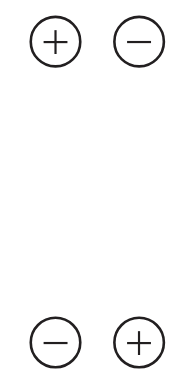
\includegraphics[width=0.3\textwidth]{uni1}
        \caption[]{\label{uni1}}
    \end{subfigure}
    \hfill
    \begin{subfigure}[b]{0.4\textwidth}
        \centering
        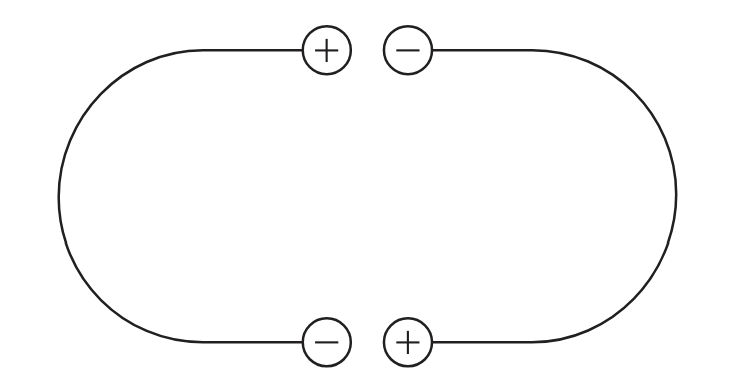
\includegraphics[width=\textwidth]{uni2}	
        \caption[]{\label{uni2}}
    \end{subfigure}
    
    \begin{subfigure}[b]{0.4\textwidth}
        \centering
        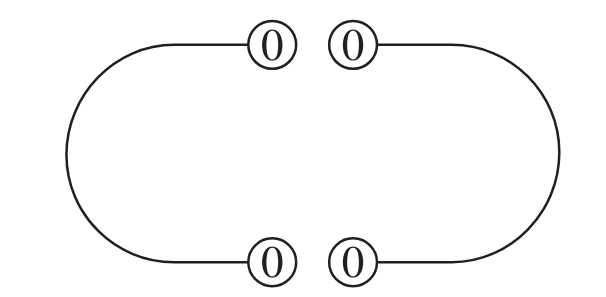
\includegraphics[width=\textwidth]{uni3}	
        \caption[]{\label{uni3}}
    \end{subfigure}
    
    \caption[]{\label{uni}}
\end{figure}

\section{The Method of Images}

Suppose a point charge \(q\) is held a distance \(d\) above an infinite grounded\footnote{Note that if the plate is instead held at potential \(V_0 \), or is isolated with net charge \(Q\) (which is equivalent to being held at potential \(V_0 \) but \(V_0 \) is now determined by the net charge \(Q\) of the conductor), then the solution is \href{https:////physics.stackexchange.com//questions//314982//method-of-image-charges-for-a-point-charge-and-a-non-grounded-conducting-plane}{highly non-trivial}.} conducting plane and we wish to find the potential in the region above the plane. From a mathematical standpoint, this is equivalent to solving the Poisson's equation in the region \(z > 0\), with \(\rho \) corresponds to a single point charge  \(q\) located at \((0,0,d )\), subject to the boundary conditions: 

\begin{enumerate}
    \item \(V = 0\) when \(z = 0\), and \item \(V \rightarrow 0\) for \(x^2 + y^2 + z^2 \gg d^2\).	
\end{enumerate}

By some clever insights, we see that for the potential created by a pair of opposite charge with \(q\) located at \((0,0,d)\) and \(-q\) located at \((0,0,-d)\) satisfy \(\rho \) in the region \(z > 0\).\footnote{We cannot place iamge charges in the volume \(V\) where we are calculating the potential, since for the first uniqueness theorem to stand, the charge density throughout the region has to be fixed as the given \(\rho \). Also the images charges must add up to the correct total in each region. (why?)} 

The essential idea is that there the potential created by the induced charge \((z>0)\) inside the region of interest \((z>0)\) can be replaced by the potential created by the image charge \((z<0)\) inside the region of interest \((z>0)\). Outside the region of interest, the two potentials created by the induced charge and the image charge are entirely different.  

Since the electric field is just \(\vb{E} = -\grad{V} \), it is also uniquely determined and the force that the real charge experience can be easily calculated as \( \vb{F} = -q^2\vu{z}/ 4\pi \epsilon_0 (2d)^2\).

The potential energy of the system can be found by integrating the force from infinity to \(d\) which yields 

\begin{equation}
    U = \int_{\infty}^{d}  \frac{q^2}{4\pi \epsilon _{0} (2z)^2} dz = -\frac{q^2}{16\pi \epsilon _{0} d} ,
\end{equation}

which is only half of the energy of a pair of real charge \(q \text{ and }  -q\) separated by a distance \(2d\). 

This is because there is no electric field in the region \(z < 0\), or equivalently, the image charge can be moved for free, since there isn't any electric field to oppose. 

So in general the energy becomes \(U = q_{\text{real} } V \) and we only need to take into account the energy of the real charges. 



\example{Image Charges of a Conducting Spherical Shell.}
{A point charge \(q\) is situated a distance \(a\) from the center of a conducting shell\footnote{A conducting sphere works just as fine here as well. This is because for \(a > R\), the real charge density is zero inside the shell, so the internal field can be found by solving the Laplace's equation with \(\rho = 0\) and subject to the boundary condition of constant potential at the shell. By invoking the first uniqueness theorem, we see that the internal field equals to zero which resembles the case of a conductor is the only answer.} of radius \(R < a\).\footnote{The same can be done for \(R > a\) but we omit here for simplicity.} Find the potential outside the spherical shell if it is  
\newline 
\begin{enumerate}[itemsep=10pt] 
    \item grounded,\footnote{Grounded means \(V = 0 \) relative to infinity, since it is connected to the Earth by a wire, and Earth has infinite capacitance, if we consider the Earth and the sphere as one conductor, we get \(V = 0\) from \(Q = CV\).} or
    \item held at potential \(V_0\), or
    \item isolated with net charge \(Q\).
\end{enumerate}~}
{\begin{enumerate}
    \item The problem is equivalent to solving the Laplace's equation for the region outside the sphere, subject to the boundary conditions: 
    
    \begin{enumerate}[itemsep=10pt] 
        \item \(V = 0\) on the surface of the sphere, and
        \item \(V \rightarrow 0\) for  \(x^2 + y^2 + z^2 \gg R\) .		
    \end{enumerate} 
    
    It so happens that the potential created by a point charge \(q' = -Rq /a\) located at \(R^2 /a \) from the center of the sphere (which always stay inside the sphere since \(R < a\)) together with the real charge satisfies both the boundary conditions and the charge density requirement. 
    
    Thus, by the first uniqueness theorem, the potential created by the two charges is our final and only answer.\newline 
    
    \item Now the boundary conditions are modified to be:
    
    \begin{enumerate}
        \item \(V = V_0\) on the surface of the sphere, and
        \item \(V \rightarrow 0\) for \(x^2 + y^2 + z^2 \gg R\).	 
    \end{enumerate}
    
    Then since from the first part we already know that the potential created by \(q \text{ and } q'\) is zero over the surface of the shell, we only need to add another image charge \(q''\) at the center of the shell (or over the surface of the shell) such that 
    
    \begin{equation}
        V_0 = \frac{1}{4\pi\epsilon_0} \frac{q''}{R}.
    \end{equation}
    
    We see that the potential created by \(q, q' \text{ and } q''\) satisfy both the charge density requirement as well as the boundary conditions. Therefore, we claim this as our answer. \newline
    
    \item In this part, the boundary conditions are identical to those in the previous part, except for the fact that \(V_0\) is not known but is determined by the total net charge \(Q\). Therefore we still have the same image charges configuration as the previous part but we need to find \(q''\), which depends on \(V_0 \), which depends on \(Q\).  
    
    To find \(q''\) we see that use the fact that the electric field outside the sphere created by the real net charge \(Q\), \textit{i.e.,} \(\vb{E} _{\text{real} } \) is identical as the electric field outside the sphere created by the image charges \(q_{\text{images} } \), \textit{i.e.,} \(\vb{E} _{\text{images} } \). So we have
    
    \begin{equation}
        \oint _{S} \vb{E}_{\text{real}}  \cdot d\vb{S} = \frac{Q}{\epsilon_0} = \oint _{S} \vb{E} _{\text{image}} \cdot d\vb{S} = \frac{q_{\text{images}}}{\epsilon_0} .
    \end{equation}
    
    Therefore we conclude that the total image charges is equal to the net charge, \textit{i.e.,} 
    
    \begin{equation}
        Q = q_{\text{images} } = q' + q''.
    \end{equation}
    
    And the rest is identical to the previous part.

    Note that we cannot simply substitute \(Q = 0\) in the above equation to find \(q''\) in the previous part, since \(Q \) denotes the net real charge, which is not equals to zero when the conductor is held at potential \(V_0 \). 

    Instead, using the above equation we can find the real induced charge of the spherical shell, wich is 

    \begin{equation}
        q_{\text{induced} } = q'+q'' = -\frac{R}{a} q + 4\pi \epsilon_0 RV_0 .   
    \end{equation}
\end{enumerate}~} 

\section{Separation of Variables}

The method of separations of variables used for tackling the Laplace's equation is best illustrated with examples.

\subsection{Cartesian Coordinates}

In the Cartesian Coordinates, the Laplace's equation reads
    
\begin{equation}
    \frac{\partial V}{\partial x}  + \frac{\partial V}{\partial y}  + \frac{\partial V}{\partial z}  = 0. 
\end{equation}
            
We seek a solution in the form of 
    
\begin{equation}
    V(x,y) = X(x)Y(y)Z(z).
\end{equation}
    
Of course, the solution need not to be in this form. However, if we do find a solution, by any means, that satisfy the Laplace's equation and its boundary conditions, then by the first uniqueness theorem, we know that it must be the only answer. 
    
Substituting our proposed solution and separating the variables,
    
\begin{equation}
    \begin{aligned}
        YZ \frac{d^2X}{dx^2} + XZ \frac{d^2Y}{dy^2} + XY \frac{d^2Z}{dz^2} &= 0 \\
        \frac{1}{X} \frac{d^2X}{dx^2} + \frac{1}{Y} \frac{d^2Y}{dy^2} + \frac{1}{Z} \frac{d^2Z}{dz^2} &= 0. 
    \end{aligned}
\end{equation}
    
Since we have an equation in the form of \(f(x) + g(y) + h(z) = 0\), the only way the this could possibly be true is that both  \(f,g \text{ and }  z\) must be constant or else I could say vary \(x\) while keeping \(y \text { and } z\) constant and the equality wouldn't hold. Thus, we have
    
\begin{equation}
    \frac{1}{X} \frac{d^2X}{dx^2} = C_1, \quad \frac{1}{Y} \frac{d^2Y}{dy^2} = C_2 ~ \text{ and } ~ \frac{1}{Z} \frac{d^2Z}{dz^2} = C_3, \quad C_1 + C_2 + C_3 = 0.
\end{equation}

\example{Separation of Variables in Cartesian Coordinates.}
{Find the potential \(V(x,y)\) bounded by the metal sheets fixed at potential \(V_0 (y)\) and infinity as shown in \cref{lap1}.}
{By symmetry, it is obvious that \(V\) is independent of \(z\), and the boundary conditions are
            
\begin{enumerate}[itemsep=10pt] 
    \item \(V = 0\) when \(y = 0 \text { and }  y = a\),
    \item \(V = V_0(y)\) when \(x = 0\), and
    \item \(V \rightarrow  0\) as \(x \rightarrow  \infty\).
\end{enumerate}

With the results derived, we have

\begin{equation}
    \frac{d^2X}{dx^2} = k^2X ~~~ \text{ and } ~~~ \frac{d^2Y}{dy^2} = -k^2Y
\end{equation}

where we rewrite the constant \(C_1 \text{ as } k^2\) since \(C_1\) should be positive and  \(C_2\) should be negative, such that \(V(x)\) will admit an exponential decaying function where \(V(x) \rightarrow 0\) as \(x \rightarrow \infty\) and \(V(y)\) will admit a sinusoidal function so that \(V(y)\) will vanish at \(y = 0\) and \(y = a\).            

which gives the solutions

\begin{equation}
    V(x,y) = (A e^{kx} + B e^{-kx} )(C\sin ky+D\cos ky) .
\end{equation}

Applying the boundary conditions 1 and 3 will left us with 

\begin{equation}
    V(x,y) = C e^{-kx} \sin ky, ~~~ \text{ where } k = \frac{n\pi }{a}. 
\end{equation}

Since the Laplace's equation is linear, the general solution is the linear combination of all solutions each with different \(n\), so we have 

\begin{equation}
    V(x,y) = \sum_{n=1}^{\infty} C_{n} \sin \frac{n\pi y}{a} e^{-\frac{n\pi x}{a}} .
\end{equation}

To satisfy the second boundary condition

\begin{equation}
    V(0,y) = \sum_{n=1}^{\infty} C_{n} \sin \frac{n\pi y}{a} = V_0(y) ,
\end{equation}

we have to rely on the Fourier's trick, where we multiply both sides by \(\sin \frac{m\pi y}{a} \) and integrate from \(0 \text { to } a\)

\begin{equation}
    \sum_{n=1}^{\infty} C_{n} \int_{0}^{a} \sin \frac{n\pi y}{a} \sin \frac{m\pi y}{a} dy = \int_{0}^{a} V_0(y) \sin \frac{m\pi y}{a} dy.			 
\end{equation}

Since 

\begin{equation}
    \int_{0}^{a} \sin \frac{n\pi y}{a} \sin \frac{m\pi y}{a} dy = \begin{cases}
        0 & \text{if } n \neq m, \\[10pt]
        a/2 & \text{if } n = m.
        \end{cases}
\end{equation}

Thus 

\begin{equation}
    C_{n}  = \frac{2}{a} \int_{0}^{a} V_0(y) \sin \frac{n\pi y}{a} dy.  
\end{equation}

If \(V_0(y) = V_0\), then 

\begin{equation}
    \begin{aligned}
        C_{n} &= \frac{2v_0}{a} \int_{0}^{a} \sin \frac{n\pi y}{a} dy = \frac{2V_0}{n\pi } (1 - \cos n\pi )  \\ 
        &= \begin{cases}
            ~ 0 &\text { if } n  \text{ is even}, \\
            \frac{4V_0}{n\pi } &\text { if } n \text{ is odd} .
        \end{cases} 
    \end{aligned}
\end{equation}

Thus

\begin{equation}
    V(x,y) = \frac{4V_0}{\pi } \sum_{\text{odd n}}^{} \frac{1}{n} \sin \frac{n\pi y}{a}  e^{\frac{-n\pi x}{a}}. 
\end{equation}

Incidentally, the result can be further simplified by writing \( \sin (in\pi y /a) \text{ as } \mathfrak{Re} ((-i)e^{n\pi y/a } )  \), then \(V(x,y) = 4V_0 I /a\), where

\begin{equation}
    I = \mathfrak{Re} \left(-i\sum_{\text{odd n}}^{} \frac{1}{n} \left(e^{-\frac{\pi (x-iy)}{a} }\right)^{n}\right) 
\end{equation}

Letting \( \mathcal{Z} = e^{-\pi (x-iy)/a }  \), we have

\begin{equation}
    \begin{aligned}
        \sum_{\text{odd n}}^{} \frac{\mathcal{Z} ^{n} }{n} &= \sum_{j=0}^{\infty} \frac{\mathcal{Z} ^{(2j+1)} }{2j+1} = \int_{0}^{\mathcal{Z} } \left(\sum_{j=0}^{\infty} u^{2j} \right)du = \int_{0}^{\mathcal{Z} } \frac{du}{1-u^2} \\
        &= \frac{1}{2} \ln (\frac{1+\mathcal{Z} }{1-\mathcal{Z} } ) = \frac{1}{2}  \ln (R e^{i\theta } ) = \frac{1}{2} (\ln R + i\theta )
    \end{aligned}
\end{equation}

where we have defined \(R e^{i\theta } \text{ as } (1+\mathcal{Z}) / (1-\mathcal{Z}) \). So \( I =  \mathfrak{Re}  ((-i) (\ln R + i\theta ) /2) = \theta /2 \). Since 
\begin{equation}
    \begin{aligned}
        &\frac{1+\mathcal{Z}}{1-\mathcal{Z}}=\frac{1+e^{-\pi(x-i y) / a}}{1-e^{-\pi(x-i y) / a}}=\frac{\left(1+e^{-\pi(x-i y) / a}\right)\left(1-e^{-\pi(x+i y) / a}\right)}{\left(1-e^{-\pi(x-i y) / a}\right)\left(1-e^{-\pi(x+i y) / a}\right)} \\
        & =\frac{1+e^{-\pi x / a}\left(e^{i \pi y / a}-e^{-i \pi y / a}\right)-e^{-2 \pi x / a}}{\left(1-e^{-\pi(x-i y) / a}\right)\left(1-e^{-\pi(x+i y) / a}\right)}=\frac{1+2 i e^{-\pi x / a} \sin (\pi y / a)-e^{-2 \pi x / a}}{\left(1-e^{-\pi(x-i y) / a}\right)\left(1-e^{-\pi(x+i y) / a}\right)}
    \end{aligned}
\end{equation}

for which the denominator is real, so

\begin{equation}
    \tan \theta=\frac{2 e^{-\pi x / a} \sin (\pi y / a)}{1-e^{-2 \pi x / a}}=\frac{2 \sin (\pi y / a)}{e^{\pi x / a}-e^{-\pi x / a}}=\frac{\sin (\pi y / a)}{\sinh (\pi x / a)}. 
\end{equation}


Therefore 
\begin{equation}
    I=\frac{1}{2} \tan ^{-1}\left(\frac{\sin (\pi y / a)}{\sinh (\pi x / a)}\right) \implies  V(x, y)=\frac{2 V_0}{\pi} \tan ^{-1}\left(\frac{\sin (\pi y / a)}{\sinh (\pi x / a)}\right) .
\end{equation}}

\onefig{lap1}{scale=0.3} 

\subsection{Spherical Coordinates}

Asuuming that the potential \(V\) is independent of \(\phi \), the Laplace's equation reads 

\begin{equation}
    \pdv{r} (r^2 \pdv{V}{r} ) + \frac{1}{\sin \theta } \pdv{\theta } (\sin \theta \pdv{V}{\theta } ) = 0.
\end{equation}

Substituting \(V(r,\theta ) = R(r)\Theta (\theta )\) and separating the variables, we have 

\begin{equation}
    \frac{1}{R} \frac{d}{dr} (r^2 \frac{dR}{dr} ) = l(l+1) ~~~ \text{ and } ~~~ \frac{1}{\Theta \sin \theta } \frac{d}{d\theta} (\sin \theta \frac{d\Theta}{d\theta} ) = -l(l+1)	
\end{equation}

where we have written the separation constant as \(l(l+1)\) where \(l\) is an positive integer, or else the solution would not be physical on the \(z\) axis as the series solution to the angular differential equation would not converge for \(\theta = 0 \text { or }  \pi \) explained \href{https://jfoadi.me.uk/documents/lecture_mathphys2_08.pdf}{here}.

For the radial ordinary differential equation, the general solution has the form

\begin{equation}
    R(r) = Ar^{l} + \frac{B}{r^{l+1} } .
\end{equation}

While for the angular ordinary differential equation, the general solutions are Legendre polynomials in the variable \(\cos \theta \), where is given by the Rodrigues formula

\begin{equation}
    P_{l}(x) = \frac{1}{2^{l} l!} \left(\frac{d}{dx} \right)^{l} (x^2 - 1)^{l} . 
\end{equation}

The first few Legendre Polynomials are \(P_0(x) = 1, ~P_1(x) = x \text{ and } P_2(x) = \frac{3x^2 - 1}{2} \). Also, with the factor \(\frac{1}{2^{l} l!} \) introduced, we have \(P_{l} (1) = 1\).  

However since the angular differential equation is second order, it should possess two independent solutions for every value of \(l\). It turns out that the other solution blow up at the \(z\) axis anyways and is eliminated by initial or boundary conditions such that the coefficient introduced due to the linearity of the differential equation becomes zero.

From the linearity of the Laplace's equation, the general solution is

\begin{equation}
    V(r,\theta ) = \sum_{l=0}^{\infty} (A_{l} r^{l} + \frac{B_{l} }{r^{l+1} } )P_{l} (\cos \theta). \label{sphlap1} 
\end{equation}

\example{Separation of Variables in Spherical Coordinates (1).}
{Find the potential in all space if \(V_0(\theta )\) is specified on a spherical shell of radius \(R\).}
{For the region inside the shell, we immediately see that \(B_{l} = 0\) otherwise the potential would blow up at the origin. Also, we require that 

\begin{equation}
    V(R,\theta ) = \sum_{l=0}^{\infty} A_{l} R^{l} P_{l} (\cos \theta ) = V_{0} (\theta )
\end{equation}

We again use the Fourier's trick, but this time we multiply by \(P_{l'} (\cos \theta )\) and use the fact that 

\begin{equation}
    \begin{aligned}
        \int_{-1}^{1} P_{l} (x) P_{l'} (x) dx &= \int_{0}^{\pi } P_{l} (\cos \theta ) P_{l'} (\cos \theta ) \sin \theta d\theta \\ &= \begin{cases}
            ~~0 & \text{if } l' \neq l \\[10pt]
            \frac{2}{(2l+1)}  & \text{if } l' = l.
            \end{cases}
    \end{aligned}
\end{equation}

Thus by similar means as the previous example, we get

\begin{equation}
    A_{l} = \frac{2l+1}{2R^{l} } \int_{0}^{\pi } V_{0} (\theta ) P_{l} (\cos \theta ) \sin \theta d\theta.
\end{equation}

The integrals can be difficult to evaluate and in practice it is often easier to solve for \(A_{l} \) by observation. For example, if \(V_0(\theta ) = k\sin ^2\left(\theta /2\right)\), then we can rewrite this as

\begin{equation}
    V_0(\theta ) = \frac{k}{2} (1-\cos \theta ) = \frac{k}{2} (P_0(\cos \theta ) - P_1(\cos \theta )).
\end{equation}

So we immediately read off from \cref{sphlap1} that \( A_0 = k /2 \text{ and }  A_1 = -k /2R \) and

\begin{equation}
    V(r,\theta )  = \frac{k}{2} (1 - \frac{r}{R} \cos \theta ).
\end{equation}	

And if \(V_0(\theta) = k\cos (3 \theta)\), then we can rewrite this as

\begin{equation}
    V_0(\theta) = k(4\cos ^3 \theta - 3\cos \theta) = \frac{k}{5} (8P_3 (\cos \theta) - 3P_1(\cos \theta)).
\end{equation}

So we can find that \(A_1 = -3k /5R \text{ and } A_3 = 8k /5R^3  \) and 

\begin{equation}
    V(r,\theta) = kr \cos \theta /5R  \left(4\left(r /R\right)^2(5\cos ^2 \theta-3)-3\right). 
\end{equation}} 


\example{Separation of Variables in Spherical Coordinates (2).}
{Find the potential in the region outside of an uncharged metal sphere of radius \(R\) placed in an otherwise unifrom electric field \(\vb{E} = E_0 \vu{z} \).}
{Since \(V\) does not goes to zero at infinity, we redefine the potential to be zero at the surface of the sphere (since it is an equipotential surface). Then the boundary conditions becomes
    
\begin{enumerate}[itemsep=10pt] 
    \item \(V = 0 \text { at } r = R\),
    \item \(V \rightarrow -E_0z = -E_0r\cos \theta \text { for } r \gg R\). 
\end{enumerate}

Applying the first boundary condition gives

\begin{equation}
    V(r,\theta ) = \sum_{l=0}^{\infty} A_{l} \left(r^{l}  - \frac{R^{2l+1} }{r^{l+1} } \right) P_{l} (\cos \theta ). 			
\end{equation}

And the second boundary condition requires that 

\begin{equation}
    \sum_{l=0}^{\infty} A_{l} r^{l} P_{l} (\cos \theta ) = -E_0 r\cos \theta .  
\end{equation}

Thus, we read off \(A_{l} = 0\) except for \(A_1 = -E_0 \) and the potential is 

\begin{equation}
    V(r,\theta ) = -E_0 \left(r-\frac{R^3}{r^2} \right) \cos \theta 
\end{equation}

where the first term is due to the external field and the second term is contributed by the induced charge.

The induced charge density can be calculated by 

\begin{equation}
    \sigma (\theta ) = -\epsilon_0 \eval{\pdv{V}{r} }_{r=R}^{} = 3 \epsilon_0	E_0 \cos \theta  
\end{equation}} 

\example{Separation of Variables in Spherical Coordinates (3).}
{A specified charge density \(\sigma_0(\theta)\) is glued over the surface of a spherical shell of radius \(R\). Find the resulting potential inside and outside the sphere without using \cref{potential}.}
{We start with 

\begin{equation}
     V(r, \theta) =
    \begin{cases}
    \sum_{l=0}^{\infty} A_{l}r^{l}P_{l}(\cos \theta )    & \text{for } r \leq R, \\[10pt]
    \sum_{l=0}^{\infty} \frac{B_{l} }{r^{l+1} } P_{l}(\cos \theta ) & \text{for } r \geq R.
    \end{cases}  
\end{equation}

The boundary conditions are that the two potentials must be the same at \(r = R\) and the difference in nomral derivatives is due to the presence of the surface charge. So

\begin{equation}
    \sum_{l=0}^{\infty} A_{l}R^{l}P_{l}(\cos \theta ) = \sum_{l=0}^{\infty} \frac{B_{l} }{R^{l+1} } P_{l}(\cos \theta ) ~\text { and }~ \eval{\left( \frac{\partial V_{\text{out} } }{\partial r} - \frac{\partial V_{\text{in} } }{\partial r}   \right)}_{r=R}^{} = -\frac{\sigma _{0}(\theta ) }{\epsilon _{0} }.         
\end{equation}

They combined to give 

\begin{equation}
    A_{l} = \frac{1}{2\epsilon _{0}R^{l-1}  } \int_{0}^{\pi } \sigma _{0}(\theta ) P_{l}(\cos \theta ) \sin \theta d \theta ~\text { and }~ B_{l} = A_{l}R^{2l+1}.       
\end{equation}

For instance, if \(\sigma _{0} = k\cos \theta  = kP_1 (\cos \theta )\), then \(A_1  = k /3 \epsilon _{0} \) which impiles 

\begin{equation}
      V(r, \theta) =
    \begin{cases}
    kr \cos \theta / 3 \epsilon _{0}, & \text{for } r \leq R \\[10pt]
    kR^3 \cos \theta / 3\epsilon _{0}r^2  & \text{for } r \geq R.
    \end{cases}  
\end{equation}

In particular, we found from the previous example that the induced charge of a metal sphere under an otherwise uniform electric field \(\vb{E} = E_0 \vu{z} \) is \(\sigma _{0}(\theta ) = 3 \epsilon _{0}E_0   \). Subsituting \(k = 3 \epsilon _{0}E_0  \), we see that the potential inside is \(V(r,\theta ) = E_0 r \cos \theta = E_0 z\) and the field is \(- E_0 \vu{z} \) which cancels out the external field \(E_0 \vu{z} \), as it should.      
} 

The success of the method of separation of variables hinges on two extraordinary properties of the separable solutions, namely the completeness and orthogonality. In linear algebra terms, the set of functions is an orthonormal basis of the set of all real functions.

A set of functions \(f_{n} (y)\) is said to be complete if any other function \(f(y)\) can be expressed as a linear combination of them, \textit{i.e.,} 

\begin{equation}
    f(y) = \sum_{n=1}^{\infty} C_{n} f_{n} (y). 
\end{equation}

For example, the functions \(\sin \frac{n\pi y}{a}\), where \(n\) are positive integers are complete over the interval \(0~\le~y\le~a\) as guaranteed by Dirichlet's theorem. Also, any \(n^{\text{th }} \)  order polynomials can be expressed as the linear combination of the first \(n+1\) Legendre's polynomials, as the set of functions \(P_{l} (x)\) is complete for polynomials.

Orthogonality, on the other hand, means that the integral of the product of any two distinct members of the set is zero, \textit{i.e.,}  
\begin{equation}
    \int_{0}^{a} f_{n} (y) f_{n'} (y) dy = 0 \text { for }  n' \neq n. 
\end{equation}

It is this property that allows us to perform the Fourier's trick.


\chapter{Electric Field in Matter}

\section{Multipole Expansion and Dipole moment}

Referring to \cref{multipoleexpansion}, suppose we are trying to find the potential (or equivalently, electric field) of a point \(P\) in space far away from the source charges. We then have 

\onefig{multipoleexpansion}{scale=0.3} 

\begin{equation} \label{1drj} 
    \begin{aligned} 
    \frac{1}{\rcurs } &= \frac{1}{ r \sqrt{1 - 2\cos \alpha \left( \frac{r'}{r}  \right) + \left( \frac{r'}{r}  \right)^2}} \equiv \frac{1}{r} (1 + \epsilon )^{-\frac{1}{2} } = \frac{1}{r} \left( 1 - \frac{1}{2}\epsilon  + \frac{3}{8} \epsilon ^2 + \frac{5}{16} \epsilon ^3 + \cdots  \right) \\
    &=\frac{1}{r} \left( 1 + \cos \alpha \left( \frac{r'}{r}  \right) + \left( \frac{3\cos ^2\alpha -1}{2} \right) \left( \frac{r'}{r}  \right)^2 -\frac{5}{16} \left( \frac{5\cos ^3 \alpha - 3\cos \alpha }{2} \right) \left( \frac{r'}{r} \right)^3 + \cdots \right) \\
    &= \frac{1}{r} \sum_{n=0}^{\infty} \left( \frac{r'}{r}  \right)^{n} P_{n}(\cos \alpha ),  
    \end{aligned} 
\end{equation}

where \(\alpha \) is the angle between \(\vb{r} \text { and } \vb{r} '\) and \(P_{n}\) is the \(n^{\text{th }} \) Legendre polynomials.    

Substituting back into \cref{comb}, we have 

\begin{equation}
    \begin{aligned} 
    V(\vb{r} ) &= \frac{1}{4\pi \epsilon _0} \sum_{n=0}^{\infty} \frac{1}{r^{n+1} } \int r'^{n} P_{n}(\cos \alpha )\rho (\vb{r} ')d\tau ' \\
    &= \frac{1}{4\pi \epsilon_0} \left( \frac{1}{r} \int \rho (\vb{r} ')d\tau ' + \frac{1}{r^2}\int r'\cos \alpha \rho (\vb{r} ')d\tau ' + \cdots  \right) 
    \end{aligned} 
\end{equation}

The first term is the monopole contribution, telling that if we are sufficiently far away from the source, then we can treat the charge distribution as a point charge at the origin, which vanishes if the total charge is zero.

The second term is the dipole contribution, which can be written as 

\begin{equation}
    V_{\text{dip} } (\vb{r} ) = \frac{1}{4\pi \epsilon_0r^2} \left( \vu{r}  \cdot \int \vb{r} ' \rho (\vb{r} ')d\tau '  \right) = \frac{\vb{p} \cdot \vu{r} }{4\pi \epsilon _0 r^2 }.    \label{dippotential} 
\end{equation}

Analagous to a point charge at the origin where its potential is exactly given by the first term of the multipole expansion, a perfect dipole whose potential is exactly given by the second term of the multipole expansion is when 

\begin{equation}
    \vb{p} = \lim_{\vb{d}  \to 0, q \to \infty} q\vb{d}  
\end{equation}

and is located at the origin. 

The terms in the multipole expansion generally depends on the choice of origin. however, if the total charge is zero, then the dipole term is independent of the choice of origin. This is also the reason why the dipole moment of two opposite charge with the same magnitude \(q\) is simply \(\vb{p} = q\vb{d} \), where \(\vb{d} \) is the displacement vector from the negative charge to the positive charge. 

Placing the dipole at the origin, orienting \(\vb{p} \) to point in the \(z\) direction and taking the negative gradient of the potential contributed by the dipole term, we get the electric field created by a dipole as

\begin{equation}
    \vb{E} _{\text{dip} } (r, \theta ) = \frac{p}{4\pi \epsilon _0 r^3 }(2\cos \theta \vu{r} + \sin \theta \vu{\boldsymbol{\theta } }). 
\end{equation}

In fact, a quick way to generate the multipole potential is to simply take the gradient of the lower order potential, for example, to generate diopole potential from the monopole potential, we can imagine a negative charge \(-q\) located at \(\vb{r} '_{-}  \) and a positive charge \(+q\) located at \(\vb{r}' _{+}  \). Then the dipole potential is the combination of the monopole potential

\begin{equation}
    V_{\text{dip} } (\vb{r} ) = V_{\text{mono,+q} } + V_{\text{mono,-q} } = V_{\text{mono} }\left( \vb{r} - \frac{\vb{d} }{2}  \right) - V_{\text{mono} } \left( \vb{r} + \frac{\vb{d} }{2}  \right) = - \grad{V} \cdot \vb{d} = \frac{k \vb{p} \cdot \vu{r} }{r^2}. 
\end{equation}

Ultimately, this method boils down to the fact that if \(V (\vb{r} )\) is a solution to the Laplace's equation, \textit{i.e.,} \(\laplacian V = 0\), then its gradient \(\grad{V(\vb{r} )} \) also is, since \(\laplacian (\grad{V(\vb{r} )} ) = \grad{\laplacian V(\vb{r} )} = 0 \), due to the linearity of the differential operators. Note that \(\rho (\vb{r} ) = 0\) everywhere, including the origin where the charges cancel out.








\section{Polarization}

A material can be classified into either a conductor, where there are unlimited supply of free charges that can move around, or an insulator (or dielectric), where there are no free charges that can move around the material. 

Just as a conductor will response to an external electric field \(\vb{E} _{\text{ext} } \)  by moving the free charges around which creates an opposing electric field that cancels out with the external one, such that the electric field inside a conductor is zero, a dielectric material would also response to an electric field in a similar way, cancelling the external electric field partially. In fact, a conductor is merely an extreme case of a very bad insulator (\(\chi _{e} \to \infty\) ).

This is because the electric field will cause a lot of little electric dipoles to appear, for which the effect is measured by the polarization \(\vb{P} \) which is the dipole moment per unit volume. The two mechanisms causing the polarization are not important but are stated below.

The relation between \(\vb{P} \text { and } \vb{E} \) of a material is charizterized by its electric susceptibility 

\begin{equation}
    \vb{P} = \epsilon _{0} \chi _{e}\vb{E}_{\text{tot} }.
\end{equation}

An important point to note here is that \(\vb{E} _{\text{tot} } \) comprise of both the electric field which already exists before the polarization, as well as the electric field created by the induced bound charges due to polarization. 

\subsection{Ionization of Non-Polar Atoms}

As the force experienced by the positive nucleus and the negative electron cloud is in opposite direction, they will drift towards opposite direction until the attraction force between the nucleus and the electron cloud balance the the electric force exerted by the external electric field. The induced dipole moment of the atom \(\vb{p} \) is given in terms of the atomic polarizability \(\alpha \) as \(\vb{p} = \alpha \vb{E}_{ext}  \).

\example{Atomic Polarizability.}
{Calculate the atomic polarizability for an atom with radius \(\vb{a} \) and nucleus charge \(+q\).}
{Let \(d\) be the distance between the nucleus and the center of the electron cloud when the atomic reaches an equilibrium state. Balancing the forces on the nucleus (or the electron cloud), we have

\begin{equation}
    qE_{\text{ext} }  = q \frac{1}{4\pi \epsilon_0} \frac{qd}{a^3 }.
\end{equation}

The atomic polarizability is therefore 

\begin{equation}
    \alpha = \frac{p}{E_{ext} } =  \frac{qd}{E_{ext} } = 4\pi \epsilon _0 a^3 = 3\epsilon _0 V. 
\end{equation}
} 

\subsection{Alignment of Polar Molecules} \label{alignpolar} 

The force and the torque about its center expereinced by a molecule (which we model as an electric dipole) is 

\begin{equation}
    \vb{F} = q(\Delta \vb{E} ) = q (\vb{d} \cdot \grad{} )\vb{E}  = (\vb{p}  \cdot \boldsymbol{\nabla }) \vb{E} ~\text { and }~ \vb{N} = \vb{p} \cross \vb{E}
\end{equation}

and the energy of a dipole is 

\begin{equation}
    U = q(V(\vb{r} + \vb{d} ) - V(\vb{r} )) = q\Delta V(\vb{r} ) = q\grad{V(\vb{r} )}\cdot \vb{d} = - \vb{p} \cdot \vb{E}. 
\end{equation}

So the molecules will align themselves towards the direction of the elctric field in order to achieve minimum energy. 

Alternatively, this result can be proved by virtual work principle, by imagining that the 

\section{Electric Fields of Polarized Objects}

To calculate the electric field due to a polairized object, we notice that the electric potential from \cref{dippotential} reads

\begin{equation}
    \begin{aligned} 
    V(\vb{r} ) &= \frac{1}{4\pi \epsilon_0} \int_{V}^{} \frac{\vb{P} (\vb{r} ')\cdot \hrcurs }{\rcurs ^2}d\tau ' = \frac{1}{4\pi \epsilon_0} \int_{V}^{} \vb{P} \cdot \boldsymbol{\nabla '}\left( \frac{1}{\rcurs }  \right) d\tau ' \\
    &= \frac{1}{4\pi \epsilon_0} \left( \int_{V}^{} \boldsymbol{\nabla '} \cdot \left( \frac{\vb{P} }{\rcurs }  \right) d\tau ' - \int_{V}^{} \frac{1}{\rcurs } (\boldsymbol{\nabla '} \cdot \vb{P}  ) d\tau ' \right) \\
    &= \frac{1}{4\pi \epsilon_0} \left( \oint_{S} \frac{1}{\rcurs }\vb{P} \cdot d\vb{S} '  - \int_{V}^{} \frac{1}{\rcurs } (\boldsymbol{\nabla '} \cdot \vb{P}  ) d\tau ' \right) \\
    &\equiv  \frac{1}{4\pi \epsilon_0} \left( \oint_{S} \frac{\sigma _{b}(\vb{r} ') }{\rcurs } dS' + \int_{V}^{} \frac{\rho _{b} (\vb{r} ')}{\rcurs } d\tau ' \right),
    \end{aligned} 
\end{equation}

where \(\sigma _{b} = \vb{P} \cdot \vu{n} \text { and } \rho _{b} = - \div{\vb{P} } \) are the surface and volume charge density result from the polarization respectively.

The introduction of surface and volume bound charges is not merely a bookeeping tool, but are in fact visualizable. 

For surface bound charge, we imagine a long string of dipoles, where the positive head of one cancels the negative tail of its neighbor, so what left is the plus hand and the minus tail.

Since \(p = qd = PAd\) is the diopole moment of one individual dipole, we have the surface charge density as \(\sigma _{b} = 1 /A = P\), where the dot product with the normal unit vector is introduced to take into account if the end surface is not perpendicular to the polarization, then the area would be larger by a factor of \(\cos \theta \), where \(\theta \) is the angle between the polarizatoin and the unit normal vector.

For volume bound charge, we imagine some volume with non-zero divergence of polarization. Then by conservation of charge we have the amount positive charges reside on the surface of the volume (which in this case are effectively surface charges) is equal to amount of the negative charge inside the volume, so

\begin{equation}
    \int_{V}^{} \rho _{b} d\tau = - \oint_{S} \vb{P} \cdot d\vb{S} = - \int_{V}^{} (\div{\vb{P} } )d\tau . 
\end{equation}

Therefore, we can first calculate these induced bound charge (which are charges result from polarization) then calulcate the electric field via normal means.

\example{Uniformly Polarized Sphere (1).}
{Find the electric field of an uniformly polarized sphere of radius \(R\) and polarization \(\vb{P} \).}
{The surface and volume charge density are

\begin{equation}
    \sigma _{b} = \vb{P} \cdot \vu{n} = P\cos \theta  ~\text { and }~ \rho _{b} = - \div{\vb{P} } = 0.  
\end{equation}

But the problem of finding the potential of a surface charge density \(\sigma _{0} (\theta ) = k\cos \theta  \) glued on a sphere has alrady been solved in an example in the previous chapter. The result therefore is

\begin{equation}
 V(r, \theta) =
    \begin{cases}
    Pr \cos \theta / 3\epsilon _{0}  & \text{for } r \leq R, \\[10pt]
    PR^3 \cos \theta /3\epsilon _{0}r^2  & \text{for } r \geq R.
    \end{cases}  
\end{equation}

The electric field inside the sphere is 

\begin{equation}
    \vb{E} = -\grad{V} = - \frac{\vb{P} }{3\epsilon _{0} }\vu{z} = - \frac{\vb{P} }{3 \epsilon _{0} } \text{ for } r \le R
\end{equation}

while the potential outside the sphere is 

\begin{equation}
    V = \frac{1}{4\pi \epsilon_0} \frac{\vb{p} \cdot \vu{r} }{r^2} \text{ for } r \ge R, 
\end{equation}

which is indentical to that of a perfect dipole at the origin with dipole moment \(\vb{p} = \frac{4}{3}\pi R^3 \vb{P}  \) which is the total dipole moment of the sphere. 
} 

\example{Uniformly Polarized Sphere (2).}
{Analyze the same uniformly polarized sphere in the previous example by considering two overlapping spheres of charges \(+q\text { and } -q\).}
{The total electric field inside the overlapping region is the sum of the electric field of the individual spheres, which can be shown to be equals to

\begin{equation}
    \vb{E} = -\frac{1}{4\pi \epsilon_0} \frac{q\vb{d} }{R^3 } = -\frac{\vb{P} }{3\epsilon _{0} } 
\end{equation}

For the region outside the spheres, it is as though all the cahrges on each sphere were concentrated at the respective centers. We have then a dipole with potential 

\begin{equation}
    V(\vb{r} ) = \frac{1}{4\pi \epsilon_0} \frac{\vb{p} \cdot \vu{r} }{r^2}. 
\end{equation}
} 

\section{Microscopic and Macroscopic Fields}

When we say the electric field inside a point in matter, we do not mean the acutual microscopic electric field at that point, as the microscopic fields are actually highly non-uniform. What we mean is always the average electric field over a small region which is large enough to smooth over the uninteresting microscopic fluctuations and yet small enough to not wash out any significant large-scale variations in the field. So we are actually finidng the average electric field \(\vb{E} (\vb{r} )\) within the material by averaging the true microscopic field over a small sphere about \(\vb{r} \).

For the charges outside the sphere, we have proved in an example in \cref{lapeq} that the average electric field over a sphere is the equal to the field they produce at the center, so we can safely use

\begin{equation}
    V_{\text{out} } = \frac{1}{4\pi \epsilon_0} \int_{\text{outside} }^{} \frac{\vb{P} (\vb{r} ') \cdot \hrcurs }{\rcurs ^2} d\tau '.   
\end{equation}

The term left out in this integral is 

\begin{equation}
    V_{\text{in} } = \frac{1}{4\pi \epsilon_0} \int_{\text{in} }^{} \frac{\vb{P} (\vb{r} ') \cdot \hrcurs }{\rcurs ^2} d\tau ' = \frac{\vb{P} }{4\pi \epsilon_0} \cdot \int_{\text{in} }^{} \frac{\hrcurs }{\rcurs ^2}d\tau ',    
\end{equation}

where we have assume that the sphere is small enough for \(\vb{P} \) to be uniform. This is in fact just the potential at the center of the sphere due to a uniformly polarized sphere, and according to the examples in the previous section, the field is equals to \(\vb{E} _{\text{in} } = -\vb{P} /3 \epsilon_0  \). 

We have left out \(V_{\text{in} } \), since we cannot simply take the field at the center created by the charge inside the sphere as the average field over the sphere, which is what we want.

To calculate the correct average electric field due to the charges inside the sphere, we have proved in the example that the average electric field over a sphere is 

\begin{equation}
    \vb{E} _{\text{in} } = - \frac{\vb{p} }{4\pi \epsilon_0 R^3 } = -\frac{\left( \frac{4}{3}\pi R^3   \right)\vb{P} }{4\pi \epsilon_0 R^3 } = -\frac{\vb{P} }{3\epsilon_0 }.    
\end{equation}

We see that the average electric field is in fact the same as the electric field at the center, this is ultimately due to the fact that the field inside a uniformly polarized sphere is uniform, so the field is \(\vb{E} = - \vb{P} /3\epsilon_0 \) anywhere anyways. Therefore, we simply have 

\begin{equation}
    V = \frac{1}{4\pi \epsilon_0} \int \frac{\vb{P} (\vb{r} ')\cdot \hrcurs }{\rcurs ^2} d\tau ',  
\end{equation}

without having to split the integral into two parts.




\section{Modified Gauss's Law} \label{mode} 

While Gauss's law (\cref{gauss}) works completely fine inside polarized matter, where the electric field \(\vb{E} (\vb{r} )\) at a point \(\vb{r} \) is still related to the charge density \(\rho (\vb{r} )\)  by \(\div{\vb{E}(\vb{r} )} = \rho(\vb{r} ) / \epsilon_0 \), it is kind of useless since we do not know what \(\rho (\vb{r} )\) is: it composed of \(\rho = \rho _{f} + \rho _{b}  \), where the free charges \(\rho _{f} \) are the charges we can control and not arised from polarization while the bound charges \(\rho _{b} \) are the charges due to polarization of the material under an external electric field. 

Separating the charges into free charges and bound charges, we have

\begin{equation}
    \epsilon_0 \div{\vb{E} } = \rho _{f} + \rho _{b} = \rho _{f} - \div{\vb{P} }  \implies  \div{(\epsilon_0 \vb{E} +P)} \equiv \div{(\epsilon_0 \vb{E} + \epsilon_0 \chi _{e}\vb{E}  )} \equiv \div{(\epsilon \vb{E}) } \equiv  \div{\vb{D} } = \rho _{f},
\end{equation}

where \(\chi _{e} \) is the electric permittivity of the material, which relates the polarization \(\vb{P} \) of the material under an external electric field \(\vb{E} \), and \(\vb{D} \) is the electric displacement.    

So the ordinary Gauss's law can be rewritten to the modified Gauss's law

\begin{equation}
    \div{\vb{D} } = \rho _{f}. 
\end{equation}

The electric displacemnet is a useful quantity as when we put free charge in place, the only thing we know would be \(\vb{D} \) from the modified Gauss's law (instead of \(\vb{E} \) since we do not know \(\vb{P} \)).

However, we shall not assume that the relation between \(\vb{D} \text { and } \rho _{f} \) is the same as \(\vb{E} \text { and } \rho \). Although the divergences are analogous, the curl of \(\vb{E} \) is always zero while the curl of \(\vb{D} \) is \(\curl{\vb{D} } = \curl{\vb{P} } = \epsilon _{0}  \curl{(\chi _{e} \vb{E})}  \), which is not necessarily zero.

But for the case of homogenous medium, where the electric susceptibiliy \(\chi _{e} \) does not vary with position, we can take \(\chi _{e} \) out of the curl and we can safely regard \(\rho _{f} \) as the source of \(\vb{D} \) just as how \(\rho \) serves as the source of \(\vb{E} \).        

For ionic crystal such as sodium chloride, where the polarization and thus electrical displacement is ill-defined as the direction of a dipole moment of two oppositely charged ions depends on how you pair them up. But it does not matter. At the end of the day everyone agrees that the charge density and the electric field is zero.  

\example{Separation of Variables in Spherical Coordinates (4).}
{A sphere of homogeneous linear dielectric material of relative permittivity \(\epsilon _{r} \) is placed in an otherwise uniform electric field \(\vb{E} _{0} \). Find the electric field inside the sphere.}
{Defining the zero potential at the center of the sphere, we need to solve the Laplace's equation subject to the boundary conditions

\begin{enumerate}[itemsep=10pt] 
    \item $V_{\text{in}} = V_{\text{out}}$ at $r = R$,
    \item \(\epsilon \partial V_{\text{in} } / \partial r = \epsilon _{0} \partial V_{\text{out} } /\partial r  \)  at $r = R$, and
    \item $V_{\text{out}} \to -E_0 z = -E_0 r \cos\theta$ for $r \gg R$.
\end{enumerate}

Inside the sphere, we have

\begin{equation}
    V_{\text{in} }(r, \theta ) = \sum_{l=0}^{\infty} A_{l} r^{l}P_{l}(\cos \theta ),
\end{equation}

where \(B_{l} = 0\) for all \(l\) to avoid singularities at the origin. 

Outside the sphere, we have

\begin{equation}
    V_{\text{out} }(r,\theta ) = -E_0 r\cos \theta + \sum_{l=0}^{\infty}\frac{B_{l} }{r^{l+1} }P_{l}(\cos \theta ),   
\end{equation}

where \(A_{l} = 0 \) for all \(l\) except \(A_1 = -E_0 \) to satisfy the third boundary condition.

Solving for \(A_{l} \text { and } B_{l}  \) with the first and second boundary conditions, we get 

\begin{equation}
    \begin{cases}
        A_l = B_l = 0 & \text{for } l \neq 1, \\[10pt]
        A_1 = - 3E_0 / (\epsilon _{r}+2 ), \\[10pt]
        B_1 = (\epsilon _{r}-1 )E_0 /(\epsilon _{r}+2 )R^3.
        \end{cases}   
\end{equation}

The potential and electric field inside the sphere are thus

\begin{equation}
    \begin{cases}
        V_\text{in}(r, \theta) = -3 E_0 z /(\epsilon _{r}+2 ), \\[10pt]
        \mathbf{E} = 3E_0 /(\epsilon _{r}+2 ).
        \end{cases}
\end{equation}

Note that \(\vb{E} = 0\) when \(\epsilon _{r} \to \infty\) as it should in the case of a conductor, and \(\vb{E} = \vb{E} _{0} \) when \(\epsilon _{r} = 1 \) as it should in the case of vaccum.    
} 

\example{Image Charge of an Infinite Dielectric Plane.}
{Suppose the entire region below the plane \(z=0\) is filled with uniform linear dielectric material of susceptibility \(\chi _{e} \). Calculate the force on a point charge \(q\) situated a distance \(d\) above the origin.}
{First of all, the volume bound charge is zero, since

\begin{equation}
    \rho _{b} = - \div{\vb{P} } = - \div{\left( \vb{D} - \epsilon _{0}\vb{E} \right)} = - \div{\left( \left(1- \frac{\epsilon _{0} }{\epsilon } \right) \vb{D} \right)} = - \left( 1- \frac{1}{\epsilon _{r} }  \right) \rho _{f} = 0.   \label{boundfree} 
\end{equation}

The surface bound charge, on the other hand, is

\begin{equation}
    \sigma _{b} = \vb{P} \cdot \vu{n} = \epsilon _{0} \chi _{e}E_{z},    
\end{equation}

where \(E_{z} \) is the \(z-\)component of the total electric field just inside the dielectric at \(z=0\). This field is due in part to \(q\) and in part to the bound charge itself, so 

\begin{equation}
    E_{z} = - \left( \frac{1}{4\pi \epsilon_0} \frac{qd}{(r^2+d^2)^{\frac{3}{2} } } + \frac{\sigma _{b} }{2\epsilon _{0} }  \right).
\end{equation}

Solving for \(\sigma _{b} \), 

\begin{equation}
    \sigma _{b} = - \frac{1}{2\pi }\left( \frac{\chi _{e} }{\chi _{e}+2 }  \right)\frac{qd}{(r^2+d^2)^{\frac{3}{2} } }.   
\end{equation}

The electric field can be calculated by direction integration from \cref{comb} having known \(\sigma _{b} \). Alternatively, we note that we can place an image charge at \((0,0,-d)\) with charge \( q_{b} = -\chi _{e}q/(\chi _{e}+2 )   \) we have the correct potential in the region \(z > 0\). For region \(z < 0\), we can place the same point charge at \((0,0,d)\).

Therefore the force is 

\begin{equation}
    \vb{F} = - \frac{1}{4\pi \epsilon_0} \left( \frac{\chi _{e} }{\chi _{e}+2 }  \right) \frac{q^2}{4d^2}\vu{z} . 
\end{equation}
} 

\section{Energy in Dielectric Systems}

The general formula for the electric energy \( U = (\epsilon _{0}/2 ) \int E^2d\tau  \) is generally not used in dielectric system. This is because this is the work done needed if we assemble the system by bringing in all the charges (free and bound), one by one, with tweezers to its proper final location. 

This energy, however, just not include the work done need stretch and rotate the atoms or molecules, which can be modelled as a spring's energy \(kx^2 /2 \),\footnote{For example, the restoring force of ionizing an atom is proportional to the relative displacement of the nucleus and the center of the electron cloud. So the energy is proportional to the displacemnet squared} which, although is electrical in nature, is not accounted in the macroscopic field \(\vb{E} \). 

The energy we are interested in, is the work done required to introduce all the free charges one by one to achieve the final configuation, while the energy due to bound charges are subtly accounted as the when we bring in an infinitesimal free charge, it also has to overcome the electric field created by the bound charge. Specifically, the infinitesimal work done required is 

\begin{equation}
    \begin{aligned} 
    \Delta W &= \int (\Delta \rho _{f} ) V d\tau = \int \left( \div{(\Delta \vb{D} )}  \right) Vd\tau = \int \div{\left( (\Delta \vb{D} ) V\right)} d\tau + \int \left( \Delta \vb{D}  \right) \cdot \vb{E} d\tau \\
    &= \oint_{S} \left( (\Delta \vb{D} )V \right) \cdot d\vb{S} + \int \left( \Delta \vb{D}  \right) \cdot \vb{E} d\tau = \int \epsilon (\Delta \vb{E} )\cdot \vb{E} d\tau = \frac{1}{2}\int \vb{D} \cdot \vb{E} d\tau . 
    \end{aligned} 
\end{equation}

where the potential is constant since we are bringing an infinitesimal charge into the system, so the potential should be the pre-exisiting potential.

So the total energy of a dielectric system is 

\begin{equation}
    U = \frac{1}{2} \int \vb{D} \cdot \vb{E} d\tau  .
\end{equation}

\example{Energy in a Dielcetric System.}
{A sphere of radius \(R\) is filled with material of dielectric constant \(\epsilon _{r} \) and uniform embedded free charge \(\rho _{f} \). Find the energy of this configuration.}
{From Gauss's law, we have

\begin{equation}
    \mathbf{D}(\mathbf{r}) =
    \begin{cases}
    \displaystyle \frac{\rho_f}{3} \mathbf{r} & \text{for } r < R, \\[10pt]
    \displaystyle \frac{\rho_f R^3 }{3r^2} \hat{\mathbf{r}} & \text{for } r > R,
    \end{cases}
    \implies 
    \mathbf{E}(\mathbf{r}) =
    \begin{cases}
    \displaystyle \frac{\rho_f}{3 \epsilon_0 \epsilon_r} \mathbf{r} & \text{for } r < R, \\[10pt]
    \displaystyle \frac{\rho_f R^3}{3 \epsilon_0 r^2} \hat{\mathbf{r}} & \text{for } r > R.
    \end{cases}
\end{equation}

So the pure electrostatic energy is 

\begin{equation}
    U_{\text{elec} }  = \frac{\epsilon _{0} }{2}  \int E^2d\tau = \frac{2\pi }{9\epsilon_0 }\rho _{f}^2R^{5}\left( \frac{1}{5\epsilon _{r}^2 }-1  \right)   
\end{equation}

while the total energy is 

\begin{equation}
    U_{\text{tot} }  = \frac{1}{2} \int \vb{D} \cdot \vb{E} d\tau =  \frac{2\pi }{9\epsilon_0 }\rho _{f}^2R^{5}\left( \frac{1}{5\epsilon _{r} }-1  \right)
\end{equation}

Of course, we can also do it in the most fundamental way, which is by assebling the system from scratch.

The electric field when a sphere of radius \(r'\) is already filled with uniform free charge is 

\begin{equation}
    \vb{E}  =
    \begin{cases}
        \displaystyle\frac{\rho_f}{3 \epsilon_0 \epsilon_r} \mathbf{r}, & \text{for } r < r', \\[10pt]
        \displaystyle\frac{\rho_f}{3 \epsilon_0 \epsilon_r} \frac{r'^3}{r^2} \hat{\mathbf{r}} & \text{for } r' < r < R, \\[10pt]
        \displaystyle\frac{\rho_f}{3 \epsilon_0} \frac{r'^3}{r^2} \hat{\mathbf{r}} & \text{for } r > R.
    \end{cases}
\end{equation}

So the infinitesimal work done to bring in an infinetisimal charge \(dq = \rho _{f} 4\pi r'^2dr'\) is 

\begin{equation}
    dW = - dq\int_{\infty}^{r'}\vb{E} \cdot d\vb{r} = \rho _{f}4\pi r'^2 \left(\frac{\rho _{f}r'^3  }{3 \epsilon_0 }\right)\left( \frac{1}{R} + \frac{1}{\epsilon _{r} }\left( \frac{1}{r'}-\frac{1}{R}   \right)   \right)dr'    
\end{equation}

Integrating, we get the same answer as the total energy.


We can also verify that the difference in them is indeed the work done requried to strech and rotate the particles. 

Let the restoring force be \(-k\vb{d} \), then we have \(q\vb{E} = k\vb{d} \) at equilibrium, where \(\vb{E} = \frac{\rho _{f} }{3\epsilon_0 \epsilon _{r} }\vb{r}  \), so the spring constant is 

\begin{equation}
    \begin{aligned} 
    k &= q\frac{\vb{E} }{\vb{d} } = \frac{q\rho _{f} r}{3\epsilon_0 \epsilon _{r} d} = \frac{p\rho _{f} r}{3\epsilon_0 \epsilon _{r} d^2} = \frac{P\rho _{f} r}{3\epsilon_0 \epsilon _{r} d^2} d\tau \\
    &= \frac{\epsilon_0 \chi _{e} \rho _{f} r}{3\epsilon_0 \epsilon _{r} d^2} \frac{\rho _{f}r }{3\epsilon_0 \epsilon _{r} } d\tau = \frac{\rho _{f}^2r^2(\epsilon _{r}-1 ) }{9\epsilon_0 \epsilon _{r}^2d^2 }d\tau . 
    \end{aligned} 
\end{equation}

So the total stored spring energy is 

\begin{equation}
    U_{\text{spring} } = \int \frac{1}{2}kd^2 = \frac{2\pi }{45\epsilon_0 \epsilon _{r}^2 }\rho _{f}^2R^{5}(\epsilon _{r}-1 ) = U_{\text{tot} }- U_{\text{elec} }.    
\end{equation}}

\example{The Force on a Dielectric Block in a Capacitor.}
{Find the force on a dielectric material inside a capacitor when the capacitor is isolated, or connected by a battery with voltage \(V\).}
{We can start with the energy-work theorem, which states that the non-conservative work done is equals to the change in kinetic energy (in this case can be made arbitrarily small thus can be neglected) and internal (or potential energy) which is the negative of the conservative work done.

\begin{equation}
    \Delta W_{\text{non-con} }  = \Delta W_{\text{ext} } + \Delta W_{\text{battery}} = F_{\text{ext} }\Delta x  + \Delta W_{\text{battery} } = \Delta U.
\end{equation}

For an isolated capacitor, \(\Delta W_{\text{battery} } = 0 \) and since the charge is fixed, we have

\begin{equation}
    F_{\text{ext} }\Delta x = \Delta U = \Delta \left( \frac{Q^2}{2C}  \right) = -\frac{Q^2}{2C^2}\Delta C \implies F_{\text{elec} } = -F_{\text{ext} } =  \frac{V^2}{2}\frac{dC}{dx}.  
\end{equation}

Substitution then gives

\begin{equation}
    F_{\text{ext} }\Delta x = -\frac{Q^2}{2C}\frac{\Delta C}{C^2} \implies F_{\text{elec} } = - F_{\text{ext} } = \frac{V^2}{2}\frac{dC}{dx}.    
\end{equation}

When connected with battery of voltage \(V\), \(\Delta W_{\text{battery} } = V \Delta Q = V^2\Delta C\) and since the voltage is fixed, we have 

\begin{equation}
    F_{\text{ext} }\Delta x = \Delta U = \Delta \left( CV^2/2 \right) = V^2\Delta C /2 \implies F_{\text{elec} } = -F_{\text{ext} } = \frac{V^2}{2}\frac{dC}{dx}.   
\end{equation}

The force is the same whether \(Q \text { or } V\) is held constant, it is determinely entirely by the distribution of the charge at the moment in question.  

Note that here we assume \(x\) to be the length of the non-overlapping region. If one let \(x\) to the the overlapping length a negative sign will be induced. Either way the internal force will always be attractive.
} 

\chapter{Magnetostatics}

Electrostatics is the study of the interactions between charged particles that are moving at a constant speed, or steady currents.\footnote{Intrinsically, eelctric forces are enormously stronger than magnetic ones. This has to do with the sizes of the constants \(\epsilon_0 \text { and } \mu_0 \). In general, it is only when both the source charges and the test charge are moving at velocities comparable to the spped of light that the magnetic force approaches the electric forc in strength. However, since it is current that matters, we can compensate for a smallish velocity by pourin prodigious amounts of charge down the wire such that the magnetic field is detectable. Ordinarily, this charge would simultaneously generate so large an electric force as to swamp the magnetic one. But if we arragne to keep the wire neutral, by embedding in it an equal quanitity of opposite charge at reast, the electric field cancels out, leaving the magnetic force to stand alone.} 

\section{Magnetic Fields and Magnetic Potential}

\subsection{Magnetic Fields}

By the Biot-Savart Law, the magnetic field at position \(\vb{r} \) created by the volume current density \(\vb{J} (r')\) is\footnote{Note that unlike the Columb's law for point charge, there is no analogous Biot-Savart Law for point charge, in which one would expect the magnetic field created by a moving point charge is \(\vb{B} = \frac{\mu_0}{4\pi} \frac{q \vb{v} \cross \hrcurs }{\rcurs ^2} \), since Biot-Savart law only holds for steady current. Instead, if we introduce the concept of magnetic charges, we would get \(\vb{B} = \frac{\mu_0}{4\pi} \frac{q_{b} }{\rcurs ^2} \), exactly analogous to the Columb's law.} 

\begin{equation}
    \vb{B} (\vb{r} ) = \frac{\mu _{0} }{4\pi }\int \frac{\vb{J} (\vb{r} ') \cross \hrcurs}{\rcurs ^2 } d\tau ',  
\end{equation}

The way a volume current density creates a magnetic field is in a way highly analogous to the way a volume charge density creates an electric field.

Taking the divergence, we have

\begin{equation}
    \div{\vb{B}(\vb{r} )} = \frac{\mu _{0} }{4\pi }\int \div{ \left(\frac{\vb{J} (\vb{r} ') \cross \hrcurs}{\rcurs ^2 }\right) } d\tau ' = \frac{\mu _{0} }{4\pi }\int \left( \frac{\hrcurs }{\rcurs ^2} \cdot \left(\curl{ \vb{J}(\vb{r} ') }\right) - \vb{J}(\vb{r} ') \cdot \left(\curl{ \frac{\hrcurs }{\rcurs ^2}  } \right) \right)  d\tau ' = 0
\end{equation}

Taking the curl, we have

\begin{equation} \label{ampere} 
    \begin{aligned} 
    \curl{\vb{B} (\vb{r} )} &=  \frac{\mu_0 }{4\pi } \int \curl{\left( \frac{\vb{J} (\vb{r} ') \cross \hrcurs}{\rcurs ^2 } \right)} d\tau ' =   \frac{\mu _{0} }{4\pi }\int \left(\vb{J} (\vb{r} ')\left( \div{\frac{\hrcurs }{\rcurs ^2} }  \right) - \left(\vb{J} (\vb{r} ')\cdot \boldsymbol{\nabla } \right)\frac{\hrcurs }{\rcurs ^2}  \right)  d\tau ' \\
    &= \frac{\mu_0 }{4\pi }\int \left( \vb{J} (\vb{r} ')4\pi \delta ^3 (\vb{r} -\vb{r} ') + (\vb{J}(\vb{r} ') \cdot \boldsymbol{\nabla }' )\frac{\hrcurs }{\rcurs ^2} \right)d\tau ' \\
    &= \mu_0 \vb{J} (\vb{r} ) + \frac{\mu_0 }{4\pi } \int \left(\left( \boldsymbol{\nabla }' \cdot \left( \vb{J} (\vb{r} ')  \frac{\rcurs _{x} }{\rcurs ^3 }   \right) - \left( \frac{\rcurs _{x} }{\rcurs ^3 } (\boldsymbol{\nabla }' \cdot \vb{J} (\vb{r} ') ) \right)  \right)\vu{x} + ...\right) d\tau ' \\
    &=  \mu_0 \vb{J} (\vb{r} )+ \frac{\mu_0 }{4\pi } \int \left( \boldsymbol{\nabla }' \cdot \left( \vb{J} (\vb{r} ')  \frac{\rcurs _{x} }{\rcurs ^3 }   \right)\vu{x} + ...\right) d\tau ' \\
    &= \mu_0 \vb{J} (\vb{r} ) + \frac{\mu_0 }{4\pi }  \oint_{S} \frac{\hrcurs }{\rcurs ^2} \vb{J} (\vb{r} ')\cdot d\vb{S} = \mu_0 \vb{J} (\vb{r} ),
    \end{aligned} 
\end{equation}

where we have used the continuity euqation \( \div{\vb{J} } = \div{(\rho v)}  = -\partial \rho /\partial t = 0\) for steady currents.  

These are the remaining two Maxwell's equations under magnetostatics assumptions.

\subsection{Magnetic Potential}

We can thus define the magnetic field as the curl of a vector function \(\vb{A} (\vb{r} )\) which we call it as magnetic vector potential defined by 

\begin{equation}
    \vb{B} (\vb{r} ) = \curl{\vb{A} (\vb{r} )} 
\end{equation}

as the divergence of a curl is always zero.

According to the Helmoholtz theorem proved in the calculus notes, the potential can be written as  

\begin{equation}
    \vb{A} (\vb{r} ) = \frac{\mu_0}{4\pi} \int \frac{\vb{J} (\vb{r} ')}{\rcurs }d\tau ' + \vb{C} + \grad{D} . \label{magpotential} 
\end{equation}

where \(\vb{C} \) can be any constant vector function independent of \(\vb{r} \)  which we conveniently take it as zero. Since the gradient of a constant vector function is always zero, so the introduction of \(\vb{C} \) does not affect the electric field. We also conveniently take \(\grad{D} = 0\) for simplicity (This is equivalent to setting \(\div{\vb{A} } = 0 \) since \(\grad{D} \) is used to fix the divergence of \(\vb{A} \) since only the curl of \(\vb{A} \) is specified by \(\vb{B} = \curl{\vb{A} } \) but we need both divergence and curl to specify a vector function).  

However, this form assumes that \(\vb{B} (\vb{r} )\) goes to zero as \(r \to \infty\), which is not true for current distribution that extends to infinity such as a infinitely long wire. In those cases, the magnetic potential can still generally be defined, though the analysis calls for greater care.  

The relations between current, magnetic potential and magnetic field is shown in \cref{magrelations}. 

\onefig{magrelations}{scale=0.3} 

One can see that there are two ways to calculate the magnetic field given a current distribution: either directly from the Biot-Savart law or via an intermediate \(\vb{A} \). Sometimes one way is much more simplier than the other.\footnote{Seldom would we interest ourselves in the magnetic potential only, so we would almost never calculate \(\vb{A} \) via \(\vb{B} \) and that is why there is a missing link in the figrue. To do this, however, we can simply replace \(\vb{J} \) in the formula for \(\vb{A} \) by \(\curl{\vb{B} } \).} 

\example{Magnetic Vector Potential of a Rotating Shell.}
{A spherical shell of radius \(R\) carrying a uniform surface charge \(\sigma \) is spinning at angular velocity \(\boldsymbol{\omega } \). Find the vector potential and thus the magnetic field it produces at point \(r\).}
{Set \(\vb{r} \) lies on the \(z\)-axis, then the surface current is

\begin{equation}
    \begin{aligned} 
        \vb{K} &= \sigma \vb{v} 
        = \sigma (\boldsymbol{\omega} \cross \vb{r}') 
        = \sigma 
        \begin{vmatrix}
            \vu{x}  & \vu{y}  & \vu{z}   \\
            \omega \sin \psi  & 0 & \omega \cos \psi   \\
            R \sin \theta' \cos \phi' & R\sin \theta' \sin \phi' & R\cos \theta'  \\
        \end{vmatrix} \\ 
        &= \omega R \Big( 
        - (\cos \psi \sin \theta' \sin \phi') \vu{x} 
        + (\cos \psi \sin \theta' \cos \phi' - \sin \psi \cos \theta') \vu{y} \\ 
        &\quad + (\sin \psi \sin \theta' \sin \phi') \vu{z}  
        \Big).
    \end{aligned} 
\end{equation}



The terms contatining \(\sin \phi ' \text { or } \cos \phi '\) integrates to zero. Therefore the vector potential is 

\begin{equation}
    \begin{aligned} 
    \vb{A} (\vb{r} ) &= - \frac{\mu_0 R^3 \sigma \omega \sin \psi }{2}\left( \int_{0}^{\pi } \frac{\cos \theta '\sin \theta '}{\sqrt{R^2+r^2-2Rr\cos \theta } } d \theta '    \right) \vu{y}    \\
    &= \begin{cases}
        \displaystyle \frac{\mu_0 R \sigma }{3}(\boldsymbol{\omega }\cross \vb{r}  )  \text{ for } R \ge r,\\
        \displaystyle \frac{\mu_0 R^4 \sigma }{3r^3 }(\boldsymbol{\omega }\cross \vb{r}  )  \text{ for } R \le r.
    \end{cases}
    \end{aligned}  
\end{equation}

In natural coordinates where the \(\boldsymbol{\omega } \) coicides with the \(z\)-axis, 

\begin{equation}
    \vb{A} (\vb{r} ) = \begin{cases}
        \displaystyle \frac{\mu_0 R\omega \sigma r\sin \theta }{3} \vu{\boldsymbol{\phi } } \text{ for } R \le  r,\\
        \displaystyle \frac{\mu_0 R^4 \omega \sigma \sin \theta }{3r^2} \vu{\boldsymbol{\phi } } \text{ for } R \ge r.
    \end{cases}
\end{equation}

And the magnetic field is 

\begin{equation}
    \vb{B} (\vb{r} ) = \curl{\vb{A} } = \frac{2}{3} \mu_0 R \omega \sigma (\cos \theta \vu{r} - \sin \theta \vu{\boldsymbol{\theta } }) = \frac{2}{3} \mu_0 \sigma R \boldsymbol{\omega } .   
\end{equation}
}

\example{Magnetic Vector Potential of an Infinite Solenoid.}
{Find the vector potential of an infinite solenoid with \(n\) turns per unit length, radius \(R\) and current I.}
{It is very difficult to directly calculate the vector potential using \cref{magpotential}. Instead, we are going to use the trick

\begin{equation}
    \oint_{S} \vb{A} \cdot d\vb{r} = \int (\curl{\vb{A} } ) \cdot d\vb{S} = \int \vb{B} \cdot d\vb{S} = \Phi .
\end{equation}

which is exactly analogous to the Ampere's law in integral form.

Therfore the vector potential is equals to the magnetic field created by current \(\Phi /\mu_0  \). Thus

\begin{equation}
    \vb{A} (\vb{r} ) = \begin{cases}
        \mu_0 Inr \vu{\boldsymbol{\phi } }/2  \text{ for } r \le R,\\
        \mu_0 InR^2\vu{\boldsymbol{\phi } }/2r  \text{ for } r \ge R.
    \end{cases}
\end{equation}


}


\subsection{Magnetic Field Lines}

In electrostatic the field lines originate on positive charges and terminate on negative ones (or extend to infinity). Magnetic field lines, however, do not begin or end anywhere. In many cases, they form closed loops, however, even more commonly, they do not close on itself but extend to infinity.

Consider the magnetic field lines created by a circular ring caryying a steady current \(I \), together with a long straight wire with an adjustable current \(I'\). Except for certain very special values of \(I'\), the helical field lines that wind around the ring will not close on itself after circling the ring. In some sense, the density of the magnetic field lines in the vincity of the ring is infinite.

To resolve our understanding of magnetic field lines, consider a flux tube with end surface \(\vb{S} _{1} \text { and } \vb{S} _{2} \). The surface integral of \(\vb{B} \) over this tube is

\begin{equation}
    \oint_{S} \vb{B} \cdot d\vb{S} = B_2 S_2 - B_1 S_1 = \int_{V}^{} (\div{\vb{B} } ) d\tau =0. 
\end{equation}

Therefore, the flux of \(\vb{B} \) is constant along the flux tube. If we have drawn a number of field lines proportional to the flux, \textit{i.e.,} \(n_1 = kB_1 S_1\), then \(B\) is proportional to the number of field lines per unit area all along the tube. Doing the same for every flux tube (with the same proportionality factor \(k\)), the density of field lines represents the strength of the field everywhere.  

In deriving this result, however, we have assumed that magnetic fields form closed loop, so when a field line leaves the flux tube, it enters the flux tube again at the same point. However, we have seen that this is not always the case, and if it enters the flux tube at a different place, then we will suddenly have too many field lines to represent the strength of the field. 

Either we abandon the idea that the density of field lines represents the magnitude of the magnetic field (in which icase we sacrifice the main point of the field-line picture) or else we must stop the errant line at the gate, and identify its continuation as one of the lines we alreday drew. However now we must except that the field lines are discontinuous at the boundary. They lose their identity and hop over to an existing field line.

For example, in the example above, the field line makes one circuit of the loop, and then jumps over to rejoin its tail. 
\chapter{Magnetic Field in Matter}

\section{Multipole Expansion and Dipole moment}

Referring to \cref{magmultipoleexpansion}, suppose we are trying to find the potential (or equivalently, magnetic field) of a point in space far away from the source currents. Substituting \cref{1drj} into \cref{magpotential}, we have 

\onefig{magmultipoleexpansion}{scale=0.3} 

\begin{equation}
    \begin{aligned} 
    \vb{A} (\vb{r} ) &= \frac{\mu_0I}{4\pi}  \sum_{n=0}^{\infty} \frac{1}{r^{n+1} } \oint_{S} r'^{n} P_{n}(\cos \alpha )d\vb{r} ' \\
    &= \frac{\mu_0I}{4\pi}  \left( \frac{1}{r} \oint_{S}  d\vb{r}' + \frac{1}{r^2}\oint_{S}  r'\cos \alpha d\vb{r}' + \cdots  \right) 
    \end{aligned} 
\end{equation}

The first term is the monopole contribution, which is always zero (since the sum of magnetic charges corresponds to a current loop is always zero).

The second term is the dipole contribution, which can be written as 

\begin{equation}
    \vb{A} _{\text{dip} } (\vb{r} ) = \frac{\mu_0I}{4\pi r^2}  \left( \vu{r}  \cdot \oint_{S} \vb{r} ' d\vb{r}'  \right) = \frac{\mu_0I}{4\pi r^2} \left( \vb{S} \cross \vu{r} \right) = \frac{\mu_0}{4\pi} \frac{\vb{m} \cross  \vu{r} }{r^2 }.    \label{magdippotential} 
\end{equation}

A perfect dipole whose potential is exactly given by the second term of the multipole expansion is when 

\begin{equation}
    \vb{m} = \lim_{\vb{S}  \to 0, I \to \infty} I\vb{S}  
\end{equation}

and is located at the origin. 

The terms in the multipole expansion generally depends on the choice of origin. However, if the first term is zero (which is always), then the dipole term is independent of the choice of origin. This is also the reason why the dipole moment of a closed loop of area vector \(\vb{S} \) and current \(I\) is simply \(I\vb{S} \).    

Placing the dipole at the origin, orienting \(\vb{m} \) to point in the \(z\) direction and taking the curl of the potential contributed by the dipole term, we get the magnetic field created by a dipole as

\begin{equation}
    \vb{B} _{\text{dip} } (r, \theta ) = \frac{\mu_0 m}{4\pi r^3 }(2\cos \theta \vu{r} + \sin \theta \vu{\boldsymbol{\theta } }). 
\end{equation}

\section{Magnetization}



The formula for the torque, force,\footnote{The correct formula for the magnetic force on a dipole is \(\vb{F} = \vb{m} \cross (\curl{\vb{B} } ) + (\vb{m} \cdot \boldsymbol{\nabla } )\vb{B} \) where \(\vb{m} \) is not differentiated. However, in most case it is the same as \(\vb{F} = \grad{(\vb{m} \cdot \vb{B} )}\).}  and energy of a magnetic dipole in a magnetic field is exactly analogous to those for an electric dipole in an electric field (it is trivial if you visualize a magnetic dipole consists of two opposite magnetic charges).

Therefore, similar to the effect described in \cref{alignpolar}, the magnetic dioples (due to the spins of the electrons) will line themselves up towards an external magnetic field, intending to cancel it out inside the material. This effect is called paramagnetism. 

The second effect in play is called diamagnetism, which tends to align the magnetic dipoles (due to the orbital motions of the electrons)\footnote{The magnetic dipoles due to the orbital motions of the electrons are also subjected to paramagnetism but it is much weaker than the diamagnetism mechanism since spin is easier than tilt.}  opposite to the direction of the external magnetic field. This is magnetic field will speeds up or slows down an electron in orbit depnding on the orientation of the magnetic field, but both outcome results in a change in magnetic dipole that is in the opposite direction of the magnetic field. 

Diagmagnetism is typically much weaker than paramagnetism, and is therefore observed mainly in atoms with even numbers of electrons, where paramagnetism is usually absent, due to pauli exclusion principle, where the spins of a pair of electrons cancel out each other. 



\section{Magnetic Fields of Magnetized Objects}

To calculate the magnetic field due to a magnetized object, we notice that the magnetic potential from \cref{magdippotential} reads

\begin{equation}
    \begin{aligned} 
    \vb{A} (\vb{r} ) &= \frac{\mu_0}{4\pi} \int_{V}^{} \frac{\vb{M} (\vb{r} ') \cross \hrcurs }{\rcurs ^2} d\tau' = \frac{\mu_0}{4\pi} \int_{V}^{} \vb{M} \cross  \boldsymbol{\nabla}' \left( \frac{1}{\rcurs }  \right) d\tau '  \\
    &= \frac{\mu_0}{4\pi} \left(\int_{V}^{} \frac{1}{\rcurs } \left( \boldsymbol{\nabla}' \cross \vb{M}  \right)d\tau ' - \int_{V}^{} \boldsymbol{\nabla}' \cross \left( \frac{M}{\rcurs }  \right)d\tau '  \right) \\
    &= \frac{\mu_0}{4\pi} \left( \int_{V}^{} \frac{1}{\rcurs } \left( \boldsymbol{\nabla}' \cross \vb{M}  \right)d\tau ' - \oint_{S} \frac{1}{\rcurs }\left( \vb{m} \cross d\vb{S} ' \right)  \right) \\   
    &\equiv \frac{\mu_0}{4\pi} \left( \int_{V}^{} \frac{\vb{J} _{b}(\vb{r} ') }{\rcurs } d\tau ' + \oint_{S} \frac{\vb{K} _{b}(\vb{r} ') }{\rcurs }d\tau '    \right),
\end{aligned} 
\end{equation}

where \(\vb{K} _{b} = \vb{M} \cross \vu{n}   \text { and } \vb{J} _{b} = \curl{\vb{M} }  \) are the surface and volume current density result from the magnetization respectively.

The introduction of surface and volume bound charges is not merely a bookeeping tool, but are in fact visualizable.

For surface bound current, we imagine a lot of tiny dipoles represented by tiny current loops, where the internal currents inside the material cancel, so what left is the edge current. 

Since \(m = IA = MAt\) is the dipole moment of one individual dipole, we have the surface current density as \(K_{b} = I /t = M  \), where the cross product with the normal unit vector is introduced to take into account if the end surface is not parallel to the magnetization, then the areas \(A\) would not be equal but one would be larger by a factor of \(\cos \theta \)< where \(\theta \) is the angle between the polarization and the unit normal vector.

For volume bound current, we imagine some volume with non-zero curl of magnetization. Then, for example, in \cref{magnetization}, we have

\begin{equation}
    I_{x} = (M_{z}(y+dy) - M_{z}(y) )dz = \frac{\partial M_{z} }{\partial y}dydz \implies {J_{b}}_{x} = \frac{\partial M_{z} }{\partial y},     
\end{equation}

generalizing we have the desired result.

\onefig{magnetization}{scale=0.3}

Therefore, we can first calculate these induced bound currents (which are currents result from magnetization) then calculate the magnetic field via normal means.

\example{Uniformly Magnetized Sphere (1).}
{Find the magnetic field of an uniformly polarized sphere of raidus \(R\) and polarization \(\vb{M} \).}
{The surface and volume charge current density are 

\begin{equation}
    \vb{K} _{b} = \vb{M} \cross \vu{n} = M\sin \theta \vu{\boldsymbol{\phi } } ~\text { and }~  \vb{J} _{b} = \curl{\vb{M} } = 0.
\end{equation}

But this current is the same as a rotating shell, which we have already solved for in an example in the previous chapter, with \(\sigma R \boldsymbol{\omega }  \to \vb{M} \), so we have 

\begin{equation}
    \vb{B} = \frac{2}{3}\mu_0 \vb{M}  
\end{equation}

inside the sphere and the field outside is the same as that of a perfect dipole 

\begin{equation}
    \vb{m} = \frac{4}{3} \pi R^3 \vb{M} . 
\end{equation}~
}

\section{Modified Ampere's Law} \label{modb} 

While Ampere's law (\cref{ampere}) works completely fine inside magnetized matter, where the magnetic field \(\vb{B} (\vb{r})\) at a point \(\vb{r} \) is still related to the current density \(\vb{J} (\vb{r} )\) by \(\curl{\vb{B} (\vb{r} )} = \mu_0 \vb{J} (\vb{r} ) \), it is kind of useless since we do not know what \(\vb{J} (\vb{r} )\) is: it composed of \(\vb{J} = \vb{J} _{f} + \vb{J} _{b}  \), where the free currents \(\vb{J} _{f} \) are the currents we can control and not arised from magnetiation while the bound currents \(\vb{J} _{b} \) are the currents due to magnetization of the material under an external magnetic field. 

Separating the currents into free currents and bound currents, we have

\begin{equation}
    \begin{aligned} 
    &~~~~~~~~ \frac{1}{\mu_0 } \curl{\vb{B} } = \vb{J} _{f} + \vb{J} _{b} = \vb{J} _{f} + \curl{\vb{M} } \\
    & \implies  \curl{\left(\frac{\vb{B} }{\mu_0 } - \vb{M}  \right)} \equiv \curl{\left(\frac{\vb{B} }{\mu_0 } - \chi _{m}\vb{H}  \right)} \equiv  \curl{(\mu \vb{B}) } \equiv \curl{\vb{H} } = \vb{J} _{f},  
    \end{aligned}         
\end{equation}

where \(\chi _{m} \) is the magnetic permeability of the material, which relates the magnetization \(\vb{M} \) of the material under an magnetic field \(\vb{B} \), and \(\vb{H} \) is simply called the \(\vb{H} \) field.      

\(\vb{H} \) is used much more often than \(\vb{D} \) despite their exact analogy. This is because to bset up an electric field in a laboratory we connect a parallel-plate capacitor to a battery of known voltage, which directly influences the line integral of \(\vb{E} \). However, to build an electromagnet we run a free current through a coil, which directly influences the line integral of the \(\vb{H} \) field. So in some sense we can treat \(\vb{H} \) as the field without magnetization and \(\vb{B} \) the field with. For this reason the \(\vb{H} \) field is in some texts called the magnetic field, however we should refrain from thinking \(\vb{H} \) as determined only by the free current and factor out the effect of the underlying magnetic media, \(\vb{B} \) is ultimately the more fundamental field, and deserve its own name.       


However, we shall not assume that the relation between \(\vb{H} \text { and }  \vb{J} _{f} \) is the same as \(\vb{B} \text { and }  \rho \). Although the curls are analogous, the divergence of \(\vb{B} \) is always zero while the divergence of \(\vb{H} \) is \(\div{\vb{H} } = -\div{\vb{M} } = -\div{(\chi _{m}\vb{H} ) } = - \div{(\chi _{m}\vb{B} /\mu )   }  = -\div{(\chi _{m} /\mu_0 (1+\chi _{m} ) )\vb{B} } \), which is not necessarily zero.

But for the case of homogenous medium, where the magnetic susceptibility \(\chi _{m} \) does not vary with position, we can take \(\chi _{m} \) out of the divergence and we can safely regard \(\vb{J} _{f}\) as the source of \(\vb{H} \) just as how \(\vb{J} \) serves as the source of \(\vb{B} \).     

Similar to \cref{boundfree}, the volume bound current is proportional to the volume free current, since \(\vb{J} _{b} = \curl{\vb{M} } = \curl{(\chi _{m}\vb{H}  )} = \chi _{m}\vb{J} _{f} \). So unless the volume free current actually fows through the material, the volume bound current will be zero and all bound current will be on the surface.  

In fact, there is an extra contribution to the current density due to the accumulation of the volume bound charge \(\rho _{b} \), known as the polarization current \(\vb{J} _{p} \), which can be found by the continuity equation (conservation of charge) 

\begin{equation}
    \div{\vb{J} _{p} } = - \frac{\partial \rho _{b} }{\partial t} \implies  \vb{J} _{p} = \frac{\partial \vb{P} }{\partial t}.
\end{equation}

So we should acutually divide the current density \(\vb{J} \) into three parts \((\vb{J} _{f}, \vb{J} _{b}, \vb{J} _{p})\),and the Ampere's law should be modified as 

\begin{equation}
    \curl{\vb{H} } = \vb{J} _{f} + \frac{\partial \vb{P} }{\partial t}. \label{comampere} 
\end{equation}

In fact, this is still not the complete modified Ampere's law, as we will see in \cref{displacement}, the current density \(\vb{J} \) has an extra artificial contribution.  


\chapter{Electromagnetic Induction and Maxwell's Equations}

\section{Electromotive Force} \label{emf} 

\subsection{Ohm's Law} \label{ohmlaw} 

To make a current flow, you have to push on the charges. How fast they move, in response to a given push, depends on the material's conductivity \(\sigma \) defined by 

\begin{equation}
    \vb{J} = \sigma \vb{f} , \label{ohm} 
\end{equation}

where \(\vb{J} \) is the volume current density defined by \(\vb{J} = \vb{I} /A \) and \(\vb{f} \) is the force per unit charge. The reciprocal of \(\sigma \), \(\rho = 1 /\sigma  \), on the other hand, is called the resistivity.  

For our purposes, it is usually an electromagnetic force that does the job. In this case, the above equation becomes

\begin{equation}
    \vb{J} = \sigma (\vb{E} + \vb{v} \cross \vb{B} ).
\end{equation}

Ordinarily, the velocity of the charges is sufficiently small that the second term can be ignored, so we get

\begin{equation}
    \vb{J} = \sigma \vb{E} ,
\end{equation}

which is the famous Ohm's law, though it is only a special case of \(\vb{J} = \sigma \vb{f} \), which is actually just the definition of conductivity. In fact it is not really a true law, in the sense of Coulomb's or Ampere's, rather it is a ``rule of thumb'' that applies pretty well to many substances.

Note that the force \(\vb{f}\) does not include the ``resistive force'' in the resistor because it is not really a force but the constant instant collisions between the charges and the material. This effect can be modelled as a force, which cancels out with the external force \(\vb{f}\), to give a constant current.

It is a little like this: suppose you are driving down a street with a stop sign at every intersection, so that, although you accelerate constantly in between, you are obliged to start all over again with each new block. Your average speed is then a constant, in spite of the fact that (except for the periodic abrupt stops) you are always accelerating. If the length of a block is \(\lambda \)  and your acceleration is \(a\), the time it takes to go a block is \(t = \sqrt{2 \lambda /a} \) and hence your average velocity is \( \avg{v} =at /2 = \sqrt{\lambda a /2 }  \). 

But this is not good either, since it says that the velocity is proportional to the square root of the acceleration and therefore that the current should be proportional to the square root of the field. The twist is that the charge in practice are already moving very fast because of their thermal energy but they have random directions and average to zero. The drift velocity, which is what we are concerned about since it is what related to the current is the extra tiny bit, so the time between collisions is actually much shorter than what we suppose. In this case, the current density is

\begin{equation}
    \vb{J} = nfq\avg{v} = nfq \left( \frac{1}{2}at \right) = nfq \left( \frac{1}{2}a\frac{\lambda}{v_{\text{thermal} } }  \right) = \left( \frac{nf\lambda q^2}{2mv_{\text{thermal} } }  \right) \vb{E}  
\end{equation}

where \(n\) is the number of molecules per unit volume and \(f\) is the number of free electrons per molecule. So \(\vb{J} \) is indeed proportional to \(\vb{E} \).  

In practice, we usually assume wires are perfect conductor with \(\sigma \rightarrow \infty\), so \(\vb{E} = \vb{J} /\sigma  =0\) in wires and thus can be treated as equipotentials. Resistors, by contrast, are made from poorly conducting materials. 

For steady currents, continuity implies

\begin{equation}
    \div{\vb{J} } = - \partial \rho /\partial t = 0.
\end{equation}

If we have uniform conductivity (\textit{i.e.,} \(\sigma = \text{constant}  \)), then Ohm's law implies that 

\begin{equation}
    \div{\vb{E} } = \frac{1}{\sigma } \div{\vb{J} } = \frac{\rho }{\epsilon_0 } = 0, 
\end{equation}

and therfore the charge density \(\rho \) is zero and any unbalanced charge resides on the surface.

\subsection{Definition}


A circuit in the most general sense is simply a closed loop \(C\). The definition of the elctromotive force of this circuit is the line integral \(\vb{f} \) along \(C\) (taken in the positive sense of \(C\), which is usually anticlockwise)  

\begin{equation}
    \mathcal{E} = \oint_{C}  \vb{f} \cdot d \vb{l} .
\end{equation}

\begin{center}
    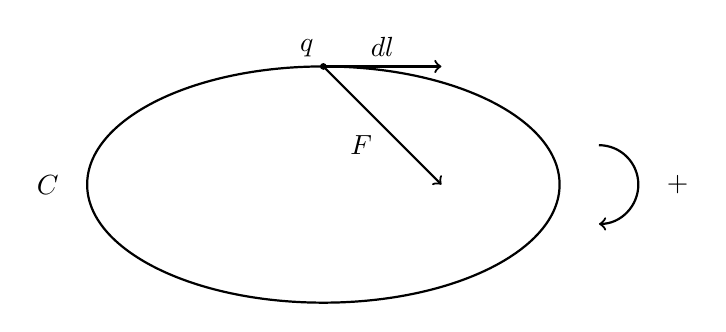
\begin{tikzpicture}
        % Draw the elliptical loop C
        \draw[thick] (0,0) ellipse (3cm and 1.5cm);
        
        % Label the loop C
        \node at (-3.5,0) {$C$};
        
        % Place the charge q and draw the vectors
        \filldraw (0,1.5) circle (1pt) node[above left] {$q$};
        
        % Draw dl vector
        \draw[->, thick] (0,1.5) -- (1.5,1.5) node[midway, above] {\(d \vb{l} \) };
        
        % Draw F vector
        \draw[->, thick] (0,1.5) -- (1.5,0) node[midway, below left] {\(\vb{F} \) };
        
        % Draw the circular arrow with a plus sign
        \draw[->, thick] (3.5,0.5) arc[start angle=90, end angle=-90, radius=0.5cm];
        \node at (4.5,0) {\(\boldsymbol{+} \) };
    \end{tikzpicture}
\end{center}

This formula is basically identical to the definition of work done, where \(W = \int_{a}^{b} \vb{F} \cdot d \vb{s}  \), just that we always perform loop integral for \(\mathcal{E}\) and the forces we use for calculating emf is per unit charge. Therefore, emf can also be interpreted as the work done by the net force per unit charge around a circuit.\footnote{This intepretation is flawed when the circuit itself is in motion. We will deal with this problem when discussing generators.}

There are really two force involved in driving charges around a circuit: the source force, \(q \vb{f} _{s}  \), which is usually confined to one portion of the loop (a battery, say) and an electromagnetic force, \(q(\vb{E} + \vb{v} \cross \vb{B} ) \), \textit{i.e.,} 

\begin{equation}
    \vb{f} = \vb{f} _{s} + \vb{E} . 
\end{equation}

The physical agency responsible for \(\vb{f} _{s} \)  can be many different things: in a battery it is a chemical force; in a piezoelectric crystal, mechanical pressure is converted into an electrical impulse; in a thermocouple it is a temperature gradient that does the job; in a photoelectric cell it is light; and in a Van de Graaff generator the electrons are literally loaded onto a conveyer belt and swept along. 

\subsection{Motional Emf}
\subsubsection{Flux Rule}
Consider a loop of wire moving inside a static magnetic field \(\vb{B} (\vb{r} )\). Let \(\vb{v} \) be the velocity of the element \(d \vb{l} \) relative to our inertial frame of reference (lab frame). Let \(\vb{u}\) be the velocity of \(q\) relative to \(C\), which must be directed along \(d \vb{l} \) since \(q\) cannot escape the wire in \(C\)'s frame. Thus the total velocity of \(q\) relative to us is \(\vb{v} _{\text{tot} } = \vb{v} + \vb{u} \). The force from the magnetic field on \(q\) is then

\begin{equation}
    \vb{F} = q(\vb{v} _{\text{tot} } \cross \vb{B} ) = q (\vb{v} \cross \vb{B} ) + q (\vb{u} \cross \vb{B} ).
\end{equation}

The emf of the circuit \(C\) is then 

\begin{equation}
    \mathcal{E} = \oint_{C} \vb{f} \cdot d \vb{l} = \oint_{C} (\vb{v} \cross \vb{B} ) \cdot d \vb{l}  + \oint_{C} (\vb{u} \cross \vb{B} ) \cdot d \vb{l} = \oint_{C} (\vb{v} \cross \vb{B} ) \cdot d \vb{l} ,
\end{equation}

where the term containing \((\vb{u} \cross \vb{B} )\cdot d\vb{l} \) vanishes since \(\vb{u}\) is parallel to \(d \vb{l} \). This is device is known as the generator and the emf is known as the ``motional emf'' since it is the emf produced from the motion of the loop.

Note that for this formula to apply, the loop of wire can have arbitrary and changing shape and the magnetic field can be non-uniform (but constant in time). 

If we consider two time instant \(t \text { and } t+dt\), then from \cref{ribbon} we can see that the change in magnetic flux is

\onefig{ribbon}{scale=0.3} 

\begin{equation}
    d\Phi = \Phi (t+dt) - \Phi (t) = \Phi _{\text{ribbon}} = \oint_{\text{ribbon} } \vb{B} \cdot d \vb{S} 
\end{equation}

since the magnetic field lines that pass through \(C\) at time \(t\) must either pass through \(C\) at time \(t+dt\) or the surface between them, which we denoted as \(S _{\text{ribbon} } \) (which is still a 2-D surface just that the ends of the surface overlap each other). 

The infinitisimal surface \(d \vb{S} \) in the above equation can be found if we focus on a certain point \(P \rightarrow P'\) which are the origin for the vector \(d \vb{l} \) at time \(t \text { and }  t+dt\) respectively, which corresponds to the area \(d\vb{S} = \vb{v} dt \cross d\vb{l} \) as shown in \cref{ribbon}. Thus, we have

\begin{equation}
    \frac{d\Phi }{dt} = \oint_{C} \vb{B} \cdot (\vb{v} \cross d \vb{l} ) = -\oint_{C} (\vb{v} \cross \vb{B} ) \cdot d \vb{l}.    
\end{equation}

Combining the results, we get the flux rule

\begin{equation} \label{motionalemf} 
    \mathcal{E} = \oint_{C} (\vb{v} \cross \vb{B} )\cdot d \vb{l} = -\frac{d\Phi }{dt}
\end{equation}

for the motional emf of a loop of wire moving in a static magnetic field.

It is important to understand that the flux rule is just a nifty shortcut for calculating motional emfs and the underlying principle is just the Lorentz force law. So for example when the switch in \cref{paraflux} is thrown from \(a\) to \(b\) although the flux \(\Phi \) is doubled, the motional emf \(\mathcal{E}\) is still zero, since there is no force driving the charges around (mathematically, in the derivation above we only assumed we have a single wire loop).

\onefig{paraflux}{scale=0.3} 

\subsubsection{Generator}

A Generator consists of a loop of wire \(C\) with a rectangular shape and is being pulled out of a region of magnetic field of strength \(\vb{B} = B \vu{z}  \) (into the page) at constant velocity \(\vb{v} = v \vu{x} \)  as shown in \cref{generator}.

\onefig{generator}{scale=0.3} 

The emf in this scenario is then 

\begin{equation}
    \mathcal{E} = \oint_{C} \vb{f}  \cdot d \vb{l} = \oint_{C} ((\vb{v} + \vb{u}) \cross \vb{B} ) \cdot  d\vb{l}  = \oint_{C}(\vb{v} \cross \vb{B} )\cdot d \vb{l} =  vBh ,
\end{equation}

where \(h\) is the width of the loop and \(\vb{u}\) is the velocity of the charge relative to the moving loop as always. Notice that the integral peformed to calculate \(\mathcal{E}\) is carried out at one instant of time (imaging taking a snapshot of the loop), thus \(d \vb{l} \) points straight up even though the loop is moving to the right.  

If we use the definition that the emf is the work done per unit charge around a loop (which is correct in most cases), then the above result shows that the magnetic force does work to the charge. However, magnetic force never does work. So what is wrong?

The problem is that this intepretation no longer works as the circuit itself is in motion. Since the infinitisimal displacement of charges would then not be equal to the infintisimal length element of the circuit, so \(d \vb{l} \) in emf is not equals to \(d \vb{s} \) in work done. When we are calculating the emf \(\mathcal{E}\), we are taking a snapshot of the loop and carry out the integral at a single instant. However, when we are calculating the work done \(W\) we are performing a path integral over time. In the case where the loop is stationary, the two integrals are equivalent and we can regard the emf as the work done by the force, \textit{i.e.,} \(\mathcal{E}= W\). 

To find the actual work done on an unit charge, we refer to \cref{genvel}, showing the velocities and the forces of a charge flowing through the loop, where the charge has a vertical velocity \(\vb{u}\) due to current in addition to the horizontal velocity \(\vb{v} \) due to the moving loop. Accordingly, the magnetic force per unit charge \(\vb{f} _{\text{mag} } \) has a horizontal component due to \(\vb{u}\) in addition to the vertical component due to \(\vb{v} \). An additional pulling force \(\vb{f} _{\text{pull} } \) is acted on the charge by the person pulling the rod.\footnote{More precisely, it is the rod that pulls the charges, but then the charges drags the rod due to Newton's second law, which is cancelled by the pulling force by the person. So equivalently, the person pulls the charges.}   

\onefig{genvel}{scale=0.3} 

\onefig{difpath}{scale=0.3} 

For the charge to move at a constant horizontal velocity with the loop (else it will not be confined in the loop), we must have 

\begin{equation}
    \vb{f} _{\text{pull} } = uB \vu{x} \implies \vb{f} _{\text{net} } = (\vb{f} _{\text{mag} })_{y} = vB \vu{y} . 
\end{equation}

So the actual work done on the charge is 

\begin{equation}
    W = \int \vb{f} _{\text{net} } \cdot d \vb{s} = vB \int \vu{y} \cdot d \vb{s} = vB\left( \frac{h}{\cos \theta }  \right)\cos \theta .
\end{equation}

It can also be interpret as the work done by the pulling force alone, since magnetic force do not work

\begin{equation}
    W = \int \vb{f} _{\text{net} } \cdot d \vb{s} =  \int \vb{f} _{\text{pull} } \cdot  d \vb{s} =  uB \left( \frac{h}{\cos \theta }   \right) \sin \theta  = vBh.
\end{equation}

As it turns out, the work done per unit charge is exactly equals to the emf, though the integrals are taken along entirely different paths (see \cref{difpath}). So in some sense, the emf can still be regarded as the work done per unit charge around a loop, just that the force responsible for establishing the emf (magnetic force in this case) may not be the same force that is responsible for the work done (pulling force by the person in this case).

In the loop, the charge is being accelerated continously by \(\vb{f} _{\text{net} } = vB \vu{y}  \), just as how it is accelerated in an ordinary battery, just that in this case the emf is not localized but span the whole length of the wire \(ab\) in \cref{difpath}.    

\subsection{Faraday's Law}

Consider now a closed wire \(C\) that is at rest inside a time-varying magnetic field \(\vb{B} (\vb{r} ,t)\). Experiments show that as soon as \(\vb{B} \) starts changing, a current begins to flow in the wire. This is weird as magnetic field should only act on moving charges, hence the only explanation is that a time-varing magnetic field induces an electric field \(\vb{E} (\vb{r} ,t)\).\footnote{``Induce'' is a subtle and slippery verb. It carries a faint odor of causation (“produce” would make this explicit) without quite committing itself. There is a sterile ongoing debate in the literature as to whether a changing magnetic field should be regarded as an independent “source” of electric fields (along with electric charge) -- after all, the magnetic field itself is due to electric currents. It is like asking whether the postman is the “source” of my mail. Well, sure -- he delivered it to my door. On the other hand, Grandma wrote the letter. Ultimately, \(\rho \)  and \(\vb{J} \)  are the sources of all electromagnetic fields (magnetic fields produced by a magnet also arises from the many internal currents (which is equivalent to a solenoid after the cancelation)), and a changing magnetic field merely delivers electromagnetic news from currents somewhere else. But it is often convenient to think of a changing magnetic field “producing” an electric field, and it will not hurt you as long as you understand that this is the condensed version of a more complicated story}
 
The emf of the circuit is now

\begin{equation}
    \mathcal{E} = \oint_{C} \vb{E} \cdot d \vb{l}.
\end{equation}

According to experiments, it turns out that the emf in this case can also be written in

\begin{equation}
    \mathcal{E}= - \frac{d\Phi }{dt}.
\end{equation}

Note that although this equation is identical to \cref{motionalemf}, the underlying mechanism is entirely different. In the motional emf case, the emf is established by magnetic force on the moving charges. Now, however, it is generated by the electric field induced by the changing magnetic field. At this stage, we should view the two cases separately although it is not a mere coincidence that the two equations are identical.

This result, on contrary to motional emf, can not be derived mathemtically, since it is in fact a physical law have been tested countless times. The negative sign on the RHS of the above equation expresses Len'z law, which states that states that the direction of the electric current induced in a conductor by a changing magnetic field is such that the magnetic field created by the induced current opposes changes in the initial magnetic field, but Lenz did not state the mathmatical relation of them. 

Writing \(\mathcal{E}\text { and } \Phi \) explicitly we have

\begin{equation}
    \oint_{C}\vb{E}  \cdot d \vb{l} = -\oint_{\mathcal{S}} \frac{\partial \vb{B} }{\partial t}\cdot d \vb{a} ,  
\end{equation}

This is the Faraday's law in integral form. Converting it to differential form by applying the Stoke's theorem, we get

\begin{equation}
    \curl{\vb{E} } = -\frac{\partial \vb{B} }{\partial t}.  
\end{equation}

If one would like, \(\partial \vb{B} /\partial t\) can be regarded as a current source for electric field, since the Faraday's law is mathematically identical to the Ampere's law, with \(\vb{E} \text { and } \vb{B} \) (and the divergence of both \(\vb{E} \text { and } \vb{B} \) are both zero for pure Faraday electric field, \textit{i.e.,} due exclusively to a changing \(\vb{B} \), with \(\rho =0\)) interchanged. We therefore have the Biot-Savart law for electric field 

\begin{equation}
    \vb{E} = -\frac{1}{4\pi } \frac{d}{dt} \int_{V}^{} \frac{\vb{B} \cross \hrcurs }{\rcurs ^2} d\tau .  
\end{equation}

However, this equation is seldom used since symmetries are usually present to avoid equation.




\section{Electromagnetic Induction and Magnetic Energy}

\subsection{Electromagnetic Induction}

Suppose you have two loops of wire, with current \(I_1 \text { and } I_2 \) producing magnetic field \(\vb{B} _{1} \text { and } \vb{B} _{2}\) respectively. From the Biot-Savart law, we can easily see that the magnetic field \(\vb{B} _{1} \) is proportional to the current \(I_1 \), so as the flux through loop 2 

\begin{equation} \label{Phi2} 
    \Phi _{21} = \oint_{S} \vb{B} _{1} \cdot d\vb{S} = M_{21} I_1 ,    
\end{equation}

where \(M_{21} \) is the constant of proportionality, known as the mutual inductance of the two loops (since, as we will see, \(M_{12} = M_{21}  \)). In fact, it can be found explicitly by

\begin{equation}
    \Phi _{21} = \oint_{S} \vb{B} _{1} \cdot d \vb{S} _{2} = \oint_{S} (\curl{\vb{A} _{1} }  ) \cdot d\vb{S} _{2} = \oint_{C_2 } \vb{A} _{1} \cdot d \vb{l} _{2} = \oint_{C_2 } \frac{\mu _{0} I_1  }{4\pi }\oint_{C_1 } \frac{d \vb{l} _{1} \cdot d \vb{l} _{2}  }{\rcurs },            
\end{equation}

so evidently

\begin{equation}
    M_{21} = \frac{\mu _{0} }{4 \pi } \oint_{C_1 }\oint_{C_2 } \frac{d \vb{l} _{1} \cdot d \vb{l} _{2} }{\rcurs }.     
\end{equation}

From the above equation we can see that the mutual inductance is a purely geometrical quantity, and is symmetrical to both loops, \textit{i.e.,} \(M_{21} = M_{12}  \), which means that the flux through 2 when we run a current \(I\) around 1 is identical to the flux through 1 when send the same current \(I\) around 2. Therefore, we can drop the subscripts and call them both \(M\).

So returning to \cref{Phi2}, the induced emf in loop 2 can be found by 

\begin{equation}
    \mathcal{E}_{21} = - \frac{d\Phi _{21} }{dt} = - M \frac{dI_1 }{dt}.  
\end{equation}

By a similar fashion, a changing current in loop 2 would also change the flux through loop 2, so we can define the self inductance of loop 2 as 

\begin{equation}
    L_2  = \frac{\Phi _{22}  }{I_2 }, 
\end{equation}

where the induced emf due to the changing current in loop 2 is now

\begin{equation}
    \mathcal{E}_{22} = - L\frac{dI_2 }{dt},  
\end{equation}

which is called the back emf.

The total induced emf in loop 2 is therefore

\begin{equation}
    \mathcal{E}_{2}   = \mathcal{E} _{21} + \mathcal{E}_{22} =  -M\frac{dI_1 }{dt}  - L \frac{dI_2 }{dt}.
\end{equation}

Similar to capacitance, to find \(M \text { or } L\), the standard procedure is to run a current through one of the loop and find the flux through the another loop in terms of this current. 

Since the positive sense of \(\Phi _{1} \) is defined by the direction of the thumb when using the right hand rule while the four other fingers are pointing towards the positive current \(I_1 \), \(\Phi_{1}  \) must increase when \(I_1 \) increase and vice versa, so \(L = \Phi _{1} /I_1  \) is an intrinsically positive quantity. However, an increase in current in loop 1 \(I_1 \) can produce a positive or negative flux in loop 2 \(\Phi _{2} \), depending on how the positive sense of current is defined in loop 2, so the mutual inductance \(M = \Phi _{2} /I_1  \) can be positive or negative depending on the winding sense. If they are wounded in the same sense on a cylinder then \(M > 0\), and if they are wounded in the opposite sense on a cylinder then \(M > 0\).  

Lenz's law, which is enforced by the minus signs in the above equations, dictates that the emf is in such a direction as to oppose any change in magnetic flux. Whenever you try to alter the current in a wire, you must fight against this the back emf due to the loop's self inductance. Inductance plays an analogous role in electric circuits that mass plays in mechanical systems: the greater \(L\) is, the harder it is to change the current, just as the larger the mass, the harder it is to change an object's velocity.

\example{Transformer.}
{Coil \(A\) is driven by a voltage of the form \(V = V_0 \sin (\omega t)\). Find the voltage across coil \(B\).  }
{The equation for coil \(A\) is 

\begin{equation}
    V_0 \sin (\omega t) = L_{A} \frac{dI_{A} }{dt}  
\end{equation}

} 


\example{Jumping Ring.}
{If you wind a solenoidal coil around an iron core (which serves to beef up the magnetic field), place a metal ring on top, and connect the coil with an AC source, the ring will jump in the air. Why? (The situation is illustrated in \cref{jumpingring}).}
{Before you turned on the current, the flux through the ring was zero. Afterward a flux appeared, and the emf generated in the ring led to a current (in the ring) which, according to Lenz’s law, was in such a direction that its field tended to cancel this new flux. This means that the current in the loop is opposite to the current in the solenoid. And opposite currents repel, so the ring flies off.} 
\onefig{jumpingring}{scale=0.3} 

\example{Magentic Forces do No Work (1).}
{Refer to \cref{nowork1}, we model a car made of ferromagnetic material as a circular current loop, since magnetization is the same as magnetic dipole is the same as current loop. For simplicity, we picture the current loop as a nonconducting ring of radius \(a\), line charge density \(\lambda \), rotating at angular velocity \(\omega\). Analyze why the magnetic force do not work despite it is the force responsible in lifting the car.  }
{The upwrd magnetic force on the loop is\footnote{Assume for now that the magnetic field remains constant as the loop rises. We will relax this assumption in the next example.} 

\begin{equation}
    F = 2\pi I a B_{\rho } = 2\pi \lambda \omega a^2B_{\rho } , 
\end{equation}

where \(B_{\rho } \) is the radial component of the magnetic field. 

The work done on it is 

\begin{equation}
    dW = 2\pi \lambda \omega a^2B_{\rho }dz. 
\end{equation}

The motional emf induced in the ring is

\begin{equation}
    \mathcal{E} = \oint_{C} \vb{f} \cdot d\vb{l} = - \frac{d\Phi }{dt} = -\frac{d}{dt} (B_{\rho } 2\pi a dz ) = -B_{\rho } \frac{dz}{dt},   
\end{equation}

where \(\vb{f} \) is the force per unit charge,\footnote{Note that \(\vb{f} \) here is not electric force but magnetic force since there is no changing magnetic field, so we are using the flux rule but not the Faraday's law.} and the magnetic flux \(\Phi \) is found by considering the ribbon joining the ring at time \(t\) to the ring at time \(t+dt\) (accompanied by the fact that \(\div{\vb{B} } = 0 \)).    

So the work done by the torque due to \(\vb{f} \) is 

\begin{equation}
    dW = Nd\phi = a\left( -B_{\rho } \frac{dz}{dt}   \right) \lambda (2\pi a)(\omega dt) = -2\pi \lambda \omega a^2B_{\rho }. 
\end{equation}

The ring slows down and the rotational energy it loses is precisely equal to the potential energy it gains. All the magnetic field did was to convert the rotational energy to gravitational potential energy, but did not provide extra energy to the system.

If one would permit some sloppy language, the work done by the vertical component of the magnetic force to raise the car is equal and opposite to the work done by its horizontal component to weaken the magnetization of the car.


} 

\twofig{nowork1}{height=5cm}{nowork2}{width=\textwidth}{nowork} 

\example{Magnetic Forces do No Work(2).}
{In the above example, we have assumed that the magnetic field remains unchanged during the car's ascend. Carry out similar analysis process as above and explain the role the magnet does during the process.}
{Refer to \cref{nowork2}, we model the magnet as a big circular loop of radius \(b\) resting on a table and carrying a current \(I_{b} \). At equilibrium, we have the magnetic force between the loops is 

\begin{equation}
    F_{\text{mag} } = m_{a}g  = \grad{(\vb{m} \cdot \vb{B} )} = \grad{\left( I_{a}\pi a^2 \frac{\mu_0 I_{b} }{2} \frac{b^2}{(b^2+z^2)^{\frac{3}{2} } }    \right)} = \frac{3\pi }{2} \mu_0 I_{a}I_{b}\frac{a^2b^2h}{(b^2+h^2)^{\frac{5}{2} } } .      
\end{equation}

When the loop rises an infinitesimal distance \(dz\), the increase in potential energy is 

\begin{equation}
    dU_{a}  = F_{\text{mag} } dz = \frac{3\pi }{2} \mu_0 I_{a}I_{b}\frac{a^2b^2h}{(b^2+h^2)^{\frac{5}{2} } }dz.     
\end{equation}

This energy is not provided by the magnetic field,\footnote{Straightly speaking, this work done is provided by the magnetic field, but the magnetic field also tries to do negative work by decreasing the current. So ultimately the power supply is the only source that provide energy to the system. It aims to increase the current but magnetic field steal this energy and put it as gravitational potential energy.} but by the power suppply that sustains the current in loop \(a\). As the loop rises, the motional emf induced in loop \(a\) is 

\begin{equation}
    \mathcal{E}_{a} = - \frac{d\Phi _{a} }{dt} = -I_{b} \frac{dM}{dt} = -I_{b}\frac{dM}{dt}\frac{dh}{dt} = -\frac{3\pi }{2} \mu_0 I_{b} \frac{a^2b^2h}{(b^2+h^2)^{\frac{5}{2} } }\frac{dz}{dt},          
\end{equation}

so the work done by the power supply fighting against this back emf is 

\begin{equation}
    dW_{a}  = -\mathcal{E}I_{a}dt = \frac{3\pi }{2}\mu_0 I_{a}I_{b}\frac{a^2b^2h}{(b^2+h^2)^{\frac{5}{2} } }dz,     
\end{equation}

which is the same as the work done in lifting the loop. If there is no power supply sustaining the current then the current will decrease, as in the previous example, where the angular velocity of the ring decreases.

The above calculation is essentially the same as the previous example, just that the magnetic field created by the upper loop is explicitly expressed. 

Meanwhile, a Faraday emf is induced in the upper loop due to the changing flux from the lower loop 

\begin{equation}
    \mathcal{E}_{b} = -I_{a}\frac{dM}{dt} = -\frac{3\pi }{2} \mu_0 I_{a}\frac{a^2b^2h}{(b^2+h^2)^{\frac{5}{2} } },      
\end{equation}

and the work done by the power supply fighting against this back emf is 

\begin{equation}
    dW_{b} = - \mathcal{E}I_{b}dt = \frac{3\pi }{2} \mu_0 I_{a}I_{b} \frac{a^2b^2h}{(b^2+h^2)^{\frac{5}{2} } }dz.      
\end{equation}

This work done is stored in the increasing magentic field n

\begin{equation}
    dU = d\left( \frac{1}{2}L_{a}I_{a}^2 = \frac{1}{2}L_{b}I_{b}^2 + MI_{a}I_{b}         \right) = I_{a}I_{b}\frac{dM}{dt}dt = dW_{b}.    
\end{equation}

If we care to apportion things this way, the power supply in loop \(a\) contributes the energy necessary to lift the lower ring, while the power supply in loop \(b\) provides the extra energy for the fields. If all we are interested in is the work done to raise the ring, we can ignoer the upper loop and the energy in the fields altogether, as in the previous example.
} 

\example{Magnetic Forces do No Work (3).}
{If, however, in more practical scenerio, the magnet stays in contact with the car, and the magent-car system is raised by a rope, then do we no power supply for the loops?}
{According to the apportion between work and energy established in the previous example, the upper loop need no power supply since the field energy remains unchanged. 

On the other hand, we need no power supply either for the lower loop since the work done against the back emf is provided by the pulling force. To illustrate this point, refer to \cref{nowork3}, where we increase the current \(I\) in the loop so that the magnetic force exceed s the weight and the loop rises. The velocities and the forces of the loop during its ascend are shown in \cref{nowork4}.

As the loop ascends, the magnetic force tilt back. While the vertical component is responsible for lifting the loop there must be } 

\twofig{nowork3}{width=\textwidth}{nowork4}{width=\textwidth}{noworknowork} 


\subsection{Magnetic Energy}

The energy stored inside an inductor as magnetic energy is given by 

\begin{equation}
    U = \int dW = \int -\mathcal{E}dq = \int LIdI = \frac{1}{2}LI^2. 
\end{equation}

Here the negative sign after the second equality is due to the fact that this is the work done by me against the back emf, not the work done by the emf.

In fact, this expression can be treated as the definition of the self-inductance \(\vb{L}\), sometimes when the current is not confined to a single path, it is easier to find the magnetic energy stored in the system for a current \(I\) then use the above equation to find the self-inductance \(L\).  

To generalize this expression, we note that 

\begin{equation}
    \Phi = LI = \int \vb{B} \cdot d\vb{S} = \int (\curl{\vb{A} } ) \cdot d\vb{S} = \oint_{C} \vb{A} \cdot d\vb{l},
\end{equation}

so the energy (or the work done by me) is 

\begin{equation}
    \begin{aligned} 
    U &= \frac{1}{2} I \oint_{C} \vb{A} \cdot d\vb{l}   = \frac{1}{2} \oint_{C} (\vb{A} \cdot \vb{I} )d\vb{l} = \frac{1}{2} \int_{V}^{} (\vb{A} \cdot \vb{J} )d\tau = \frac{1}{2\mu_0 } \int_{V}^{} \vb{A} \cdot (\curl{\vb{B} } )d\tau \\
    &= \frac{1}{2\mu_0 }\int_{V}^{} \left( B^2-\div{(\vb{A} \cross \vb{B} )}  \right) d\tau = \frac{1}{2\mu_0 } \int_{\text{all space} }^{} B^2d\tau ,    
    \end{aligned}   
\end{equation}

where the second term in the integrand vanishes when we take the volume to be all space, since \(\vb{J} \) is zero outside the volume occupied by the current anyways, so it won't contribute to any extra magnetic energy. 

\section{Maxwell's Equations}

\subsection{Displacement Current} \label{displacement} 

Before we group the four Maxwell's Equations we have found, there is a small (but important) final modification to the Ampere's law, motivated by the fact that if we take the divergence of the Ampere's law we get

\begin{equation}
    \div{(\curl{\vb{B} } )} = \mu_0 \div{\vb{J} } = -\mu_0 \frac{\partial \rho }{\partial t} = -\div{\left( \epsilon_0 \frac{\partial \vb{E} }{\partial t}  \right)}, 
\end{equation}

where while the LHS must be zero since it is a divergence of a curl, the RHS is generally non-zero. The only remedy is to introduce the displacement current \(\vb{J} _{d} \)

\begin{equation}
    \vb{J} _{d} = \epsilon_0 \frac{\partial \vb{E} }{\partial t}, 
\end{equation}

and add this to the ordinary current density \(\vb{J} \), so that 

\begin{equation}
    \div{(\curl{\vb{B} } )} = \mu_0 \div{(\vb{J} + \vb{J} _{d} )} = -\div{\left( \epsilon_0 \frac{\partial \vb{E} }{\partial t}  \right)} + \div{\left( \epsilon_0 \frac{\partial \vb{E} }{\partial t}  \right)} = 0. 
\end{equation}

Therfore, the complete modified Ampere's law is 

\begin{equation}
    \curl{\vb{H} } = \vb{J}_{f} + \frac{\partial \vb{P} }{\partial t} + \epsilon_0 \frac{\partial \vb{E} }{\partial t} = \vb{J} _{f} + \frac{\partial \vb{D} }{\partial t}.      
\end{equation}

To summarize, we spilt the current density \(\vb{J} \) into four terms: the free current \(\vb{J} _{f} \), the bound current \(\vb{J} _{b} \), the polarization current \(\vb{J} _{p} \) and an extra artificial displacement current \(\vb{J} _{d} \) to obtain this final form.     

\example{Current without Magnetic Field.}
{Consider two concentric metal spherical sheels with inner and outer radius \(\vb{a} \text { and } \vb{b} \) respectivley. The inner shell carries a charge \(Q(t)\) while the outer one carries an opposite charge. The space between them is filled with an ohmic material of conductivity \(\sigma \), find the magnetic fields.   }
{This configuration is spherically symmetrical, so the magnetic field can only be raidal. However, from the Gauss's law for magnetism, we have 

\begin{equation}
    \div{\vb{B} } =0 \implies \oint_{S} \vb{B} \cdot d\vb{S} = 4\pi r^2B = 0 \implies B=0.
\end{equation}

So the magnetic field is zero everywhere, which is due to the fact that the actual current density \(\vb{J} \) cancels out with the displacment current density \(\vb{J} _{b} \).

The actual current density \(\vb{J} \) is 

\begin{equation}
    \vb{J} = \sigma \vb{E} = \frac{1}{4\pi \epsilon_0} \frac{\sigma Q}{r^2}\vu{r}, 
\end{equation}

while the displacement current is 

\begin{equation}
    \vb{J} _{b} = \epsilon_0 \frac{\partial \vb{E} }{\partial t} = \frac{1}{4\pi } \frac{I}{r^2}\vu{r} = \frac{1}{4\pi r^2}\left( \int \vb{J} \cdot d\vb{S} \right)\vu{r} = -\frac{1}{4\pi \epsilon_0} \frac{\sigma Q}{r^2}\vu{r} = -\vb{J} . 
\end{equation}
}

\subsection{Maxwell's Equations and Boundary Conditions}

The Maxwell's equations are, in differential forms,

\begin{equation}
    \boxed{
    \begin{aligned}
        \div{\vb{E} } &= \frac{\rho }{\epsilon_0 } ,\\
        \curl{\vb{E} } &= -\frac{\partial \vb{B} }{\partial t},\\
        \div{\vb{B} } &= 0,\\
        \curl{\vb{B}} &= \mu_0 \vb{J} + \epsilon_0 \mu_0 \frac{\partial \vb{E} }{\partial t}.     
    \end{aligned}}
\end{equation}

In integral forms, they are 

\begin{equation}
    \boxed{
    \begin{aligned}
        \oint_{S} \vb{E} \cdot d\vb{S} &= \frac{Q_{\text{enc} } }{\epsilon_0 } ,\\
        \oint_{C} \vb{E} \cdot d\vb{l} &= - \frac{d}{dt} \int_{S}^{} \vb{B} \cdot d\vb{S}   ,\\
        \oint_{S} \vb{B} \cdot d\vb{S} &= 0 ,\\
        \oint_{C} \vb{B} \cdot d\vb{l} &= \mu_0 I_{\text{enc} } + \epsilon_0 \mu_0 \frac{d}{dt} \int_{S}^{} \vb{E} \cdot d\vb{S}     .     
    \end{aligned}}
\end{equation}

In polarized or magnetized materials, however, the modified forms of the Maxwell's equations might be more convenient. In differential forms,

\begin{equation}
    \boxed{
    \begin{aligned}
        \div{\vb{D} } &= \rho _{f},\\
        \curl{\vb{E} } &= -\frac{\partial \vb{B} }{\partial t},\\
        \div{\vb{B} } &= 0,\\
        \curl{\vb{H} } &= \vb{J} _{f} + \frac{\partial \vb{D} }{\partial t}.     
    \end{aligned}}
\end{equation}

In integral forms, they are 

\begin{equation} \label{boundary} 
    \boxed{
    \begin{aligned}
        \oint_{S} \vb{D} \cdot d\vb{S} &= Q_{f_{\text{enc} } } ,\\
        \oint_{C} \vb{E} \cdot d\vb{l} &= - \frac{d}{dt} \int_{S}^{} \vb{B} \cdot d\vb{S}   ,\\
        \oint_{S} \vb{B} \cdot d\vb{S} &= 0 ,\\
        \oint_{C} \vb{H} \cdot d\vb{l} &= I_{f_{\text{enc} } } + \frac{d}{dt} \int_{S}^{} \vb{D} \cdot d\vb{S}     .     
    \end{aligned}}
\end{equation}

The differential forms are easier for derivation while the integal forms are more convenient for applications. The ordinary Maxwell's equations are more classical and are more general while the modified equations are more used for applications.

The 4 corresponding boundary conditions are 

\begin{equation}
    \boxed{
    \begin{aligned}
        \epsilon _{\text{above} }E_{\text{above} }^{\perp } - \epsilon _{\text{below} }E_{\text{below} }^{\perp } &= \sigma _{f} ,\\
        B_{\text{above} }^{\perp } - B_{\text{below} }^{\perp } &=0,\\
        \vb{E} _{\text{above} }^{\parallelsum} - \vb{E} _{\text{below} }^{\parallelsum} &= \boldsymbol{0} ,\\
        \frac{1}{\mu _{\text{above} } }\vb{B} _{\text{above} }^{\parallelsum} - \frac{1}{\mu_{\text{below} } }\vb{B} _{\text{below} }^{\parallelsum} &=\vb{K} _{f}\cross \vu{n}  .                    
    \end{aligned}
    }
\end{equation}

\chapter{Circuit Theory}

\section{Electromotive Force, Potential Difference and Voltage}

Before dealing with any circuit components, it is important to distinguish between 3 very similar quantities:

\begin{enumerate}
    \item Electromotive force (emf) (\(\mathcal{E}\)): 

    Emf of a circuit element is the loop integral of the force provided by the circuit element (emf source) per unit charge, which is also equivalent to the work done by the emf source to charges per unit charge per loop. This is generally non-zero, meaning that the force is non-conservative.
    
    Emf of a circuit also make sense to say, which is simply the sum of all individual emf from every emf source.

    Battery and inductor are examples of emf sources, where the source force is a constant ``chemical force'' and a non-conservative electric force, respectively. A more detailed discussion on emf can be refered to the dedicated section \cref{emf}. 

    \item Potential difference (\(\Delta V\)): 
    
    Potential difference is only well-defined for conservative electric field, as the negative of the conservative electric field line integral, which is equivalent to the negative work done by the electric field per unit charge.
    
    For non-conservative electric field the potential difference between two points is ill-defined since the line integral is path dependent so there is no unique answer. 

    Therefore, since the electric fields in a resistor, capacitor and battery are conservative (generated by static charges), the potential differences across them is well defined. However, we cannot define a potential difference across an inductor since the electric field in an inductor is non-conservative. We will discuss more on this in \cref{elec}. 

    \item Voltage (\(V\)): 
    
    Voltage is a general term used exclusively in circuit theory to refer to both the potential difference and emf. As we will show, the voltage at each point of a circuit is well-defined (as long as the ground (the point where the voltage is defined to be zero)) is given.
\end{enumerate}

\section{Circuit Elements}

Before analyzing any circuit, it is useful to first understand basic properties of the 4 main cirucit elements, they can be calssified into active circuit elements (or emf sources), which are those that can supply energy to a circuit, or passive circuit element, which are those that cannot generate energy but instead store, release or dissipate energy supplied by the active elements:

\begin{enumerate}
    \item Battery (\(\mathcal{E} = \mathcal{E}_{0} \)): An emf source where the source force is a ``chemical force'', pointing from the negative terminal to the positive terminal, thus an active circuit element.
    \item Resistor (\(\Delta V = -IR\)): Disspate energy via collisions between charges and positive ions inside the resistor as heat, thus a passive circuit element.
    \item Capacitance (\(\Delta V = -q /C \)): Store and release energy via electric field, thus a passive circuit element.
    \item Inductor (\(\mathcal{E} = -L(dI /dt) \text { or } \Delta V = L(dI /dt)\)): An emf source where the source force is an electric force, pointing along the curled wire. Due to the negative sign as enforced by Len'z law, an inductor would always oppose the change in curerent and is not capable of generating energy. Therefore, instead of intepretaing an inductor as an emf source (which pushes charges along the circuit) with negative emf (which is also valid), we usually intepret it as a passive circuit element, which store and release energy via magnetic field.   
\end{enumerate}

The generic equation of any circuit is 

\begin{equation}
    \text{Energy provided to the circuit} = \text{Energy consumed by the circuit},
\end{equation}

or equivalently, 

\begin{equation} \label{energycircuit} 
    \sum_{\text{loop} }^{} \mathcal{E} = \sum_{\text{loop} }^{} \Delta V. 
\end{equation}

So we can define voltage as \(V = \mathcal{E}\) for emf sources or \(V = \Delta V\) for passive circuit elements such that 

\begin{equation}
    \sum_{\text{loop} }^{} V = 0 
\end{equation}

and thus \(V\) is well-defined and unique at every point in a circuit provided that ground (point of zero voltage) is defined prior.

In the case of a LRC circuit, this equation would be transformed to 

\begin{equation}
    \mathcal{E}_{0} - L\frac{dI}{dt} = IR + \frac{q}{C} \text {  ~~ or  ~~ } \mathcal{E}_{0} = IR + \frac{q}{C} + L\frac{dI}{dt} .  
\end{equation}

\section{Electric Fields in Circuits} \label{elec} 

To understand the operation of circuit fully, we have to connect to the theory of electromagnetism and apply it here. 

The electric fields involved in circuits can be separated into two categories: conservative (due to static charges) and non-conservative (due to changing magnetic field).

For every circuit elements in a circuit, there has to be an associated electric field which is related to the potential difference across the element or the emf of the element:

\begin{enumerate}
    \item Battery: Assuming the battery is ideal (\textit{i.e.,} the internal resistance is negligible), we can take \(\sigma \rightarrow \infty\) and \cref{ohm} tells us that the net force experienced by a charge inside the battery is zero. (This fact can be extended more generally by arguing that when the current is constant, the speed of the charge is constant, so the net force experienced by the charge at every point in the circuit is zero.) This implies that there will be an electric field with the same magnitude and opposite direction as the source force. This electric field is conservative and is established by the accumlation of charges on the two ends of the battery.
    \item Resistor: Now that we cannot take \(\sigma \rightarrow \infty\), but then the electric field inside a resistor is straightforwardly given by \cref{ohm} as \(\vb{E} = \vb{J} /\sigma  \). This electric field cancel out with the ``resistive force'' due to collisions between the charge and the positive ions in the resistor, so that the net force experienced by the charge is still zero. The electric field in this case is also conservative and is established by the accumulation of charges on the two ends of the resistor.
    \item Capacitance: In some sense, a capacitor is essentially a resistor with zero resistance so no energy get lost as heat during collision but are instead stored in electric field. The electric field is still conservative and is established by the charges present on the plates. 
    \item Inductor: Now that the electric field is not due to static electric charge but by changing magnetic field, the electric field is no longer conservative. It would still be directed along the wire but since the wire is coiled, the electric field will have this coiling pattern as well. As the force on the charges is not zero, the current is no longer constant. It is exactly this effect that slows down the change in current, which is what makes an inductor an inductor.
\end{enumerate}

When we consider the emf of the circuit, we take the loop integral of the total force per unit charge. As every electrostatic field is curless, the work done by the electric field in the resistor, capacitor and battery all sum up to zero, which left the only work done to be the contribution of the source force and the electric field of the inductor. This is the LHS of \cref{energycircuit}. The RHS is then explaining where this energy go. It goes to heat in the resistor (or equivalently, work done against the resistive force) and energy stored in electric fields in capacitor. 

\section{Circuit with Battery and Resistor}

Consdier the following circuit consisting of a battery and a resistor:

\begin{center}
    \begin{circuitikz}
        % Draw the resistor and label current I
        \draw (1.5,0) to[R] (4.5,0);
        \draw[->] (3.5, 0.5) -- (2.5, 0.5) node[midway, above] {\(I \) };
        
        % Draw the top wire
        \draw (0,0) -- (1.5,0);
        \draw (4.5,0) -- (6,0);
        
        % Draw the right wire and arrows
        \draw (6,0) -- (6,-3);
        
        % Draw the battery with terminals a and b
        \draw (6,-3) to[battery] (0,-3);
        \filldraw (1.5,-3) circle (1pt) node[above] {\(a\) };
        \filldraw (4.5,-3) circle (1pt) node[above] {\(b\) };
        \node at (3.5,-3.2) {\(+\) };
        \node at (2.5,-3.2) {\(-\) };
        
        % Draw the bottom wire and label current I
        \draw (0,-3) -- (0,0);
        
        % Draw electric field vector E
        \draw[->] (4,-3.5) -- (2,-3.5) node[midway, below] {\(\vb{E} \) };
        \draw[->] (4,-0.5) -- (2,-0.5) node[midway, below] {\(\vb{E} \) };

        % Draw vector f0 in the middle
        \draw[->] (2.5, -2.5) -- (3.5, -2.5) node[midway, above] {\(\vb{f} _{s} \) };
    \end{circuitikz}
\end{center}

While to calculate the emf we have to measure the force per unit charge at every position of the circuit simulataneously, but since we are dealing with a static (time-independent) situation, we can imagine a single charge \(q\) making a complete tour around \(C\). The force per unit charge is then the combination of contribution from the source force \( \vb{f} _{s}    \) and the electric force \(q\vb{E}    \), so \(\vb{f} = \vb{f} _{s} + \vb{E}\) and the emf becomes

\begin{equation}
    \mathcal{E}= \oint_{C} \vb{f} \cdot d \vb{l} = \oint_{C} \vb{f}_{s}  \cdot d \vb{l} + \oint_{C} \vb{E} \cdot d \vb{l} = \oint_{C} \vb{f} _{s} \cdot d \vb{l} = \int_{a}^{b} \vb{f} _{s} \cdot d \vb{l}           
\end{equation}

since \(\oint_{C} \vb{E} \cdot d \vb{l} =0 \) for all electrostatic field and \(\vb{f} _{s} \) is non-zero only inside the battery. 

Now since the current \(I\) is constant, the charge \(q\) moves at constant speed along the circuit, which means that the total force on \(q\) in the direction of the path \(C\) is zero. In the interior of the resistor, the electrostatic force \( q\vb{E}  \) which arises from Ohm's law, is counterbalanced by the ``force'' on \(q\) due to the collision of the charges with the positive ions of the metal. In the battery, assuming the internal resistance is zero, there must be an electric field opposing the soruce force so \(\vb{E} = - \vb{f} _{s} \). This is also consistent to the fact that \(\vb{E} \) is curless around the circuit and \(\vb{f} = \vb{f} _{s} + \vb{E}  \) in \cref{ohm} should be zero if \(\sigma \rightarrow \infty\). 

The potential difference between the terminals is therefore 

\begin{equation}
    \Delta V = -\int_{a}^{b} \vb{E} \cdot d \vb{l} = \int_{a}^{b} \vb{f} _{s} \cdot d \vb{l} = \mathcal{E},
\end{equation}

which makes qualitative sense because the electromotive force is meant to push the charges up the potential hill.

The work done by the source force is then 

\begin{equation}
    W = \int_{a}^{b} q \vb{f} _{s} \cdot d \vb{l} = q \mathcal{E} = q\Delta V.
\end{equation}

In general, the energy gained by a charge \(q\) across a circuit element is given by 

\begin{equation}
    W = qV,
\end{equation}

where \(V\) is the voltage difference between two ends of a circuit element. If the difference is negative (with respect to the positive direction of the cirucuit loop), then enegy is lost instead of gained.

Current in this electric circuit is somewhat analogous to the flow of water in a closed system of pipes, with gravity playing the role of the electrostatic field, and a pump (lifting the water up against gravity) in the role of the battery. In this story, height is analogous to voltage.

\section{Sign Conventions}

To analyze any circuit, we have to first define a positive direction of each loop. The positive direction (terminal) of an emf is defined such that charges will be pushed along the positive direction of the loop while the positive direction (terminal) of passive circuit elements is reversed (this is called the passive sign convention). This is consistent to how charges accumulate on the ends of resistor, capacitor and battery and thus correctly show the direction of electric field and voltage change across circuit elements. The most standard RLC circuit is shown below:



\begin{center}
    \begin{circuitikz}
        \draw (0,0) to[battery, invert, l_=\(\mathcal{E}_{0} \)] (8,0) to[R, v=\(R\)] (8,5) to[L, v=\(L\)] (0,5) to [C, v=\(C\)] (0,0);
        \node at (2, -0.25) {\(-\) }; \node at (6,-0.25) {\(+\) };
        \draw[->, thick] (4,1.75) arc[start angle=-90, end angle=180, radius=0.75]; \node at (4,2.5) {\(I\) };
        \draw[->] (7.5,1.5) -- (7.5,3.25) node[midway, left] {\(\vb{E} _{R} \) };
        \draw[->] (0.75,3.25) -- (0.75,1.5) node[midway, right] {\(\vb{E} _{C} \) };
        \draw[->] (5.25,0.5) -- (2.75,0.5) node[midway, above] {\(\vb{E} _{s}\) };
        \draw[->, bend left=30] (8.75,3.6) to node[midway, right] {\(V_{R} \) } (8.75,1.4);
        \draw[->, bend left=30] (-0.75,1.4) to node[midway, left] {\(V_{C} \) } (-0.75,3.6);
        \draw[->, bend left=15] (2.15,5.75) to node[midway, above] {\(V_{L} \) } (5.85,5.75);
        \draw[->, bend right=15] (2.15,-0.75) to node[midway, below] {\(V_{s} \) } (5.85,-0.75);
        \draw[->, thick, decorate, decoration={coil, aspect=0.5, segment length=4mm, amplitude=2mm}] (5.75,4.5) -- (2.25,4.5) node[midway, below, yshift=-3mm] {\(\vb{E} _{L} \) };
    \end{circuitikz}
\end{center}

From the figure, it becomes obvious why

\begin{equation}
    V_{s} = V_{R} + V_{L} + V_{C}.     
\end{equation}

If one were to ever confused with signs, simply imagine the voltages as ``voltage vectors'' drawn above, then \(\sum_{\text{loop} }^{} \vb{V} = 0 \) becomes easier to understand. 

Things can get tricky when there is more than one loop. Consider the circuit below:

\begin{center}
    \begin{circuitikz}
        \draw (0,0) to[battery, invert, l_=\(\mathcal{E}_{0} \)] (0,5) to[R, v=\(R\)] (5,5) to[C, v=\(C\)] (5,0) -- (0,0);
        \draw (5,5) -- (10,5) to[L, v=\(L\)] (10,0) -- (5,0);
        \node at (-0.25, 1.25) {\(-\) }; \node at (-0.25,3.75) {\(+\) }; \node at (5.25, 1.25) {\(+\) }; \node at (5.25, 3.75) {\(-\) };
        \node at (5.25, 2) {\(-q\) }; \node at (5.25,3) {\(+q\) };
        \draw[->, thick] (1.5,2.5) arc[start angle=180, end angle=-90, radius=0.75]; \node at (2.25,2.5) {\(I_1 \) };
        \draw[->, thick] (7,2.5) arc[start angle=180, end angle=-90, radius=0.75]; \node at (7.75,2.5) {\(I_2 \) };
        \draw[->, bend left=30] (4.25,1.35) to node[midway, left] {\(V_{C_1 } \) } (4.25,3.6);
        \draw[->, bend left=30] (5.75,3.6) to node[midway, right] {\(V_{C_2 } \) } (5.75,1.35);
    \end{circuitikz}
\end{center}

In this circuit, the terminals of the capacitor has opposite polarities in the two loops. This is fine, however, as long as we separetely define the charge on the capacitor clearly, so the charge on the capacitor and the current is related by

\begin{equation}
    I_1 - I_2 = \frac{dq}{dt} .
\end{equation}

And the two circuit equations for the two loops are

\begin{equation}
    \mathcal{E}_{0} = I_1 R + \frac{q}{C} \text { ~~ and ~~ } 0 = L\frac{dI_2 }{dt} - \frac{q}{C}    
\end{equation}

Again, if we view \(V_{C_1 } \text { and } V_{C_2 } \) as vectors, it becomes clear why there is a negative sign for the second circuit equation above. This is becasue \(V_{C_1 } = q /C = -V_{C_2 }\). 

Sometimes, instead of loop current, we define different currents for each separate wire segment. Sometimes the equations are easily to solve this way, but then note that when writing down the loop equation a minus sign should be added if the current's pre-defined direction is opposite to how you are trasversing the loop.

\section{LRC Circuits}

The standard equation for LRC circuit is 

\begin{equation}
     L\frac{d^2q}{dt^2} + R\frac{dq}{dt} + \frac{q}{C} = \mathcal{E}_{0}\cos (\omega t + \varphi ) 
\end{equation}

The standard way of solving this form of diffrential equation is detailed in the ``Differential Equations'' notes, in which we would consider it as the real part of the copmlex differential equation

\begin{equation}
    L\frac{d^2\tilde{q} }{dt^2} + R\frac{d\tilde{q} }{dt} + \frac{\tilde{q} }{C} = \tilde{\mathcal{E}_{0} }e^{i \omega t},  \quad q = \mathfrak{Re} (\tilde{q} ) ~\text { and }~ \tilde{\mathcal{E}_{0} } = \mathcal{E}_{0} e^{i \varphi },
\end{equation}

where the standard guess for particular solution is 

\begin{equation}
    \tilde{q}  = \tilde{q_0 }e^{i \omega t} \implies \tilde{I} = \frac{d \tilde{q} }{dt} = i \omega \tilde{q_{0} } e^{i \omega t} = \tilde{I_0 }e^{i \omega t}.    
\end{equation}

which upon substitution gives 

\begin{equation}
    \left( L\omega ^2 + i \omega R + \frac{1}{C}  \right) \tilde{q_0 } = \tilde{\mathcal{E}_{0} }.
\end{equation}

Dividing both sides by \(\tilde{I_{0} } = i \omega \tilde{q_{0} } \) gives 

\begin{equation}
    i \omega L + R + \frac{1}{i \omega C} = \frac{\tilde{\mathcal{E}_{0} } }{\tilde{I_{0} } }, ~\text { or }~ \tilde{I_{0} }(Z_{L} + Z_{R} + Z_{C}  ) = \tilde{\mathcal{E}_{0} }.  
\end{equation}

and can be added in parallel or in series like ordinary resistors. 

The essential idea is that when there is a sinusoidal driving voltage of frequency \(\omega \), since we have neglected the homogeneous solution and other particular solution we assume that all the possible voltages \(V\) and currents \(I\) are also oscillating with the same frequency \(\omega \) but possibly with a phase shift.

Therefore it is convenient to introduce the notion of complex voltage \(\tilde{V} \) and complex current \(\tilde{I} \), which satisfy 

\begin{equation}
    V = \mathfrak{Re} (\tilde{V} ) = \mathfrak{Re} (\tilde{V}_{0}  e^{i \omega t} ) ~\text { and }~ I = \mathfrak{Re} (\tilde{I} ) = \mathfrak{Re} (\tilde{I}_{0} e^{i \omega t}  ).    
\end{equation}

The complex impendances \(Z_{L}, Z_{R} \text { and } Z_{C}  \) of an inductor, resistor or capactior then relates the amplitudes and phases of by \(\tilde{V}  \text { and }  \tilde{I}\) via the ``complex Ohm's law''

\begin{equation}
    \tilde{V} = Z \tilde{I},
\end{equation}

which has both the information in the magnitude and phase.

The power supply to a circuit element is 

\begin{equation}
    P = \mathfrak{Re} (\tilde{I} )\mathfrak{Re} (\tilde{V} ),
\end{equation}

but we cannot define a ``complex power'' \(\tilde{P} = \tilde{I} \tilde{V}   \), and say \(P = \mathfrak{Re} (\tilde{P} ) \). This is because \(\mathfrak{Re} (\tilde{I} \tilde{V}  ) \neq \mathfrak{Re} (\tilde{I} ) \mathfrak{Re} (\tilde{V} )  \). Instead, we have 

\begin{equation}
    P = V_0 \cos (\omega t) I_0 \cos (\omega t+ \varphi _{\text{rel} } ) \implies \avg{P} = \frac{1}{2}V_0 I_0 \cos (\varphi _{\text{rel} }) = V_{\text{rms} }I_{\text{rms} }\cos (\varphi _{rel}),
\end{equation}

or in terms of current alone,

\begin{equation}
    P = I_0 ^2 \cos ^2(\omega t) R \implies \left \langle {P} \right \rangle = \left \langle {I^2} \right \rangle R = I_{\text{rms} }^2R = \frac{1}{2} I_0 ^2R . 
\end{equation}

This is the reason why inductor and capacitor cannot dissipate energy since \(V \text { and } I\) of them are \(\pi /2 \) out of phase, so the avergae power over time is zero.  

It is also important to note that this method only finds the particular solution, but not the homgenous one.

\example{Principles of Inductors.}
{Refere to \cref{inductor}, and find \(V_{A} \text { and } V_{B}  \) right after the switch is opened.}
{Before the switch is opened, \(V_{A} = V_{B} = 0\), and the current passes through the inductor is \(I_{L} = V_0 /R  \), since the inductor behaves essentially like a wire. After the swtich is opened, \(V_{A} = V_{0}  \) is trivial and since the current passes through the inductor is still \(I_{L} = V_0 /R  \), because the current must change continuously over an inductor, and therefore \(V_{B} = V_{A} + I_{L}R_2 = V_{0} \left( 1+ \frac{R_2 }{R_1 }  \right)   \).   } 

\onefig{inductor}{scale=0.5} 

\example{Infinite Network.}
{Refer to \cref{infnet}, and find \(V_{n} \text { and } I_{n}  \) in terms of \(V_1 \text { and } V_1 \).}
{The recursive relations of \((V_{n+1}, I_{n+1}) \text { and } (V_{n}, I_{n})\) for a general \(n\) are

\begin{equation}
    V_{n+1} = V_{n} - I_{n}Z ~\text { and }~ I_{n+1} = I_{n} - V_{n+1}Y.      
\end{equation}

Writing in matrix form,

\begin{equation}
    \begin{pmatrix}
         V_{n+1}  \\
         I_{n+1}  \\
    \end{pmatrix} = \begin{pmatrix}
        1 & -Z   \\
        -Y & 1+YZ  \\
    \end{pmatrix} \begin{pmatrix}
         V_{n}  \\
         I_{n}  \\
    \end{pmatrix}.
\end{equation}

Thus 

\begin{equation}
    \begin{pmatrix}
         V_{n}  \\
         I_{n}  \\
    \end{pmatrix} = \begin{pmatrix}
        1 & -Z  \\
        -Y & 1+YZ  \\
    \end{pmatrix}^{n} \begin{pmatrix}
        V_{1}  \\
        I_{1}  \\
   \end{pmatrix}.
\end{equation}



} 

\onefig{infnet}{scale=0.2} 

\example{Maxwell's Bridge.}
{A Maxwell's bridge circuit is shown in \cref{maxwell}. Find the unknown inductance and resistance \(L_{x} \text { and } R_{x}  \) and state the advantages of this bridge circuit. What practical alterations to the bridge shown in the figure would allow the measurements to be made? if the bridge is found to be far from the balance point when the component is inserted?}
{When the bridge is balanced, \textit{i.e.,} the voltmeter (or ammeter) at the center of bridge across the nodes (not shown in the figure) has zero reading, so we have 

\begin{equation}
    \frac{Z_{x}}{R_3 } = \frac{R_2 }{Z_{1} }, \quad Z_{x} = R_{x} + i \omega L_{x} \text { and } Z_1 ^{-1} = R_1 ^{-1} + (\frac{1}{i \omega C} )^{-1} ,      
\end{equation}

which gives 

\begin{equation}
    R_{x} = \frac{R_2 R_3 }{R_1 } ~\text { and }~ L_{x} = R_2 R_3 C.   
\end{equation}

Because we are measuring the zero crossing by adjusting the bridge's variable elements, rather than a large absolute signal, null detection gives much higher sensitivity and accuracy. Also, the measurement is indepedent of freqeuncy and we can determine both \(R_{x} \text { and } L_{x}  \) independently in a single set up. Further, any small resistance in the detector branch does not affect the null condition since at perfect balance the diagonal branch carries essentially zero current. Lastly the balance condition is also independent of the voltage source's impedance.

If the bridge is far from balance we can add a variable resistor in series with \(R_2 \) (or \(R_3 \)) so that the real part ratio can be coarsely tuned towards balance, we can also add a variable capacitor in parallel with \(R_1 \) so the imaginary part ratio can be adjusted. 
} 

\onefig{maxwell}{scale=0.3} 

\example{Bridge Circuit.}
{For the bridge circuit shown in \cref{bridge}, \(Z\) comprises of a resistor \(R_{x} \) parallel with a capacitor \(C_{x} \). Asumming that the bridge is balanced when the variable resistor \(R_{v} = R_{0} \) and when the angular frequency \(\omega = \omega _{0} \). Find the voltage at the ammeter in terms of the driving amplitude \(V_0 \) for \(\omega  = 0, \omega = \omega _{0}  \text { and as } \omega \to \infty \).        }
{The key point to note is that in a null-bridge measurement the ``ammeter'' is used as a null detector, not as a low-impedance ammeter in the usual sense. So for all purposes we can treat the ``ammeter'' as an open circuit, or a voltmeter. Otherwise if there is any non-zero voltage difference across the usual sense ammeter we would get infinite current.

Therefore for all \(\omega \) the left node always has voltage \(V_0 /2\). And for \(\omega = 0\) the capacitor acts as an open circuit while for \(\omega \to \infty\) the capacitor acts as a short circuit. In both cases the voltage at the left node is \(V_0 \), so the voltage difference is \(V_0 /2\). While for \(\omega = \omega _{0} \) the voltage difference is zero by the definition of \(\omega _{0} \).       } 


Practically speaking since there are parasitic winding capacitance in an inductor the frequency cannot be too large. Particularly if we model an inductor as a pure inductor \(L\) in parallel with its parasitic capacitance \(C\) the impedance would be \(Z = (i (\omega C - 1/\omega L))^{-1} \), which deviates from \(i \omega L\) if \(\omega \sim \frac{1}{\sqrt{LC} } \). However the frequency cannot be too small in some cases that the balance equation would require some extremely large capcitance to balance.   

\section{Bode Magnitude Plot}

Instead of the voltage gain \(\abs{V_{\text{out} }/V_{\text{in} } } \), the decibel gain 

\begin{equation}
    G = 10 \log _{10} \left( \frac{P_{\text{out} } }{P_{\text{in} } }  \right) = 20 \log _{10} \left( \frac{V_{\text{out} } }{V_{\text{in} } }  \right) 
\end{equation}

is used more often. For example for the transfer function 

\begin{equation}
    \abs{\frac{V_{\text{out} } }{V_{\text{in} } } }  = \abs{\frac{1}{1+i \omega RC} } = \frac{1}{\sqrt{1+\omega ^2R^2C^2} }  
\end{equation}

of a low pass filter, we find that for low frequencies (\(\omega \ll 1/RC\)), 

\begin{equation}
    \abs{\frac{V_{\text{out} } }{V_{\text{in} } } }  \approx 1 \implies  G \approx 0,
\end{equation}

and for high frequencies (\(\omega \gg 1/RC \)), 

\begin{equation}
    \abs{\frac{V_{\text{out} } }{V_{\text{in} } } }  \approx \frac{1}{\omega RC}  \implies G \approx -20\log \omega + \text{constant} .
\end{equation}

The cut off or corner frequency is set when \(\abs{V_{\text{out} } / V_{\text{in} } } = 1/\sqrt{2} \implies \omega = 1/\sqrt{RC}   \), which is when the bode plot changes its slope from zero to -20 dB per decade. The Bode plot with vertical axis \(G\) and horizotntal axis \(\ln \omega \) is shown in \cref{bode}.

\onefig{bode}{scale=0.5} 

As another example, the Bode plots for a high pass filter with the transfer function 

\begin{equation}
    G(\omega ) = \frac{-j \omega RC}{(1+j\omega RC)^2} 
\end{equation}

is shown in \cref{bodehigh}.

\onefig{bodehigh}{scale=0.3} 

\section{Thevenin's and Norton's Theorem}

Thevenin's theorem states that any linear electrical network containing only voltage sources, current sources and resistances can be replaced by an equivalent combination of a voltage source \(V_{\text{eq} } \) in series with a resistacne \(R_{\text{eq} } \), where \(V_{\text{eq} } \) is the open-circuit voltage and \(R_{\text{eq} } \) is the equivalent resistance.

Norton's theoerem, on the other hand, states that it can be replaced by a current source \(I_{\text{eq} } \) in parallel with the same equivalent resistance \(R_{\text{eq} } \), where \(I_{\text{eq} } \) is the short-cicuit current.

Their relations is \(V_{\text{eq} } = I_{\text{eq} }R_{\text{eq} }\), which can be proved by comparing the short-circuit current between the terminals in the two cases, which must be the same (the open circuit voltage must also be the same). 

The equivalent resistance \(R_{\text{eq} } \)  is the resistance that the circuit between terminals \(A \text { and } B\)  would have if all ideal voltage sources in the circuit were replaced by a short circuit and all ideal current sources were replaced by an open circuit (i.e., the sources are set to provide zero voltages and currents).

The theorems also work in alternating ciruit, but the equivalent resistance \(R_{\text{eq} } \) is replaced by an equivalent impedance \(Z_{\text{eq} } \).

\example{Thevenin's and Norton's Theorem.}
{Find the equivalent Thevenin's resistance and voltage \(R_{\text{eq} } \text { and } V_{\text{eq} }  \) for the circuit shown in \cref{the}.}
{The open-circuit Thevenin's voltage is simply 

\begin{equation}
    V_{\text{eq} } = IR + V, 
\end{equation}

since the current provided by the current source can only flows through the resistor parallel to it.

To find the Thevenin's resistance we can either ignore all the voltage and current sources and directly write down \(R_{\text{eq} } = 2R\), or alternatively, by first finding the short-circuit current, which is by first converting the parallel current source and the resistor into a voltage source and a resistor parallel, then the short-circuit current can be readily calculated as 

\begin{equation}
    I_{\text{eq} } = \frac{IR+V}{2R} \implies R_{\text{eq} } = \frac{V_{\text{eq} } }{I_{\text{eq} } } = 2R.    
\end{equation}
~
} 

\onefig{the}{scale=0.3} 

\section{Resistor Networks}

A specific transformation that is often used is the star-delta (or Y-\(\Delta \)) transformation, which is summarized below:

\begin{center}
    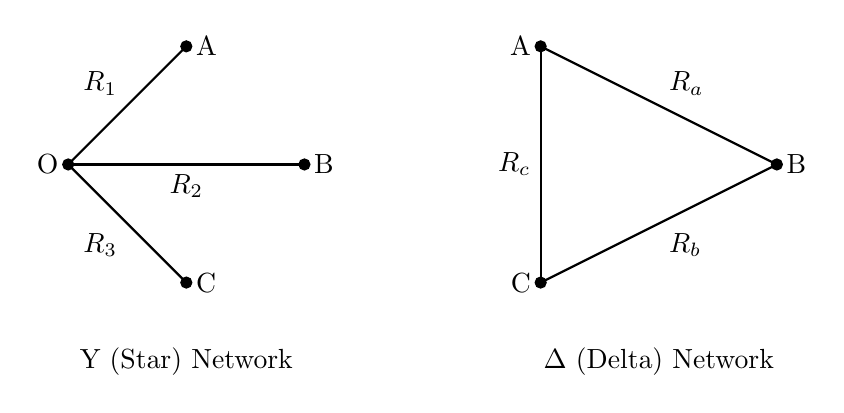
\begin{tikzpicture}
    
    % Y-configuration (Star Network)
    \draw[thick] (0,0) -- (1.5,1.5) node[midway, above left] {$R_1$};
    \draw[thick] (0,0) -- (3,0) node[midway, below] {$R_2$};
    \draw[thick] (0,0) -- (1.5,-1.5) node[midway, below left] {$R_3$};
    \draw[fill=black] (0,0) circle (2pt) node[left] {O};
    \draw[fill=black] (1.5,1.5) circle (2pt) node[right] {A};
    \draw[fill=black] (3,0) circle (2pt) node[right] {B};
    \draw[fill=black] (1.5,-1.5) circle (2pt) node[right] {C};
    \node at (1.5,-2.5) {Y (Star) Network};
    
    % Delta-configuration (Delta Network)
    \draw[thick] (6,1.5) -- (9,0) node[midway, above right] {$R_a$};
    \draw[thick] (9,0) -- (6,-1.5) node[midway, below right] {$R_b$};
    \draw[thick] (6,-1.5) -- (6,1.5) node[midway, left] {$R_c$};
    \draw[fill=black] (6,1.5) circle (2pt) node[left] {A};
    \draw[fill=black] (9,0) circle (2pt) node[right] {B};
    \draw[fill=black] (6,-1.5) circle (2pt) node[left] {C};
    \node at (7.5,-2.5) {\(\Delta \)  (Delta) Network};
    
    \end{tikzpicture}
\end{center}
    

Equating the equivalent resistance between the two networks we have 

\begin{equation}
    \begin{cases}
        R_{AB} &= R_1 +R_2 = (R_{a}^{-1} + (R_{b} + R_{c}  )^{-1}  )^{-1} ,\\
        R_{BC} &= R_2 +R_3 = (R_{b}^{-1} + (R_{a} + R_{c}  )^{-1}  )^{-1} ,\\
        R_{AC} &= R_1 +R_3 = (R_{c}^{-1} + (R_{a} + R_{b}  )^{-1}  )^{-1} . 
    \end{cases}
\end{equation}

Solving gives the transformation

\begin{center}
    \renewcommand{\arraystretch}{1.5} % Adjust row height
    \setlength{\tabcolsep}{12pt} % Adjust column width
    \begin{tabular}{|c|c|}
    \hline
    \textbf{Y to \(\Delta\) Transformation} & \textbf{\(\Delta\) to Y Transformation} \\
    \hline
    $R_a = R_2 R_3 (1/R_1 + 1/R_2 + 1/R_3 )$ & $R_1 = R_{b}R_{c}/(R_{a} + R_{b} + R_{c})  $ \\
    $R_b = R_1 R_3 (1/R_1 + 1/R_2 + 1/R_3 )$ & $R_2 = R_{a}R_{c}/(R_{a} + R_{b} + R_{c})$ \\
    $R_c = R_1 R_2 (1/R_1 + 1/R_2 + 1/R_3 )$ & $R_3 = R_{a}R_{b}/(R_{a} + R_{b} + R_{c})$ \\
    \hline
    \end{tabular}
\end{center}

\example{Equivalent Resistance (1).}
{Find the equivalent resistance of the resistor network shown in \cref{equiv1}.}
{Using the \(\Delta -Y\) transformation we can redraw the circuit as in \cref{equiv2}, then the equivalent resistance is readily calculated as \(R_{\text{eqv} } = 9R/5 \). 

Alternatively, one can simply use symmetry argument to recast the circuit as in \cref{equiv3}, which gives the same answer \(R_{\text{eqv} } = 9R/5 \). } 

\threefig{equiv1}{width=\textwidth}{equiv2}{width=\textwidth}{equiv3}{width=\textwidth}{equiv} 

\section{Superconductor}

A superconductor, in most cases can be well modelled by a perfect conductor, that is \(\sigma \rightarrow \infty\). And the most important fact about a superconductor (or a perfect conductor) is that the magnetic flux through the conductor is always constant. This is because if there is a change of magnetic flux, thus an induced emf, the current could get arbitraily large for infinitisimal small emf. In practice, when a magnetic field line try to penetrate through the conductor, a slight emf is induced which is enough to produce an induced current that generate an opposing magnetic field.

If we have a sheet of perfect conductor and put a magnet next to it, currents called ``eddy currents'' appear in the sheet so that no magnetic flux enters. The field lines in this case would look like this:

\onefig{superconductorfieldline}{scale=0.3} 

Since the currents in the magnet and the eddy currents are in opposite directions, they repel and the magnet get levitated above the sheet. If the conductor is not perfect there will be some resistance to the flow of the eddy currents. The currents will tend to die out and the magnet will slowly settle down and the flux of the magnetic field from the magnet would gradually penetrate the conductor.

Eddy currents are best illustrated by the ``pendulum'' set up shown in \cref{eddypen1}.

\twofig{eddypen1}{width=\textwidth}{eddypen2}{width=\textwidth}{eddypen} 

As the metal plate enters the gap of the magnet, there will be eddy current induced in the plate which acts to oppose the change in flux through the plate, so the current s at first bring the plate almost to a dead stop as it starts to enter the field. Then as the currents die down the plate slowly settles to rest at the equilibrium position. The nature of the eddy currents is shown in \cref{eddypen2}.  

If, for instance the copper plate is replace by one which has several narrow slots cut in it, the eddy current effects are drastically reduced, since the currents in each section of the loop have less flux to drive them so the effects of the resistance of each loop are greater. 

\example{Eddy Current.}
{Consider a spherical shell with conductivity \(\sigma \) with inner and outer radius \(R_1 \text { and } R_2 \) respectively spinning with constant angular velocity \(\boldsymbol{\omega } =  \omega \vu{x} \) under an uniform magnetic field \(\vb{B} = B \vu{z} \). Find the eddy currents in the steady state.  }
{Firstly from the continuity equation we have

\begin{equation}
    \div{\vb{J} } = \sigma \left( \div{\vb{E} } + \div{(\vb{v} \cross \vb{B} )}   \right) = \sigma \left( \frac{\rho }{\epsilon_0 } + \div{(\vb{v} \cross \vb{B} )}   \right) = -\frac{\partial \rho }{\partial t} = 0.
\end{equation}

So the charge density \(\rho \) is given by 

\begin{equation}
    \begin{aligned}
    \rho &= -\epsilon_0 \div{(\vb{v} \cross \vb{B} )} = -\epsilon_0 \div{((\boldsymbol{\omega } \cross \vb{r} )\cross \vb{B} )} \\ 
    &= -\epsilon_0 \div{(\vb{r} (\vb{B} \cdot \boldsymbol{\omega } ) - \boldsymbol{\omega }(\vb{B} \cdot \vb{r} ) )} =  - \epsilon_0 \div{(-\omega By \vu{x} )} = 0. 
    \end{aligned}
\end{equation}

The Laplace's equation \(\laplacian V = 0\) thus holds within the shell, with the boundary conditions

\begin{equation}
    J_{r} = \sigma (\vb{E} +\vb{v} \cross \vb{B} ) \cdot \vu{r} = 0 \text{ at } r=  R_1 \text { and } R_2 .  
\end{equation}

In terms of potential, 

\begin{equation}
    E_{r} = -\frac{\partial V}{\partial r} = -(\vb{v} \cross \vb{B} ) \cdot \vu{r} = \omega By(\vu{x} \cdot \vu{r} )= \begin{cases}
        \omega BR_1 \sin ^2\theta \sin \phi \cos \phi  &\text{ at } r = R_1 ,\\
        \omega BR_2 \sin ^2\theta \sin \phi \cos \phi  &\text{ at } r = R_2 .
    \end{cases} 
\end{equation}

The potential is thereofore unqiuely determined and can be easily guessed as 

\begin{equation}
    V(r, \theta ,\phi ) = -\frac{1}{2}\omega Br^2\sin ^2\theta \sin \phi \cos \phi ,  
\end{equation}

and the eddy current can be found by 

\begin{equation}
    \vb{J} = \sigma (\vb{E} + (\vb{v} \cross \vb{B} )) =  -\sigma \grad{V} = \frac{1}{2} \omega B\sigma r\sin \theta \vu{\boldsymbol{\phi } } . 
\end{equation}

One can prove that for \(\omega \text { and }  \vb{B} \) at arbitrary orientations the formula is 

\begin{equation}
    \vb{J} = - \frac{\sigma }{2} (\vb{r} \cross (\boldsymbol{\omega } \cross \vb{B}  )). 
\end{equation}

In particular, when \(\boldsymbol{\omega } \parallelsum \vb{B}  \), \(\vb{J} =0\) since the electric force exactly cancels the magnetic force.

Note that \(\sigma \) has to be sufficiently small or else we would need to take into account the magntic field produced by the eddy current, appearing as the self-inductance term, which lowers the electric field thus the induced eddy current. Also high \(\sigma \) implies low skin depth, so the magnetic field may not penetrate fully into the shell. 
} 


\section{Operational Amplifiers}

The shematic diagram of an operational amplifier is shown below

\begin{center}
    \begin{circuitikz}
        % Draw the op-amp triangle
        \draw (0,0) node[op amp, noinv input up] (opamp) {};
        
        % Inputs with circles at the ends
        \draw (opamp.-) -- ++(-0.5,0)             node[ocirc, inner sep=1.5pt] {}  node[left] {$V_\text{in}^-$};
        \draw (opamp.+) -- ++(-0.5,0)             node[ocirc, inner sep=1.5pt] {}  node[left] {$V_\text{in}^+$};
        
        % Output with circle at the end
        \draw (opamp.out) -- ++(0.5,0)             node[ocirc, inner sep=1.5pt] {}  node[right] {$V_\text{out}$};
        
        % Power supplies with circles at the ends
        \draw (opamp.up) -- ++(0,0.5)             node[ocirc, inner sep=1.5pt] {}  node[above] {$V_\text{cc}^+$};
        \draw (opamp.down) -- ++(0,-0.5)             node[ocirc, inner sep=1.5pt] {}  node[below] {$V_\text{cc}^-$};
    \end{circuitikz}
\end{center}

In the diagram, \(V_{\text{cc} }^{\pm }  \) are the power supply voltages, which are usually omitted. \(V_{\text{in} }^{\pm }  \) are the input voltages and \(V_{\text{out} } \) is the output voltage.   

The characteristic equation of an op-amp is 

\begin{equation}
    V_{\text{out} } = A_{\text{OL}} (V_{\text{in} }^+ - V_{in}^- )  
\end{equation}

Typically, the open-loop voltage gain \(A_{\text{OL}}\) is very large \((\sim 10^{5} )\) , but the output voltage \(V_{\text{out}}\) is limited within a range set by two saturation voltages \(V_{\text{sat}}^{\pm} \approx V_{\text{cc}}^{\pm} \mp 1V\). This implies that any small difference between the op-amp inputs will cause the output to saturate.

\subsection{Non-Linear Applications}
An op-amp can be used as a comparator: 


\begin{center}
    \begin{circuitikz}
        % Draw the op-amp triangle
        \draw (0,0) node[op amp, noinv input up] (opamp) {};
        
        % Non-inverting input (Vin+)
        \draw (opamp.+) -- ++(-0.5,0) 
            node[ocirc, inner sep=1.5pt] {} 
            node[left] {$V_\text{in}$};
        
        % Inverting input connected to a battery
        \draw (opamp.-) -- ++(-0.5,0) 
            to[battery, l_=1V] ++(0,-1.5)
            node[ground] {};

        % Output (Vout)
        \draw (opamp.out) -- ++(0.5,0) 
            node[ocirc, inner sep=1.5pt] {} 
            node[right] {$V_\text{out}$};
    \end{circuitikz}
\end{center}

If the inverting input signal is fixed at, say \(1V\), then the output voltage will be positive if the input signal is greater than \(1V\), and negative if the input signal is smaller than \(1V\). Since the saturation voltages are reached pratically instantly, we would get a square wave on the output signal in response to some arbitrary input signal wandering around the level of the fixed voltage at the inverting input, as shown in \cref{comparator}. 

\onefig{comparator}{scale=0.3} 

\subsection{Input and Output Impedance}

\subsubsection{Input impedance}
The input impedance \(Z_{\mathrm{in}}\) is the impedance “seen” by whatever is driving the input of a circuit or device.  Formally, if you attach a test source \(V_{\mathrm{test}}\) to the input terminals (with all other internal sources turned off) and measure the resulting current \(I_{\mathrm{test}}\) drawn into the device, then
\[
Z_{\mathrm{in}}
\;=\;
\frac{V_{\mathrm{test}}}{I_{\mathrm{test}}}.
\]
A high \(Z_{\mathrm{in}}\) means the device hardly loads the source feeding it.

\subsubsection{Output impedance}
The output impedance \(Z_{\mathrm{out}}\) is the impedance “seen” by a load attached to the output of a circuit or device.  You determine it by “looking back” into the output terminals: turn off all independent internal sources (voltage sources \(\to\) short; current sources \(\to\) open), apply a test source \(V_{\mathrm{test}}\) at the output, measure the resulting test current \(I_{\mathrm{test}}\), and compute
\[
Z_{\mathrm{out}}
\;=\;
\frac{V_{\mathrm{test}}}{I_{\mathrm{test}}}.
\]
A low \(Z_{\mathrm{out}}\) means the device can drive heavy loads without its output voltage dropping.

\subsubsection{Why they matter}
\begin{itemize}
  \item A high \(Z_{\mathrm{in}}\) ensures minimal signal loss: the preceding stage “sees” almost no load.
  \item A low \(Z_{\mathrm{out}}\) ensures good voltage regulation: the following stage receives nearly the full intended output voltage, even if it draws significant current.
\end{itemize}

Any circuit device can be treated as a black box with four terminals, two for the inputs and two for the outputs. For the two input terminals, the device act as a resistor, so you can determine the input resistance \(Z\) by measuring the current \(I\) when you connect the terminal with a voltage source with a voltage source \(V\), with \(Z = V/I\). For the two output terminals, the device acts as a voltage source connected to its internal resistance, so the output impedance \(Z\) can be determine by connecting the terminals with a variable resistor and varies its resistance from \(0 \to R\) which the voltage reduce from \(V \to V/2\).   

\subsection{Linear Applications}

We can state the three ``golden rules'' of an ideal linear op-amp:

\begin{enumerate}
    \item The output will do whatever is necessary to make the voltage difference between the inputs zero because the loop gain is infinity.\footnote{Note that it does not mean that the op-amp acutally changes the voltage at the inputs. What it does is ``look'' at its input terminals and swing its output terminal around so that the external feedback betwork brings the input differential to zero.}
    \item No current flows into the inputs becuase the input impedance is infinity (but current can flow out of the output).
    \item The output voltage is independent of the output current since the output impedance is zero.
\end{enumerate}

Input impedance is the ipedance ``seen'' by whatever is driving the input of a device. Formally if you attach a test source \(V_{\text{test} } \) to the input terminals and measure the resulting current \(I_{\text{test} } \) drawn into the device then 

\begin{equation}
    Z_{\text{in} } = \frac{V_{\text{test} } }{I_{\text{test} } }.
\end{equation}

Output impedance is the impedance ``seen'' by a load attached to the output of a device. 

For example, the input resistance is the resistance between the driving-point voltage and point \(A\), \textit{i.e.,} \(R_1 \). The output resistance is the resistance between the output voltage and the output of the op-amp, \textit{i.e.,} 0.

\subsubsection{Simple Inverting Amplifier}

A simple inverting amplifier is shown in \cref{invertingopamp}.

\onefig{invertingopamp}{scale=0.3} 

Since \(B\) is at ground, so by the first ``golden rules'' \(A\) is also at ground. Therefore the voltage across \(R_2 \) is \(V_{\text{out}} \) and the voltage across \(R_1 \) is \(V_{\text{in}} \). And by the second ``golden rules'' we have \(V_{\text{out} } /R_2 = - V_{\text{in} }/ R_1  \). 

Note that the positive terminal of the op-amp is grounded but not the negative terminal. This is crucial for the feedback loop to work properly. In a non-inverting amplifier the ground and the input voltage is swapped.

To understand what is really happening, imagine initially all the terminals are at zero voltage, now \(V_{\text{in}} \) is raised to \(+1V\). Due to the enormous input unbalance, \(V_{\text{out}} \) is dropped to the saturation voltage.

When the output terminal is connected to a load of reisistance \(R_{\text{load} } \), then the power gain would be 

\begin{equation}
    P = \frac{V_{\text{in} }^2 /R_{1 }  }{V_{\text{out} }^2/ R_{\text{load} }  } = \frac{R_{1} }{R_{\text{load} } } \frac{R_{1}^2 }{R_{2}^2 }.  
\end{equation}

\subsubsection{Summing and Difference Amplifier}

A summing amplifier and a difference amplifier are shown in \cref{sumdifamp}.

For the summing amplifier from the figure we have 

\begin{equation}
    i = \frac{V_1 }{R_1 } + \frac{V_2 }{R_1 } + \frac{V_3 }{R_1 } = -\frac{V_{\text{out} } }{R_2 } \implies V_{\text{out} } = -\frac{R_2 }{R_1 } (V_1 +V_2 +V_3 ).    
\end{equation}

For the difference amplifier from the figure we have 

\begin{equation}
    V_{+} = \frac{R_2 }{R_1 +R_2 }V_2 = V_{-} = \frac{R_2 V_1 +R_1 V_{\text{out} } }{R_1 +R_2 } \implies V_{\text{out} } = \frac{R_2 }{R_1 }(V_2 -V_1 ).     
\end{equation}

\twofig{sumamp}{width=\textwidth}{difamp}{width=\textwidth}{sumdifamp} 

\subsubsection{Differentiator and Integrator}

A differentiator and an integrator are shown in \cref{diffintamp}.

For the differentiator from the figure we have

\begin{equation}
    V_{\text{out} } = -iR = -RC \frac{dV_{\text{in} } }{dt}. 
\end{equation}

For the integrator from the figure we have

\begin{equation}
    V_{\text{out} } = -\frac{1}{C} \int_{0}^{t} idt = -\frac{1}{RC} \int_{0}^{t} V_{\text{in} }dt.    
\end{equation}

\twofig{diffamp}{width=\textwidth}{intamp}{width=\textwidth}{diffintamp} 

Note that if the input voltage has any DC offset the integral would diverge. To prevent that put a large resistor \(R_{f} \) in parallel with the capacitor \(C\), so when \(\omega = 0\) we have a finite offset. 



\subsubsection{High Pass Filter}

A high pass filter is shown in \cref{highpassfilter}.

From the figure we have 

\begin{equation}
    V_{\text{out} } = -iR_2 = -\frac{V_0 e^{j \omega t} }{R_1 -j /\omega C} = -\frac{j \omega C R_2 e^{j \omega t} }{1+j \omega CR_1 } V_0.  
\end{equation}

As \(\omega \to 0\), \(V_{\text{out} } \to 0\) and as \(\omega \to \infty\), \(V_{\text{out} } \to -(R_2 /R_1 )V_0 e^{j \omega t} \).    

Its advantages compared to a dc version of a high pass filter is that the gain can be controlled by the ratio of the resistor, and the load (impedance between \(V_{\text{out} } \) and ground) does not affect the transfer function. However its input impedance is finite, so it would not take all of the voltage's source voltage since the voltage source might have internal impedance.

\onefig{highpassfilter}{scale=0.3} 

\example{Digital to Analogue Converter.}
{Refer to \cref{dac}, find \(V_{\text{out} } \) in terms of \(V_{\text{in} }\text { and } R \).  }
{Since the inverting input is virtually grounded, so the potential at the position of the switch is always zero regardless of the state of the switch, and can be combined with the true ground at the upper right corner of the diagram.

The swtich simply determine whether the current flowing through each bracnhes flows towards the op-amp, or into the ground. Combining the resistors using simple techniques, the voltages at the top of the resistors at each branches are \(V_{\text{in} }, V_{\text{in} } /2, V_{\text{in} } /4  \text { and } V_{\text{in} }/8  \) respectively. 

Thus the total current flowing towards the op-amp is

\begin{equation}
    I = I_0 + I_1 + I_2 + I_3 = \frac{V_{\text{in} } }{2R}\left( S_0 + \frac{S_1}{2} + \frac{S_2 }{4} + \frac{S_3}{8} \right). 
\end{equation}

The output voltage is thus 

\begin{equation}
    V_{\text{out} } = - IR =  - \frac{V_{\text{in} } }{2}\left( S_0 + \frac{S_1}{2} + \frac{S_2 }{4} + \frac{S_3}{8} \right),
\end{equation}

where \(S_{i} = 1\) if the \(i^{\text{th}} \) switch is closed, and 0 otherwise.   
} 

\onefig{dac}{scale=0.5} 


\chapter{Conservation Laws}

\section{Charge Conservation}

The local conservation of charge tells us that if the charge in some region changes, then exactly that amount of charge must have passed in or out through the surface, so 

\begin{equation}
    \frac{dQ}{dt} = \int_{V}^{} \frac{\partial \rho }{\partial t} d\tau =   -\oint_{S} \vb{J} \cdot d\vb{S}  = -\int_{V}^{} (\grad{\vb{J} } ) d\tau   \implies \frac{\partial \rho }{\partial t} = - \div{\vb{J} }.   \label{contincharge} 
\end{equation}

Note that this continuity equation is not an independent assumption but can be derived from the Maxwell's equations.

\section{Energy Conservation}

Suppose we have some charge and current configuration which, at time \(t\) produces fields \(\vb{E} \text { and } \vb{B} \). In the next instant, \(dt\), the charges move around a bit. The work done, \(dW\), by the electromagnetic forces on a charge \(q\), is then 

\begin{equation}
    dW = q(\vb{E} + \vb{v} \cross \vb{B} ) \cdot (\vb{v} dt) \implies \frac{dW}{dt} = \int_{V}^{} (\vb{E} \cdot \vb{J} )d\tau . \label{dW} 
\end{equation}

From the Ampere's law (\cref{comampere}), we have 

\begin{equation}
    \begin{aligned}
        \vb{E} \cdot \vb{J} &= \frac{1}{\mu_0 } \vb{E} \cdot (\curl{\vb{B} } ) - \epsilon_0 \vb{E} \cdot \frac{\partial \vb{E} }{\partial t} \\
        &= \frac{1}{\mu_0 } \left( \vb{B} \cdot (\curl{\vb{E} } ) - \div{(\vb{E} \cross \vb{B} )}  \right) - \frac{\epsilon_0 }{2} \frac{\partial E^2}{\partial t} \\
        &= \frac{1}{\mu_0 } \left( -\vb{B} \cdot \frac{\partial \vb{B} }{\partial t} - \div{(\vb{E} \cross \vb{B} )}   \right) - \frac{\epsilon_0 }{2} \frac{\partial E^2}{\partial t}\\
        &= -\frac{1}{2} \frac{\partial }{\partial t} \left( \epsilon_0 E^2 + \frac{1}{\mu_0 } B^2  \right)  - \frac{1}{\mu_0 } \div{(\vb{E} \cross \vb{B} )}.         
    \end{aligned}
\end{equation}

So plugging this for the \(\vb{E} \cdot \vb{J} \) in \cref{dW}, we have

\begin{equation}
    \begin{aligned} 
    \frac{dW}{dt} &=  \int_{V}^{}\left( -\frac{1}{2} \frac{\partial }{\partial t} \left( \epsilon_0 E^2 + \frac{1}{\mu_0 } B^2  \right)  - \frac{1}{\mu_0 } \div{(\vb{E} \cross \vb{B} )} \right) d\tau \\
    &= -\frac{d}{dt} \int_{V}^{} \frac{1}{2} \left( \epsilon_0 E^2 + \frac{1}{\mu_0 }B^2  \right) d\tau - \frac{1}{\mu_0 } \oint_{S} (\vb{E} \cross \vb{B} ) \cdot d\vb{S'} \footnote{We used \(\vb{S} '\) to denote the vector area to avoid confusion with the Poynting vector \(\vb{S} \).} \\
    &\equiv -\frac{d}{dt} \int_{V}^{} ud\tau - \oint_{S} \vb{S} \cdot d\vb{S'}.
    \end{aligned} 
\end{equation}

Here the total energy stored in electromagnetic fields, per unit volume, is 

\begin{equation}
    u \equiv  \frac{1}{2} \left( \epsilon_0 E^2 + \frac{1}{\mu_0 } B^2  \right),
\end{equation}

whil the energy per unit time, per unti area, transported by the fiels, called the Poynting vector, is

\begin{equation}
    \vb{S} \equiv \frac{1}{\mu_0 } \left( \vb{E} \cross \vb{B}  \right)  = \vb{E} \cross \vb{H} .
\end{equation}

The Poynting's theorem then states that the decrease in energy stored by the electromagnetic fields in a certain volume (the first term on the RHS) is equals to the work done on the charges by the electromagnetic force (the term on the left), plus the energy that flows out through the surface (the second term on the right).

If there is no work done on the charges, \textit{i.e.,} \(dW /dt = 0\), then

\begin{equation}
    \int_{V}^{} \frac{\partial u}{\partial t} d\tau = -\oint_{S} \vb{S} \cdot d\vb{S'} = -\int_{V}^{} (\div{\vb{S} } ) d\tau  \implies \frac{\partial u}{\partial t} = -\div{\vb{S} },   \label{continenergy} 
\end{equation}

which is exactly analogous to the charge continuity equation (\cref{contincharge}), where the energy density \(u\) plays the role of the charge density \(\rho \) and the Poynting vector (energy current density) \(\vb{S} \) plays the role of the current density \(\vb{J} \). 

\section{Momentum Conservation}

\subsection{Maxwell's Stress Tensor}

The Maxwell's Stress Tensor \(\boldsymbol{\sigma } \) is defined as 

\begin{equation}
    \sigma _{ij}  = \epsilon_0 \left( E_{i}E_{j} - \frac{1}{2} \delta _{ij} E^2     \right) + \frac{1}{\mu_0 }\left( B_{i}B_{j} - \frac{1}{2} \delta _{ij}B^2     \right),
\end{equation}

which is the force per unit area in the \(i^{\text{th}} \) direction acting on an element of surface oriented in the \(j^{\text{th}} \) diretion. Diagonal elements \((\sigma _{ii}, \sigma _{jj}, \sigma _{kk}  )\) represents pressure and ``off-diagonal'' elements are shears.

The divergence of \(\boldsymbol{\sigma }  \) is then 

\begin{equation}
    \begin{aligned}
        (\div{\boldsymbol{\sigma }  } )_{j} =  \partial _{i}\sigma _{ij} = \epsilon_0 \left( (\div{\vb{E} } )E_{j} + (\vb{E} \cdot \grad{} )E_{j} - \frac{1}{2}\grad{}_{j}E^2      \right) + \frac{1}{\mu_0 } \left( (\div{\vb{B} } )B_{j}+(\vb{B} \cdot \grad{} )B_{j}-\frac{1}{2}\grad{}_{j}B^2      \right).   
    \end{aligned}
\end{equation}

\example{Forces between Hemispheres of a Sphere.}
{Here we revisit an example in \cref{surcha} and calculate the net force between the hemispheres of a sphere with radius \(R\) and charge \(Q\).}
{Since the system is static and symmetic along the \(z\)-axis, the force is 

\begin{equation}
    F = \oint_{S} (\boldsymbol{\sigma } \cdot d\vb{S}  )_{z}.
\end{equation}

For the hemispherical bowl, the infinitesimal vector area is 

\begin{equation}
    d\vb{S} = R^2\sin \theta d \theta d\phi \vu{r} = R^2\sin \theta d \theta d\phi (\sin \theta \cos \phi \vu{x} + \sin \theta \sin \phi \vu{y} + \cos \theta \vu{z} ),
\end{equation}

and the electric field is 

\begin{equation}
    \vb{E} = \frac{1}{4\pi \epsilon_0} \frac{Q}{R^2}\vu{r} = \frac{1}{4\pi \epsilon_0} \frac{Q}{R^2} (\sin \theta \cos \phi \vu{x} + \sin \theta \sin \phi \vu{y} +\cos \theta \vu{z}),
\end{equation}

so the relevant components of the Maxwell's stress tensor are 

\begin{equation}
    \begin{aligned}
        \sigma _{zx} &= \epsilon_0 E_{z}E_{x} = \epsilon_0 \left( \frac{Q}{4\pi \epsilon_0 R^2}  \right)^2 \sin \theta \cos \theta \cos \phi \\
        \sigma _{zy} &= \epsilon_0 E_{z}E_{y} = \epsilon_0 \left( \frac{Q}{4\pi \epsilon_0 R^2}  \right)^2 \sin \theta \cos \theta \sin \phi \\
        \sigma _{zz} &= \frac{\epsilon_0 }{2}\left( E_{z}^2- E_{x}^2-E_{y}^2    \right) = \frac{\epsilon_0 }{2} \left( \frac{Q}{4\pi \epsilon_0 R^2}   \right)^2 (\cos ^2\theta - \sin ^2\theta ),
    \end{aligned}
\end{equation}

and the integrand is therefore

\begin{equation}
    (\boldsymbol{\sigma } \cdot d\vb{S} )_{z} =  \sigma _{zx}dS_{x} + \sigma _{zy}dS_{y}+ \sigma _{zz}dS_{z} = \frac{\epsilon_0 }{2} \left( \frac{Q}{4\pi \epsilon_0 R}   \right)^2 \sin \theta \cos \theta d \theta d\phi .       
\end{equation}

For the circular disk, the infinitesimal vector area is 

\begin{equation}
    d\vb{S} = -r dr d\phi \vu{z} ,
\end{equation}

and the electric field is 

\begin{equation}
    \vb{E} = \frac{1}{4\pi \epsilon_0} \frac{Q}{R^3 }\vb{r} = \frac{1}{4\pi \epsilon_0} \frac{Qr}{R^3 }(\cos \phi \vu{x} + \sin \phi \vu{y} ).  
\end{equation}

so the relevant component of the Maxwell's stress tensor is 

\begin{equation}
    \sigma _{zz} = \frac{\epsilon_0 }{2}\left( E_{z}^2 - E_{x}^2 - E_{y}^2    \right) = - \frac{\epsilon_0 }{2} \left( \frac{Q}{4\pi \epsilon_0 R^3 }  \right)^2r^2,
\end{equation}

and the integrand is therefore

\begin{equation}
    (\boldsymbol{\sigma } \cdot d\vb{S}  )_{z} =  \sigma _{zz}dS_{z} = \frac{\epsilon_0 }{2} \left( \frac{Q}{4\pi \epsilon_0 R^3 }  \right)^2 r^3 dr d\phi .  
\end{equation}

The total force is finally 

\begin{equation}
    F = \frac{\epsilon_0 }{2} \left( \frac{Q}{4\pi \epsilon_0 R}  \right)^2 2\pi \int_{0}^{\frac{\pi }{2} } \sin \theta \cos \theta d \theta + \frac{\epsilon_0 }{2} \left( \frac{Q}{4\pi \epsilon_0 R^3 }  \right)^2 2\pi \int_{0}^{R} r^3 dr = \frac{1}{4\pi \epsilon_0} \frac{3Q^2}{16R^2}
\end{equation}

as expected.

In fact, any volume that encloses all of the charge in question (and no other charge) will do the job. For example, we can use the whoele region \(z > 0\). In place of the hemispherical bowl, we now have the outer portion of the plane, so the only relevant component of the Maxwell's stress tensor can be found by substituting \(\theta = \pi /2\) into the \(\sigma _{zz} \) found above as

\begin{equation}
    \sigma _{zz} = - \frac{\epsilon_0 }{2} \left( \frac{Q}{4\pi \epsilon_0 }  \right)^2 \frac{1}{r^4},    
\end{equation} 

so the integrand is 

\begin{equation}
    (\boldsymbol{\sigma }\cdot d\vb{S}  )_{z} = \frac{\epsilon_0 }{2} \left( \frac{Q}{4\pi \epsilon_0 }  \right)^2 \frac{1}{r^3 }dr d\phi ,   
\end{equation}

and the force is 

\begin{equation}
    F = \frac{\epsilon_0 }{2} \left( \frac{Q}{4\pi \epsilon_0 }  \right)^2 2\pi \int_{R}^{\infty} \frac{1}{r^3 }dr = \frac{1}{4\pi \epsilon_0} \frac{Q^2}{8R^2}.     
\end{equation}
}


\example{Pinch Pressure.}
{Find the pressure experienced by the wall when a current \(I\) flows in a long cylinder of radius \(R\).}
{} 


\subsection{Momentum Continuity Equation}

To derive a continuity equation for momentum, we start by finding the totoal force \(\vb{F} = d\vb{p} /dt\) acting on a charge \(q\) in the same setting as in the previous section. 

\begin{equation}
    \vb{F} = \frac{d\vb{p} }{dt}  = q(\vb{E} + \vb{v} \cross \vb{B} ) = \int_{V}^{} (\rho \vb{E} + \vb{J} \cross \vb{B}) d\tau . 
\end{equation}

As usual, we will eliminate \(\rho \text { and } \vb{J} \) using the Gauss's law and the Ampere's law (\cref{gauss, comampere}) to simplify the force per unit volume \(\vb{f} = \rho \vb{E} + \vb{J} \cross \vb{B} \) 

\begin{equation}
    \begin{aligned}
        \vb{f}  &= \epsilon_0 (\div{\vb{E} } )\vb{E}  + \left( \frac{1}{\mu_0} \curl{\vb{B} } - \epsilon_0 \frac{\partial \vb{E} }{\partial t}    \right) \cross \vb{B} \\
        &= \epsilon_0 (\div{\vb{E} } )\vb{E}  - \frac{1}{\mu_0 }\vb{B} \cross (\curl{\vb{B} } ) - \epsilon_0 \left( \frac{\partial }{\partial t} \left( \vb{E} \cross \vb{B}  \right) - \left( \vb{E} \cross \frac{\partial \vb{B} }{\partial t}  \right) \right) \\
        &= \epsilon_0 \left( (\div{\vb{E} } )\vb{E}  - \vb{E} \cross (\curl{\vb{E} } ) \right) - \frac{1}{\mu_0} \vb{B} \cross (\curl{\vb{B} } ) - \epsilon_0 \frac{\partial }{\partial t} (\vb{E} \cross \vb{B} ).
    \end{aligned}
\end{equation}

To make things look more symmetrical, we throw in a term \((\div{\vb{B} } )\vb{B} =0\), and use the identity 

\begin{equation}
    \grad{E^2} = 2\left( \vb{E} \cdot \grad{}  \right) \vb{E} +2\vb{E} \cross (\curl{\vb{E} } )
\end{equation}

to get the force density \(\vb{f} \) as 

\begin{equation}
    \begin{aligned}
       \vb{f}  &= \epsilon_0 \left( (\div{\vb{E} } )\vb{E} + (\vb{E} \cdot \grad{} )\vb{E}  \right) + \frac{1}{\mu_0 } \left( (\div{\vb{B} } )\vb{B}  + (\vb{B} \cdot \grad{} )\vb{B}  \right) \\
        &~~~~ - \frac{1}{2} \grad{\left( \epsilon_0 E^2 + \frac{1}{\mu_0 }B^2 \right)} - \epsilon_0 \frac{\partial }{\partial t} \left( \vb{E} \cross \vb{B}  \right).
        \end{aligned}
\end{equation}

So the force density \(\vb{f} \) becomes

\begin{equation}
    \vb{f} = \div{\boldsymbol{\sigma } } - \epsilon_0 \mu_0 \frac{\partial \vb{S} }{\partial t},    
\end{equation}

and the total force \(\vb{F} \) is therefore

\begin{equation}
    \begin{aligned} 
    \vb{F} = \frac{d\vb{p} }{dt} &= \oint_{S} \boldsymbol{\sigma } \cdot d\vb{S} - \epsilon_0 \mu_0 \frac{d}{dt} \int_{V}^{} \vb{S} d\tau \\
    &\equiv - \frac{d}{dt} \int_{V}^{} \vb{g}  d\tau + \oint_{S} \sigma \cdot d\vb{S} .
    \end{aligned}   
\end{equation}

Here the total momentum stored in electromagnetic fields, per unit volume, is 

\begin{equation}
    \vb{g} = \epsilon_0 \mu_0 \vb{S} = \frac{\vb{S} }{c^2} = \epsilon_0 (\vb{E} \cross \vb{B} ) = (\vb{D} \cross \vb{B} ), 
\end{equation}

while the momentum per unit time, per unit area, transported by the fields, is the (negative of) Maxwell's stress tensor \(-\boldsymbol{\sigma } \). 

The momentum conservation law then states that the decrease in momentum stored by the electromagnetic fields in a certain volume (the first term on the RHS) is equals to the impulse received by the charges by the electromagnetic force (the term on the right), plus the momentum that flows out through the surface (the second term on the right).

If there is no force on the charges, \textit{i.e.,} \(d\vb{p} /dt = 0\), then 

\begin{equation}
    \int_{V}^{} \frac{\partial \vb{g} }{\partial t} d\tau = \oint_{S} \boldsymbol{\sigma } \cdot d\vb{S} = \int_{V}^{} (\div{\boldsymbol{\sigma } } ) d\tau \implies \frac{\partial \vb{g} }{\partial t} = \div{\boldsymbol{\sigma } },  \label{continmomentum} 
\end{equation}

which is exactly analogous to the charge and energy continuity eqution \cref{contincharge, continenergy}, where the momentum density \(\vb{g} \) plays the role of the charge and energy density \(\rho \text { and } u\) and the (negative of) Maxwell's stress tensor (momentum current density) \(-\boldsymbol{\sigma } \) plays the role of the current dnesity and the Poynting's vector \(\vb{J} \text { and } \vb{S} \).     

\example{Resistancelses Coaxial Cable.}
{As shown in \cref{coax}, a resistanceless coaxial cable of length \(l\) consists of an inner and an outer conductor at \(r = a \text { and } b\) respectively. It is connected to a battery at one end and a resistor at the other. 

The inner conductor carries a unifrom charge per unit length \(\lambda \) and a steady current \(I\) to the right while the outer conductor has opposite charge and current. Find the electromagnetic momentum stored in the fields.}
{The fields are 

\begin{equation}
    \vb{E} = \frac{1}{2\pi \epsilon_0 } \frac{\lambda }{s} \vu{\boldsymbol{\rho }} ~\text { and }~ \vb{B} = \frac{\mu_0 }{2\pi } \frac{I}{s} \vu{\boldsymbol{\phi }},      
\end{equation}

so the Poynting vector is 

\begin{equation}
    \vb{S} = \frac{\lambda I}{4\pi ^2\epsilon_0 s ^2}\vu{z}. 
\end{equation}

So energy is flowing downn the line, from the battery to the resistor. In fact, the power transported is 

\begin{equation}
    \vb{P} = \int \vb{S} \cdot d\vb{S} ' = \frac{\lambda I}{4\pi ^2\epsilon_0 } \int_{a}^{b} \frac{1}{s ^2} 2\pi s ds= \frac{\lambda I}{2\pi \epsilon_0 } \ln \left( \frac{b}{a}  \right) = IV, 
\end{equation}

as it should be..

The momentum in the fields is 

\begin{equation}
    \vb{p} = \mu_0 \epsilon_0 \int \vb{S} d\tau = \frac{\mu_0 \lambda I}{4\pi ^2}\vu{z} \int_{a}^{b} \frac{1}{s ^2}2\pi s lds = \frac{\mu_0 \lambda Il}{2\pi } \ln \left( \frac{b}{a}  \right) \vu{z} = \epsilon_0 \mu_0 IVl \vu{z} .    
\end{equation}

Suppose now that we turn up the resistance, so the current decreases. The changing magnetic field will induce an electric field, which can be found by considering a rectangular loop in the coaxial cable as

\begin{equation}
    \oint_{C} \vb{E} \cdot dl = E(\rho _{0} )l - E(\rho )l = -\frac{d}{dt} \int \vb{B} \cdot d\vb{S} = - \frac{\mu_0 l}{2\pi } \frac{dI}{dt} (\ln \rho  - \ln \rho _0 ), 
\end{equation}

so the electric field is 

\begin{equation}
    \vb{E} (\rho ) = \left( \frac{\mu_0 }{2\pi } \frac{dI}{dt} \ln \rho +K  \right) \vu{z}.
\end{equation}

The momentum imparted to the cable as the current drops from \(I\) to 0, is therefore

\begin{equation}
    \begin{aligned} 
    \vb{p}_{\text{mech} }  &= \int \vb{F} dt = \int \left(\lambda l \left( \frac{\mu_0 }{2\pi } \frac{dI}{dt} \ln a + K  \right)\vu{z} - \lambda l \left( \frac{\mu_0 }{2\pi } \frac{dI}{dt} \ln a + K  \right)\vu{z}\right) dt \\ 
    &= \frac{\mu_0 \lambda Il}{2\pi } \ln \left( \frac{b}{a}  \right)\vu{z} = \vb{p} .
    \end{aligned} 
\end{equation}

} 

\onefig{coax}{scale=0.3} 


\section{Angular Momentum Conservation}

The angular momentum density is simply 

\begin{equation}
    \vb{l} = \vb{r} \cross \vb{g} = \epsilon_0 (\vb{r} \cross (\vb{E} \cross \vb{B} )).
\end{equation}

\chapter{Electromagnetic Waves}

\section{Reflection and Transmission}

For a plane electromagnetic wave \(\vb{E} (\vb{r} ,t) = \vb{E} _{0}(r)e^{i (\vb{k} \cdot \vb{r} -\omega t)} \text { and } \vb{B} (\vb{r} ,t) = \vb{B} _{0}e^{i(\vb{k} \cdot \vb{r} -\omega t)}\),\footnote{Rigorously, the electric field is \(\vb{E} (\vb{r} ,t) = \mathfrak{Re} (\vb{E} _{0}(\vb{r} ) e^{i(\vb{k} \cdot \vb{r} -\omega t)}  ) \), but in most cases we can simply omit the \(\mathfrak{Re} \) operator since the actual complex wave also satisfiy the Maxwell's equations due to their linearity. One can add its complex conjugate \(\vb{E} _{0}^* e^{-i(\vb{k} \cdot \vb{r} -\omega t)}  \) to make it real, but then the new amplitude is half the previous one and it is an unnecessary complication. As long as we take the real part at the end this two expressions are equivalent. The same holds for the magnetic field.} we have from Faraday's law that 

\begin{equation}
    i \vb{k} \cross \vb{E} _{0} = - i\omega \vb{B} _{0} \implies   \vb{B} _{0} = \frac{\vb{k} \cross \vb{E} _{0} }{\omega }  
\end{equation}

Refer to \cref{oblique}, where the incidence monochromatic plane wave has a polarization (electric field direction) parallel to the plane of incidence\footnote{A general polarization can be thought of the linear combination of the parallel and the perpendicular polarization.} 

\onefig{oblique}{scale=0.3} 

\begin{equation}
    \vb{E} _{I}  = \vb{E} _{0,I} e^{i(\vb{k} _{I}\cdot \vb{r} -\omega t )}, \quad \vb{B} _{I} = \frac{\vb{k}_{R}  \cross \vb{E} _{0,R} }{\omega } e^{i(\vb{k} _{I}\cdot \vb{r} -\omega t )}.     
\end{equation}

gives rise to a reflected wave 

\begin{equation}
    \vb{E} _{R} = \vb{E} _{0,R} e^{i(\vb{k} _{R} \cdot \vb{r} - \omega t )}, \quad \vb{B} _{R} = \frac{\vb{k} _{R} \cross \vb{E} _{0,R}  }{\omega }   
\end{equation}

and a transmitted wave

\begin{equation}
    \vb{E} _{T} = \vb{E} _{0,T} e^{i(\vb{k} _{T} \cdot \vb{r} -\omega t )}, \quad \vb{B} _{T} = \frac{\vb{k} _{T} \cross \vb{E} _{0,T}  }{\omega }.   
\end{equation}

The boundary conditions are given by \cref{boundary}. Here we assume that the free charge density \(\rho _{f} \) and the free current density \(\vb{J} _{f} \) are zero.   

All of them share the generic structure 

\begin{equation}
    ()e^{i(\vb{k} _{I}\cdot \vb{r} -\omega t )} + ()e^{i(\vb{k} _{R}\cdot \vb{r} - \omega t)} = () e^{i(\vb{k} _{T} \cdot \vb{r} -\omega t )}.
\end{equation}

Demanding each spatial and time depedency to be equal, we confirm that the frequency of the waves are the same, and we have

\begin{equation}
    \vb{k} _{I} \cdot \vb{r} = \vb{k} _{R} \cdot \vb{r} = \vb{k} _{T} \cdot \vb{r} \text{ at } z=0.   
\end{equation}

The \(x\) component of this equation reads 

\begin{equation}
    (k_{I} )_{y} = (k_{R} )_{y} = (k_{T} )_{y},  
\end{equation}

which implies that the incident, reflected and transmitted wave vectors form the plane of incidence. 

The \(y\) component, on the other hand, gives 

\begin{equation}
    (k_{I} )_{x} = (k_{R} )_{x} = (k_{T} )_{x} \implies k_{I}\sin \theta _{I} = k_{R}\sin \theta _{R} = k_{T}\sin \theta _{T},      
\end{equation}

which gives rise to the law of reflection and refraction (Snell's law)

\begin{equation}
    \theta _{I} = \theta _{R} ~\text { and }~ n_{1}\sin \theta _{I} = n_{2}\sin \theta _{T}.      
\end{equation}

Having taken care of the exponential terms, the boundary conditions \cref{boundary} now read

\begin{equation}
    \begin{aligned}
        \epsilon _{1} (\vb{E} _{0,I} + \vb{E} _{0,R} )_{z} &= \epsilon _{2} (\vb{E} _{0,T} )_{z},\\
        ( \vb{B} _{0,I} + \vb{B} _{0,R}  )_{z} &= (\vb{B} _{0,T} )_{z},\\
        (\vb{E} _{0,I} + \vb{E} _{0,R}  )_{x,y} &= (\vb{E} _{0,T} )_{x,y},\\
        \frac{1}{\mu_1} (\vb{B} _{0,I} + \vb{B} _{0,R}   )_{x,y} &= (\vb{B} _{0,T} )_{x,y}.         
    \end{aligned}
\end{equation}

The second boundary condition is useless since the magentic field has no \(z\) component, the three rest give two independent equations

\begin{equation}
    E _{I,0} +  E _{0,R} = \alpha E _{0,T} ~\text { and }~ E _{0,I}-E _{0,R} = \beta E _{0,T},      
\end{equation}

and solving gives 

\begin{equation}
    E _{0,R} = \left( \frac{\alpha -\beta }{\alpha +\beta }  \right) ~\text { and }~ E _{0,T} = \left( \frac{2}{\alpha +\beta }  \right) E_{0,I},
\end{equation}

where \(\alpha \equiv \cos \theta _{T} /\cos \theta _{I}  \) and \(\beta \equiv \sqrt{\epsilon _{1}/\mu _{1}  } /\sqrt{\epsilon _{2} /\mu _{2} }  \) is the ratio of the impedances in two medium.  

When \(\alpha = \beta \), or \(\tan \theta _{B} = n_2 /n_1  \), then the refected wave is completely extinghuished. Becuawe waves polarized perpendicular to the plane of incidence exhibit no corresponding quenching of the reflectedd component, and arbitrary beam incident at Brewster's angle yields a reflected beam that is totally polarized parallel to the interface.

The intensities striking the interface is \(\vb{S} \cdot \vu{z} \), for the incidence, reflected and transmitted waves, they are 

\begin{equation}
    \vb{I} _{I} = \frac{1}{2}\epsilon _{1}v_{1}E_{0,I}^2\cos \theta _{I}, \quad I_{R} = \frac{1}{2}\epsilon _{1}v_{1}E_{0,R}^2\cos \theta _{R} ~\text { and }~ I_{T} = \frac{1}{2}\epsilon _{2}v_{2}E_{0,T}^2\cos \theta _{T}.                  
\end{equation}

As one can easily verifed, 

\begin{equation}
    R + T \equiv \left( \frac{E_{0,R} }{E_{0,I} }  \right)^2 + \frac{\epsilon _{2}v_{2}\cos \theta _{T}   }{\epsilon _{1}v_{1}\cos \theta _{I}   }\left( \frac{E_{0,T} }{E_{0,I} }  \right)^2 = \left( \frac{\alpha -\beta }{\alpha +\beta }  \right)^2 + \alpha \beta \left( \frac{2}{\alpha +\beta }  \right)^2 = 1, 
\end{equation}

as it should.

\section{Absorption and Dispersion}

\subsection{Electromagnetic Waves in Conductors}

In the previous section, we assumed that the free charge density \(\rho _{f} \) and the free current density \(\vb{J} _{f} \) are zero. Such a restriction is perfectly reasonable when we are talking about medium like a vaccum or insulating materials such as glass or pure water. In the case of conductors, however, we do not independently control the flow of charge and in general \(\rho _{f} \text { and }  \vb{J} _{f}  \) are non-zero. 

As noted in \cref{mode,modb}, we can regard \(\rho _{f} \text { and }  \vb{J} _{f}  \) as the source for \(\vb{E} \text { and } \vb{B} \) with \(\epsilon_0 \text { and } \mu_0 \) replaced by \(\epsilon \text { and } \mu \), which are constants. In those cases, the Maxwell's equations read

\begin{equation}
    \begin{aligned}
        \div{\vb{E} } &= \frac{\rho _{f} }{\epsilon },\\
        \curl{\vb{E} } &= -\frac{\partial \vb{B} }{\partial t},\\
        \div{\vb{B} } &= 0,\\
        \curl{\vb{B} } &= \mu \sigma \vb{E} + \mu \epsilon \frac{\partial \vb{E} }{\partial t}. 
    \end{aligned}
\end{equation}

Now the continuity equation for free charge, together with Ohm's law and Gauss's law, gives 

\begin{equation}
    \div{\vb{J} _{f} } = -\frac{\partial \rho _{f} }{\partial t} = -\sigma (\div{\vb{E} } ) = -\frac{\sigma }{\epsilon } \rho _{f} \implies \rho _{f} = \rho _{f}(0) e^{- \sigma t/\epsilon },   
\end{equation}

which states that the timescale for which the conductor moves the free charge to its surface is of order \(\tau \equiv \sigma /\epsilon \).\footnote{In fact, this timescale is so small (\(\sim \SI{10e-19}{\second}\) for copper) that the limiting factor is the collision time between atoms (\(\sim \SI{10e-14}{\second} \) for copper).}  

Therefore, typically we can safely assume that \(\rho _{f} =0\). The modified wave equation for \(\vb{E} \text { and } \vb{B} \) are then 

\begin{equation}
    \laplacian \vb{E} = \mu_0 \epsilon \frac{\partial^2 \vb{E} }{\partial t^2} + \mu_0 \sigma \frac{\partial \vb{E} }{\partial t} ~\text { and }~ \laplacian \vb{B} = \mu \epsilon \frac{\partial^2 \vb{B} }{\partial t^2} + \mu \sigma \frac{\partial \vb{B} }{\partial t},   
\end{equation}

which admit plane wave solutions

\begin{equation}
    \vb{E} = \vb{E} _{0} e^{i(\vb{k} \cdot \vb{r} -\omega t)} ~\text { and }~ \vb{B} = \frac{\vb{k} \cross \vb{E} _{0} }{\omega }\vb{E}   
\end{equation}

However, \(\vb{k} \) is found to be complex

\begin{equation}
    k^2 = \mu \epsilon \omega ^2 + i\mu \sigma \omega \implies k \approx \sqrt{\frac{\omega \sigma \mu }{2} } (1+i). 
\end{equation}

where we have assumed \(\sigma \gg \epsilon \omega \). The imaginary part of \(k\) results in an attenuation of the wave, with the charateristic decay length \(d \equiv 2 /\omega \sigma \mu  \). \(k\) being imaginary also means that \(\vb{B} \) now lags behind the electric field by the phase \(\phi = \tan ^{-1} (\mathfrak{Im} (k)/\mathfrak{Re} (k))\) due to the cross product between \(\vb{k} \text { and } \vb{E} \) when finding \(\vb{B} \). 

\subsection{Reflection and Transmission at a Conducting Surface}










\chapter{Potentials and Fields}

\todo{ex 7.10} 

\chapter{Radiation}

\chapter{Electrodynamics and Relativity}






























\end{document}
